% Формат А4, 14pt (ГОСТ Р 7.0.11-2011, 5.3.6)
\documentclass[a4paper,14pt]{extreport}

%%%%%%%%%%%%%%%%%%%%%%%%%%%%%%%%%%%%%%%%%%%%%%%%%%%%%%
%%%% Файл упрощённых настроек шаблона диссертации %%%%
%%%%%%%%%%%%%%%%%%%%%%%%%%%%%%%%%%%%%%%%%%%%%%%%%%%%%%

%%%        Подключение пакетов                 %%%
\usepackage{ifthen}                 % добавляет ifthenelse
%%% Инициализирование переменных, не трогать!  %%%
\newcounter{intvl}
\newcounter{otstup}
\newcounter{contnum}
\newcounter{pgnum}
\newcounter{bibliosel}
\newcounter{chapstyle}
\newcounter{headingdelim}
\newcounter{headingalign}
\newcounter{headingsize}
\newcounter{tabcap}
\newcounter{tablaba}
\newcounter{tabtita}
%%%%%%%%%%%%%%%%%%%%%%%%%%%%%%%%%%%%%%%%%%%%%%%%%%

%%% Область упрощённого управления оформлением %%%

%% Интервал между заголовками и между заголовком и текстом
% Заголовки отделяют от текста сверху и снизу тремя интервалами (ГОСТ Р 7.0.11-2011, 5.3.5)
\setcounter{intvl}{3}               % Коэффициент кратности к размеру шрифта

%% Отступы у заголовков в тексте
\setcounter{otstup}{0}              % 0 --- без отступа; 1 --- абзацный отступ

%% Нумерация формул, таблиц и рисунков
\setcounter{contnum}{0}             % 0 --- пораздельно (во введении подряд, без номера раздела); 1 --- сквозная нумерация по всей диссертации

%% Оглавление
\setcounter{pgnum}{1}               % 0 --- номера страниц никак не обозначены; 1 --- Стр. над номерами страниц (дважды компилировать после изменения)

%% Библиография
\setcounter{bibliosel}{0}           % 0 --- встроенная реализация с загрузкой файла через движок bibtex8; 1 --- реализация пакетом biblatex через движок biber

%% Текст и форматирование заголовков
\setcounter{chapstyle}{1}           % 0 --- разделы только под номером; 1 --- разделы с названием "Глава" перед номером
\setcounter{headingdelim}{1}        % 0 --- номер отделен пропуском в 1em или \quad; 1 --- номера разделов и приложений отделены точкой с пробелом, подразделы пропуском без точки; 2 --- номера разделов, подразделов и приложений отделены точкой с пробелом.

%% Выравнивание заголовков в тексте
\setcounter{headingalign}{0}        % 0 --- по центру; 1 --- по левому краю

%% Размеры заголовков в тексте
\setcounter{headingsize}{0}         % 0 --- по ГОСТ, все всегда 14 пт; 1 --- пропорционально изменяющийся размер в зависимости от базового шрифта

%% Подпись таблиц
\setcounter{tabcap}{0}              % 0 --- по ГОСТ, номер таблицы и название разделены тире, выровнены по левому краю, при необходимости на нескольких строках; 1 --- подпись таблицы не по ГОСТ, на двух и более строках, дальнейшие настройки: 
%Выравнивание первой строки, с подписью и номером
\setcounter{tablaba}{2}             % 0 --- по левому краю; 1 --- по центру; 2 --- по правому краю
%Выравнивание строк с самим названием таблицы
\setcounter{tabtita}{1}             % 0 --- по левому краю; 1 --- по центру; 2 --- по правому краю               % Упрощённые настройки шаблона 

%%% Проверка используемого TeX-движка %%%
\usepackage{iftex}
\newif\ifxetexorluatex   % определяем новый условный оператор (http://tex.stackexchange.com/a/47579/79756)
\ifXeTeX
    \xetexorluatextrue
\else
    \ifLuaTeX
        \xetexorluatextrue
    \else
        \xetexorluatexfalse
    \fi
\fi

\newif\ifdisser

%%% Поля и разметка страницы %%%
\usepackage{pdflscape}                              % Для включения альбомных страниц
\usepackage{geometry}                               % Для последующего задания полей

%%% Математические пакеты %%%
\usepackage{amsthm,amsfonts,amsmath,amssymb,amscd}  % Математические дополнения от AMS
\usepackage{mathtools}                              % Добавляет окружение multlined

%%%% Установки для размера шрифта 14 pt %%%%
%% Формирование переменных и констант для сравнения (один раз для всех подключаемых файлов)%%
%% должно располагаться до вызова пакета fontspec или polyglossia, потому что они сбивают его работу
\newlength{\curtextsize}
\newlength{\bigtextsize}
\setlength{\bigtextsize}{13.9pt}

\makeatletter
%\show\f@size                                       % неплохо для отслеживания, но вызывает стопорение процесса, если документ компилируется без команды  -interaction=nonstopmode 
\setlength{\curtextsize}{\f@size pt}
\makeatother

%%% Кодировки и шрифты %%%
\ifxetexorluatex
    \usepackage{polyglossia}                        % Поддержка многоязычности (fontspec подгружается автоматически)
\else
    \RequirePDFTeX                                  % tests for PDFTEX use and throws an error if a different engine is being used
    \usepackage{cmap}                               % Улучшенный поиск русских слов в полученном pdf-файле
    \usepackage[T2A]{fontenc}                       % Поддержка русских букв
    \usepackage[utf8]{inputenc}                     % Кодировка utf8
    \usepackage[english, russian]{babel}            % Языки: русский, английский
    \IfFileExists{pscyr.sty}{\usepackage{pscyr}}{}  % Красивые русские шрифты
\fi

%%% Оформление абзацев %%%
\usepackage{indentfirst}                            % Красная строка

%%% Цвета %%%
\usepackage[dvipsnames,usenames]{color}
\usepackage{colortbl}

%%% Таблицы %%%
\usepackage{longtable}                              % Длинные таблицы
\usepackage{multirow,makecell,array}                % Улучшенное форматирование таблиц
\usepackage{booktabs}                               % Возможность оформления таблиц в классическом книжном стиле (при правильном использовании не противоречит ГОСТ)

%%% Общее форматирование
\usepackage{soulutf8}                               % Поддержка переносоустойчивых подчёркиваний и зачёркиваний
\usepackage{icomma}                                 % Запятая в десятичных дробях


%%% Гиперссылки %%%
\usepackage{hyperref}

%%% Изображения %%%
\usepackage{graphicx}                               % Подключаем пакет работы с графикой

%%% Списки %%%
\usepackage{enumitem}

%%% Подписи %%%
\usepackage{caption}                                % Для управления подписями (рисунков и таблиц) % Может управлять номерами рисунков и таблиц с caption %Иногда может управлять заголовками в списках рисунков и таблиц
\usepackage{subcaption}                             % Работа с подрисунками и подобным

%%% Интервалы %%%
\usepackage[onehalfspacing]{setspace}               % Опция запуска пакета правит не только интервалы в обычном тексте, но и формульные

%%% Счётчики %%%
\usepackage[figure,table]{totalcount}               % Счётчик рисунков и таблиц
\usepackage{totcount}                               % Пакет создания счётчиков на основе последнего номера подсчитываемого элемента (может требовать дважды компилировать документ)
\usepackage{totpages}                               % Счётчик страниц, совместимый с hyperref (ссылается на номер последней страницы). Желательно ставить последним пакетом в преамбуле

\usepackage[Symbolsmallscale]{upgreek}

\usepackage{mathrsfs}
  % Пакеты общие для диссертации и автореферата
%%% Колонтитулы %%%
\usepackage{fancyhdr}

%%% Прикладные пакеты %%% 
\usepackage{calc}               % Пакет для расчётов параметров, например длины
%\usepackage{etoolbox}          % ради функции patchcmd для управления списком литературы

\usepackage {interfaces-base}   % Набор базовых интерфейсов к некоторым пакетам, конкретные реализации загружаются в стиле

%%% Заголовки %%%
\usepackage{titlesec}           % Пакет настройки шрифтов заголовков в тексте

%%% Оглавление %%%
\usepackage{tocloft}

%%% Счётчики %%%
\usepackage{chngcntr}           % оперативная перенастройка счётчиков

\dissertrue
         % Пакеты для диссертации
\usepackage{fancyhdr}
\usepackage[nomessages]{fp}
\usepackage{xstring}
\usepackage{lipsum}        % Пакеты для специфических пользовательских задач
%%% Переопределение именований, чтобы можно было и в преамбуле использовать %%%
\renewcommand{\chaptername}{Глава}
\renewcommand{\appendixname}{Приложение} % (ГОСТ Р 7.0.11-2011, 5.7)
       % Переопределение именований, чтобы можно было и в преамбуле использовать
%%% Макет страницы %%%
% Выставляем значения полей (ГОСТ 7.0.11-2011, 5.3.7)
\geometry{a4paper,top=2cm,bottom=2cm,left=2.5cm,right=1cm}

%%% Кодировки и шрифты %%%
\ifxetexorluatex
    \setmainlanguage[babelshorthands=true]{russian}  % Язык по-умолчанию русский с поддержкой приятных команд пакета babel
    \setotherlanguage{english}                       % Дополнительный язык = английский (в американской вариации по-умолчанию)
    \ifXeTeX
        \defaultfontfeatures{Ligatures=TeX,Mapping=tex-text}
    \else
        \defaultfontfeatures{Ligatures=TeX}
    \fi
    \setmainfont[SmallCapsFont={Latin Modern Roman Caps}]{Times New Roman}
%    \newfontfamily\cyrillicfont{Times New Roman}
    \setsansfont{Arial}
    \newfontfamily\cyrillicfontsf{Arial}
    \setmonofont{Courier New}
    \newfontfamily\cyrillicfonttt{Courier New}
\else
    \IfFileExists{pscyr.sty}{\renewcommand{\rmdefault}{ftm}}{}
\fi

%%% Интервалы %%%
%linespread-реализация ближе к реализации полуторного интервала в ворде.
%setspace реализация заточена под шрифты 10, 11, 12pt, под остальные кегли хуже, но всё же ближе к типографской классике. 
%\linespread{1.3}                    % Полуторный интервал (ГОСТ Р 7.0.11-2011, 5.3.6)

%%% Выравнивание и переносы %%%
\sloppy                             % Избавляемся от переполнений
\clubpenalty=10000                  % Запрещаем разрыв страницы после первой строки абзаца
\widowpenalty=10000                 % Запрещаем разрыв страницы после последней строки абзаца

%%% Изображения %%%
\graphicspath{{../common/images/}}            % Пути к изображениям

%%% Подписи %%%
\captionsetup{%
singlelinecheck=off,                % Многострочные подписи, например у таблиц
skip=2pt,                           % Вертикальная отбивка между подписью и содержимым рисунка или таблицы определяется ключом
justification=centering,            % Центрирование подписей, заданных командой \caption
}

%%% Рисунки %%%
\DeclareCaptionLabelSeparator*{emdash}{~--- }             % (ГОСТ 2.105, 4.3.1)
\captionsetup[figure]{labelsep=emdash,font=onehalfspacing,position=bottom}

%%% Таблицы %%%
\DeclareCaptionFormat{tablecaption}{#1#2#3}
\captionsetup[table]{labelsep=emdash,format=tablecaption,singlelinecheck=off,font=onehalfspacing,position=top,skip=0pt,justification=raggedright}  % многострочные наименования и прочее

%%% Подписи подрисунков %%%
\renewcommand{\thesubfigure}{\asbuk{subfigure}}           % Буквенные номера подрисунков
\captionsetup[subfigure]{font={normalsize},               % Шрифт подписи названий подрисунков (не отличается от основного)
    labelformat=brace,                                    % Формат обозначения подрисунка
    justification=centering,                              % Выключка подписей (форматирование), один из вариантов            
}
%\DeclareCaptionFont{font12pt}{\fontsize{12pt}{13pt}\selectfont} % объявляем шрифт 12pt для использования в подписях, тут же надо интерлиньяж объявлять, если не наследуется
%\captionsetup[subfigure]{font={font12pt}}                 % Шрифт подписи названий подрисунков (всегда 12pt)

%%% Цвета гиперссылок %%%
%\definecolor{linkcolor}{rgb}{0.9,0,0}
%\definecolor{citecolor}{rgb}{0,0.6,0}
%\definecolor{urlcolor}{rgb}{0,0,1}

\definecolor{linkcolor}{rgb}{0,0,0}
\definecolor{citecolor}{rgb}{0,0,0}
\definecolor{urlcolor}{rgb}{0,0,0}


%%% Настройки гиперссылок %%%
\hypersetup{
    linktocpage=true,           % ссылки с номера страницы в оглавлении, списке таблиц и списке рисунков
%    pdfpagelabels=false,        % set PDF page labels (true|false)
    plainpages=false,           % Forces page anchors to be named by the Arabic form  of the page number, rather than the formatted form
    colorlinks,                 % ссылки отображаются раскрашенным текстом, а не раскрашенным прямоугольником, вокруг текста
    linkcolor={linkcolor},      % цвет ссылок типа ref, eqref и подобных
    citecolor={citecolor},      % цвет ссылок-цитат
    urlcolor={urlcolor},        % цвет гиперссылок
}

\ifLuaTeX
    \hypersetup{
        unicode,                % Unicode encoded PDF strings
    }
\fi

%%% Шаблон %%%
\DeclareRobustCommand{\todo}{\textcolor{red}}       % решаем проблему превращения названия цвета в результате \MakeUppercase, http://tex.stackexchange.com/a/187930/79756 , \DeclareRobustCommand protects \todo from expanding inside \MakeUppercase
\setlength{\parindent}{2.5em}                       % Абзацный отступ. Должен быть одинаковым по всему тексту и равен пяти знакам (ГОСТ Р 7.0.11-2011, 5.3.7).

%%% Списки %%%
% Используем дефис для ненумерованных списков (ГОСТ 2.105-95, 4.1.7)
\renewcommand{\labelitemi}{\normalfont\bfseries{--}} 
\setlist{nosep,%                                    % Единый стиль для всех списков (пакет enumitem), без дополнительных интервалов.
    labelindent=\parindent,leftmargin=*%            % Каждый пункт, подпункт и перечисление записывают с абзацного отступа (ГОСТ 2.105-95, 4.1.8)
}

\newcommand{\pd}[2]{\frac{\partial #1}{\partial #2}}
\newcommand{\dpd}[2]{\dfrac{\partial #1}{\partial #2}}
\let\dividesymbol\div
\renewcommand{\div}{\operatorname{div}}
\newcommand{\grad}{\operatorname{grad}}
\newcommand{\bvec}[1]{\boldsymbol{\mathbf{#1}}}
\newcommand{\cutefrac}[2]{{}^{#1}\mkern-5mu/{\!}_{#2}}
\newcommand{\half}{\cutefrac{1}{2}}

\renewcommand{\le}{\ensuremath{\leqslant}}
\renewcommand{\leq}{\ensuremath{\leqslant}}
\renewcommand{\ge}{\ensuremath{\geqslant}}
\renewcommand{\geq}{\ensuremath{\geqslant}}
\renewcommand{\emptyset}{\varnothing}

\renewcommand{\vec}[1]{\boldsymbol{\mathbf{#1}}}    % Стили общие для диссертации и автореферата
\LoadInterface {titlesec}                   % Подгружаем интерфейсы для дополнительных опций управления некоторыми пакетами

%%% Блок управления параметрами для выравнивания заголовков в тексте %%%
\newlength{\otstuplen}
\setlength{\otstuplen}{\theotstup\parindent}
\ifthenelse{\equal{\theheadingalign}{0}}{% выравнивание заголовков в тексте
    \newcommand{\hdngalign}{\filcenter}                % по центру
    \newcommand{\hdngaligni}{\hfill\hspace{\otstuplen}}% по центру
}{%
    \newcommand{\hdngalign}{\filright}                 % по левому краю
    \newcommand{\hdngaligni}{\hspace{\otstuplen}}      % по левому краю
} % В обоих случаях вроде бы без переноса, как и надо (ГОСТ Р 7.0.11-2011, 5.3.5)

%%% Оглавление %%%
\renewcommand{\cftchapdotsep}{\cftdotsep}                % отбивка точками до номера страницы начала главы/раздела
\renewcommand{\cfttoctitlefont}{\hdngaligni\fontsize{14pt}{16pt}\selectfont\bfseries}% вместе со следующей строкой
\renewcommand{\cftaftertoctitle}{\hfill}                 % устанавливает заголовок по центру
\setlength{\cftbeforetoctitleskip}{-1.4\curtextsize}     % Поскольку этот заголовок всегда является первым на странице, то перед ним отделять пустым тройным интервалом не следует. Независимо от основного шрифта, в этом случае зануление (почти) происходит при -1.4\curtextsize.
\setlength{\cftaftertoctitleskip}{\theintvl\curtextsize} % Если считаем Оглавление заголовком, то выставляем после него тройной интервал через наше определённое значение

%% Переносить слова в заголовке не допускается (ГОСТ Р 7.0.11-2011, 5.3.5). Заголовки в оглавлении должны точно повторять заголовки в тексте (ГОСТ Р 7.0.11-2011, 5.2.3). Прямого указания на запрет переносов в оглавлении нет, но по той же логике невнесения искажений в смысл, лучше в оглавлении не переносить:
\cftsetrmarg{2.55em plus1fil}                       %To have the (sectional) titles in the ToC, etc., typeset ragged right with no hyphenation
\renewcommand{\cftchappagefont}{\normalfont}        % нежирные номера страниц у глав в оглавлении
\renewcommand{\cftchapleader}{\cftdotfill{\cftchapdotsep}}% нежирные точки до номеров страниц у глав в оглавлении
%\renewcommand{\cftchapfont}{}                       % нежирные названия глав в оглавлении

\ifthenelse{\theheadingdelim > 0}{%
    \renewcommand\cftchapaftersnum{.\ }   % добавляет точку с пробелом после номера раздела в оглавлении
}{%
\renewcommand\cftchapaftersnum{\quad}     % добавляет \quad после номера раздела в оглавлении
}
\ifthenelse{\theheadingdelim > 1}{%
    \renewcommand\cftsecaftersnum{.\ }    % добавляет точку с пробелом после номера подраздела в оглавлении
    \renewcommand\cftsubsecaftersnum{.\ } % добавляет точку с пробелом после номера подподраздела в оглавлении
}{%
\renewcommand\cftsecaftersnum{\quad}      % добавляет \quad после номера подраздела в оглавлении
\renewcommand\cftsubsecaftersnum{\quad}   % добавляет \quad после номера подподраздела в оглавлении
}

\ifthenelse{\equal{\thepgnum}{1}}{%
    \addtocontents{toc}{~\hfill{Стр.}\par}% добавить Стр. над номерами страниц
}

%%% Оформление названий глав %%%
%% настройки заголовка списка рисунков
\renewcommand{\cftloftitlefont}{\hdngaligni\fontsize{14pt}{16pt}\selectfont\bfseries}% вместе со следующей строкой
\renewcommand{\cftafterloftitle}{\hfill}                                             % устанавливает заголовок по центру
\setlength{\cftbeforeloftitleskip}{-1.5\curtextsize}     % Поскольку этот заголовок всегда является первым на странице, то перед ним отделять пустым тройным интервалом не следует. Независимо от основного шрифта, в этом случае зануление (почти) происходит при -1.5\curtextsize.
\setlength{\cftafterloftitleskip}{\theintvl\curtextsize} % выставляем после него тройной интервал через наше определённое значение

%% настройки заголовка списка таблиц
\renewcommand{\cftlottitlefont}{\hdngaligni\fontsize{14pt}{16pt}\selectfont\bfseries}% вместе со следующей строкой
\renewcommand{\cftafterlottitle}{\hfill}                                             % устанавливает заголовок по центру
\setlength{\cftbeforelottitleskip}{-1.5\curtextsize}     % Поскольку этот заголовок всегда является первым на странице, то перед ним отделять пустым тройным интервалом не следует. Независимо от основного шрифта, в этом случае зануление (почти) происходит при -1.5\curtextsize.
\setlength{\cftafterlottitleskip}{\theintvl\curtextsize} % выставляем после него тройной интервал через наше определённое значение

\ifnum\curtextsize>\bigtextsize     % Проверяем условие использования базового шрифта 14 pt
\setlength{\headheight}{17pt}       % Исправляем высоту заголовка
\else
\setlength{\headheight}{15pt}       % Исправляем высоту заголовка
\fi

%%% Колонтитулы %%%
% Порядковый номер страницы печатают на середине верхнего поля страницы (ГОСТ Р 7.0.11-2011, 5.3.8)
\makeatletter
\let\ps@plain\ps@fancy              % Подчиняем первые страницы каждой главы общим правилам
\makeatother
\pagestyle{fancy}                   % Меняем стиль оформления страниц
\fancyhf{}                          % Очищаем текущие значения
\fancyhead[C]{\thepage}             % Печатаем номер страницы на середине верхнего поля
\renewcommand{\headrulewidth}{0pt}  % Убираем разделительную линию

%%% Оформление заголовков глав, разделов, подразделов %%%
%% Работа должна быть выполнена ... размером шрифта 12-14 пунктов (ГОСТ Р 7.0.11-2011, 5.3.8). То есть не должно быть надписей шрифтом более 14. Так и поставим.
%% Эти установки будут давать одинаковый результат независимо от выбора базовым шрифтом 12 пт или 14 пт
\titleformat{\chapter}[block]                                % default display;  hang = with a hanging label. (Like the standard \section.); block = typesets the whole title in a block (a paragraph) without additional formatting. Useful in centered titles
        {\hdngalign\fontsize{14pt}{16pt}\selectfont\bfseries}% 
        %\fontsize{<size>}{<skip>} % второе число ставим 1.2*первое, чтобы адекватно отрабатывали команды по расчету полуторного интервала (домножая разные комбинации коэффициентов на этот)
        {\thechapter\cftchapaftersnum}                       % Заголовки в оглавлении должны точно повторять заголовки в тексте (ГОСТ Р 7.0.11-2011, 5.2.3).
        {0em}% отступ от номера до текста
        {}%

\titleformat{\section}[block]                                % default hang;  hang = with a hanging label. (Like the standard \section.); block = typesets the whole title in a block (a paragraph) without additional formatting. Useful in centered titles
        {\hdngalign\fontsize{14pt}{16pt}\selectfont\bfseries}% 
        %\fontsize{<size>}{<skip>} % второе число ставим 1.2*первое, чтобы адекватно отрабатывали команды по расчету полуторного интервала (домножая разные комбинации коэффициентов на этот)
        {\thesection\cftsecaftersnum}                        % Заголовки в оглавлении должны точно повторять заголовки в тексте (ГОСТ Р 7.0.11-2011, 5.2.3).
        {0em}% отступ от номера до текста
        {}%

\titleformat{\subsection}[block]                             % default hang;  hang = with a hanging label. (Like the standard \section.); block = typesets the whole title in a block (a paragraph) without additional formatting. Useful in centered titles
        {\hdngalign\fontsize{14pt}{16pt}\selectfont\bfseries}% 
        %\fontsize{<size>}{<skip>} % второе число ставим 1.2*первое, чтобы адекватно отрабатывали команды по расчету полуторного интервала (домножая разные комбинации коэффициентов на этот)
        {\thesubsection\cftsubsecaftersnum}                  % Заголовки в оглавлении должны точно повторять заголовки в тексте (ГОСТ Р 7.0.11-2011, 5.2.3).
        {0em}% отступ от номера до текста
        {}%

\ifthenelse{\equal{\thechapstyle}{1}}{%
    \sectionformat{\chapter}{% Параметры заголовков разделов в тексте
        label=\chaptername\ \thechapter\cftchapaftersnum,
        labelsep=0em,
    }
    %% Следующие две строки: будет вписано слово Глава перед каждым номером раздела в оглавлении   
    \renewcommand{\cftchappresnum}{\chaptername\ }
    \setlength{\cftchapnumwidth}{\widthof{\cftchapfont\cftchappresnum\thechapter\cftchapaftersnum}}
}%

%% Интервалы между заголовками
% На эти величины titlespacing множит через *
\beforetitleunit=\curtextsize% привязались к нашему размеру шрифта
\aftertitleunit=\curtextsize% привязались к нашему размеру шрифта

% Счётчик intvl и длина \otstup определены в файле setup
\titlespacing{\chapter}{\theotstup\parindent}{-1.7em}{*\theintvl}       % Заголовки отделяют от текста сверху и снизу тремя интервалами (ГОСТ Р 7.0.11-2011, 5.3.5). Поскольку название главы всегда является первым на странице, то перед ним отделять пустым тройным интервалом не следует. Независимо от основного шрифта, в этом случае зануление происходит при -1.7em.
\titlespacing{\section}{\theotstup\parindent}{*\theintvl}{*\theintvl}
\titlespacing{\subsection}{\theotstup\parindent}{*\theintvl}{*\theintvl}
\titlespacing{\subsubsection}{\theotstup\parindent}{*\theintvl}{*\theintvl}

%%% Блок дополнительного управления размерами заголовков
\ifthenelse{\equal{\theheadingsize}{1}}{% Пропорциональные заголовки и базовый шрифт 14 пт
    \renewcommand{\cfttoctitlefont}{\hdngaligni\Large\bfseries} % Исправляем размер заголовка оглавления
    \setlength{\cftbeforetoctitleskip}{-1.2\curtextsize}        % Исправляем вертикальный отступ перед заголовком оглавления
    \renewcommand{\cftloftitlefont}{\hdngaligni\Large\bfseries} % Исправляем размер заголовка списка рисунков
    \setlength{\cftbeforeloftitleskip}{-1.4\curtextsize}        % Исправляем вертикальный отступ перед заголовком списка рисунков
    \renewcommand{\cftlottitlefont}{\hdngaligni\Large\bfseries} % Исправляем размер заголовка списка таблиц 
    \setlength{\cftbeforelottitleskip}{-1.4\curtextsize}        % Исправляем вертикальный отступ перед заголовком списка таблиц
    \sectionformat{\chapter}{% Параметры заголовков разделов в тексте
        format=\hdngalign\Large\bfseries, % Исправляем размер заголовка
        top-=0.4em,                       % Исправляем вертикальный отступ перед заголовком
    }
    \sectionformat{\section}{% Параметры заголовков подразделов в тексте
        format=\hdngalign\large\bfseries, % Исправляем размер заголовка
    }
}

\ifthenelse{\equal{\theheadingsize}{1}\AND \curtextsize < \bigtextsize}{% Пропорциональные заголовки и базовый шрифт 14 пт
    \sectionformat{\chapter}{% Параметры заголовков разделов в тексте
        top-=0.2em, % Исправляем вертикальный отступ перед заголовком
    }
}

%%% Счётчики %%%

%% Упрощённые настройки шаблона диссертации: нумерация формул, таблиц, рисунков
\ifthenelse{\equal{\thecontnum}{1}}{%
    \counterwithout{equation}{chapter} % Убираем связанность номера формулы с номером главы/раздела
    \counterwithout{figure}{chapter}   % Убираем связанность номера рисунка с номером главы/раздела
    \counterwithout{table}{chapter}    % Убираем связанность номера таблицы с номером главы/раздела
}

%%http://www.linux.org.ru/forum/general/6993203#comment-6994589 (используется totcount)
\makeatletter
\def\formbytotal#1#2#3#4#5{%
    \newcount\@c
    \@c\totvalue{#1}\relax
    \newcount\@last
    \newcount\@pnul
    \@last\@c\relax
    \divide\@last 10
    \@pnul\@last\relax
    \divide\@pnul 10
    \multiply\@pnul-10
    \advance\@pnul\@last
    \multiply\@last-10
    \advance\@last\@c
    \total{#1}~#2%
    \ifnum\@pnul=1#5\else%
    \ifcase\@last#5\or#3\or#4\or#4\or#4\else#5\fi
    \fi
}
\makeatother
           % Стили для диссертации
% для вертикального центрирования ячеек в tabulary
\def\zz{\ifx\[$\else\aftergroup\zzz\fi}
\def\zzz{\setbox0\lastbox
\dimen0\dimexpr\extrarowheight + \ht0-\dp0\relax
\setbox0\hbox{\raise-.5\dimen0\box0}%
\ht0=\dimexpr\ht0+\extrarowheight\relax
\dp0=\dimexpr\dp0+\extrarowheight\relax 
\box0
}

\DefineVerbatimEnvironment% с шрифтом 12 пт
{Verb}{Verbatim}
{fontsize=\fontsize{12pt}{14pt}\selectfont}

\DeclareNewFloatType{algorithm}{
    placement=htb,
    within=chapter,
    name=Алгоритм,
}

\captionsetup[algorithm]{labelsep=emdash,font=onehalfspacing,position=bottom}
\usepackage[noend]{algpseudocode}

\usepackage{placeins}          % Стили для специфических пользовательских задач
%%% Библиография. Общие настройки для двух способов её подключения %%%


%%% Выбор реализации %%%
\ifthenelse{\equal{\thebibliosel}{0}}{%
    %%% Реализация библиографии встроенными средствами посредством движка bibtex8 %%%

%%% Пакеты %%%
\usepackage{cite}                                   % Красивые ссылки на литературу


%%% Стили %%%
\bibliographystyle{../BibTeX-Styles/utf8gost71umod}    % Оформляем библиографию по ГОСТ 7.1 (ГОСТ Р 7.0.11-2011, 5.6.7)

\makeatletter
\renewcommand{\@biblabel}[1]{#1.}   % Заменяем библиографию с квадратных скобок на точку
\makeatother
%% Управление отступами между записями
%% требует etoolbox 
%% http://tex.stackexchange.com/a/105642
%\patchcmd\thebibliography
% {\labelsep}
% {\labelsep\itemsep=5pt\parsep=0pt\relax}
% {}
% {\typeout{Couldn't patch the command}}

%%% Цитирование %%%
\renewcommand\citepunct{;\penalty\citepunctpenalty%
    \hskip.13emplus.1emminus.1em\relax}                % Разделение ; при перечислении ссылок (ГОСТ Р 7.0.5-2008)


%%% Создание команд для вывода списка литературы %%%
\newcommand*{\insertbibliofull}{
\bibliography{../biblio/othercites,../biblio/authorpapersVAK,../biblio/authorpapers,../biblio/authorconferences}         % Подключаем BibTeX-базы % После запятых не должно быть лишних пробелов — он "думает", что это тоже имя пути
}

\newcommand*{\insertbiblioauthor}{
\bibliography{../biblio/authorpapersVAK,../biblio/authorpapers,../biblio/authorconferences}         % Подключаем BibTeX-базы % После запятых не должно быть лишних пробелов — он "думает", что это тоже имя пути
}

\newcommand*{\insertbiblioother}{
\bibliography{../biblio/othercites}         % Подключаем BibTeX-базы
}


%% Счётчик использованных ссылок на литературу, обрабатывающий с учётом неоднократных ссылок
%% Требуется дважды компилировать, поскольку ему нужно считать актуальный внешний файл со списком литературы
\newtotcounter{citenum}
\def\oldcite{}
\let\oldcite=\bibcite
\def\bibcite{\stepcounter{citenum}\oldcite}

\renewcommand{\citepunct}{,\,}  % Встроенная реализация с загрузкой файла через движок bibtex8
}{
    %%% Реализация библиографии пакетами biblatex и biblatex-gost с использованием движка biber %%%

%\usepackage{csquotes} % biblatex рекомендует его подключать. Пакет для оформления сложных блоков цитирования.

%%% Загрузка пакета с основными настройками %%%
\usepackage[%
backend=biber,% движок
bibencoding=utf8,% кодировка bib файла
sorting=none,% настройка сортировки списка литературы
style=gost-numeric,% стиль цитирования и библиографии (по ГОСТ)
language=auto,% получение языка из babel/polyglossia
autolang=other,% многоязычная библиография
clearlang=true,% внутренний сброс поля language, если он совпадает с языком из babel/polyglossia
defernumbers=true,% нумерация проставляется после двух компиляций, зато позволяет выцеплять библиографию по ключевым словам и нумеровать не из большего списка
sortcites=true,% сортировать номера затекстовых ссылок при цитировании (если в квадратных скобках несколько ссылок, то отображаться будут отсортированно, а не абы как)
]{biblatex}



%http://tex.stackexchange.com/a/141831/79756
%There is a way to automatically map the language field to the langid field. The following lines in the preamble should be enough to do that.
%This command will copy the language field into the langid field and will then delete the contents of the language field. The language field will only be deleted if it was successfully copied into the langid field.
\DeclareSourcemap{ %модификация bib файла перед тем, как им займётся biblatex 
    \maps{
        \map{% перекидываем значения полей language в поля langid, которыми пользуется biblatex
            \step[fieldsource=language, fieldset=langid, origfieldval, final]
            \step[fieldset=language, null]
        }
        \map{% перекидываем значения полей numpages в поля pagetotal, которыми пользуется biblatex
            \step[fieldsource=numpages, fieldset=pagetotal, origfieldval, final]
            \step[fieldset=pagestotal, null]
        }
        \map{% если в поле medium написано "Электронный ресурс", то устанавливаем поле media. которым пользуется biblatex в значение eresource
            \step[fieldsource=medium,
            match=\regexp{Электронный\s+ресурс},
            final]
            \step[fieldset=media, fieldvalue=eresource]
        }
        \map[overwrite]{% стираем значения всех полей issn
            \step[fieldset=issn, null]
        }
        \map[overwrite]{% стираем значения всех полей abstract, поскольку ими не пользуемся, а там бывают "неприятные" латеху символы
            \step[fieldsource=abstract]
            \step[fieldset=abstract,null]
        }
        \map[overwrite]{ % переделка формата записи даты
            \step[fieldsource=urldate,
            match=\regexp{([0-9]{2})\.([0-9]{2})\.([0-9]{4})},
            replace={$3-$2-$1$4}, % $4 вставлен исключительно ради нормальной работы программ подсветки синтаксиса, которые некорректно обрабатывают $ в таких конструкциях
            final]
        }
        \map[overwrite]{ % добавляем ключевые слова, чтобы различать источники
            \perdatasource{../biblio/authorpapersVAK.bib}
            \perdatasource{../biblio/authorpapers.bib}
            \perdatasource{../biblio/authorconferences.bib}
            \step[fieldset=keywords, fieldvalue={biblioauthor}]
        }
        \map[overwrite]{ % добавляем ключевые слова, чтобы различать источники
            \perdatasource{../biblio/othercites.bib}
            \step[fieldset=keywords, fieldvalue={biblioother,bibliofull}]
        }
        \map[overwrite]{ % добавляем ключевые слова, чтобы различать источники
            \perdatasource{../biblio/othercites.bib}
            \step[fieldset=keywords, fieldvalue={biblioother,bibliofull}]
        }
    }
}

%\newbibmacro{string+doi}[1]{% новая макрокоманда на простановку ссылки на doi
%    \iffieldundef{doi}{#1}{\href{http://dx.doi.org/\thefield{doi}}{#1}}}
%
%\renewcommand*{\mkgostheading}[1]{\usebibmacro{string+doi}{#1}} % ссылка на doi с авторов. стоящих впереди записи
%\DeclareFieldFormat{title}{\usebibmacro{string+doi}{#1}} % ссылка на doi с названия работы
%\DeclareFieldFormat{journaltitle}{\usebibmacro{string+doi}{#1}} % ссылка на doi с названия журнала

%%% Подключение файлов bib %%%
\addbibresource{../biblio/othercites.bib}
\addbibresource{../biblio/authorpapersVAK.bib}
\addbibresource{../biblio/authorpapers.bib}
\addbibresource{../biblio/authorconferences.bib}


%% Счётчик использованных ссылок на литературу, обрабатывающий с учётом неоднократных ссылок
%http://tex.stackexchange.com/a/66851/79756
%\newcounter{citenum}
\newtotcounter{citenum}
\makeatletter
\defbibenvironment{counter}
  {\setcounter{citenum}{0}
  \renewcommand{\blx@driver}[1]{}
  }
  {} %\thecitenum сюда писать не надо
  {\stepcounter{citenum}}
\makeatother
\defbibheading{counter}{}

%%% Создание команд для вывода списка литературы %%%
\newcommand*{\insertbibliofull}{
\printbibliography[keyword=bibliofull]
\printbibliography[heading=counter,env=counter,keyword=bibliofull]
}

\newcommand*{\insertbiblioauthor}{
\printbibliography[keyword=biblioauthor]
\printbibliography[heading=counter,env=counter,keyword=biblioauthor]
}

\newcommand*{\insertbiblioother}{
\printbibliography[keyword=biblioother]
\printbibliography[heading=counter,env=counter,keyword=biblioother]
}


    % Реализация пакетом biblatex через движок biber
}
% Настройки библиографии из внешнего файла (там же выбор: встроенная или на основе biblatex)
%%% Основные сведения %%%
\newcommand{\thesisAuthor}             % Диссертация, ФИО автора
{Цыбулин Иван Владимирович}
\newcommand{\thesisUdk}                % Диссертация, УДК
{519.63}
\newcommand{\thesisTitle}              % Диссертация, название
{\MakeUppercase{Разработка численных методов для решения уравнения переноса
излучения и их реализация с использованием графических ускорителей}
} %\\\todo{Черновик от \today}\\}
\newcommand{\thesisSpecialtyNumber}    % Диссертация, специальность, номер
{05.13.18}
\newcommand{\thesisSpecialtyTitle}     % Диссертация, специальность, название
{Математическое моделирование, численные методы и комплексы программ}
\newcommand{\thesisDegree}             % Диссертация, научная степень
{кандидата физико-математических наук}
\newcommand{\thesisCity}               % Диссертация, город защиты
{Москва}
\newcommand{\thesisYear}               % Диссертация, год защиты
{2015}
\newcommand{\thesisOrganization}       % Диссертация, организация
{Федеральное государственное автономное образовательное учреждение высшего профессионального образования <<Московский физико-технический институт (государственный университет)>>}

\newcommand{\thesisDepartment}
{Кафедра информатики и вычислительной математики}

\newcommand{\supervisorFio}            % Научный руководитель, ФИО
{Скалько Юрий Иванович}
\newcommand{\supervisorRegalia}        % Научный руководитель, регалии
{кандидат физико-математических наук}

\newcommand{\opponentOneFio}           % Оппонент 1, ФИО
{Боговалов Сергей Владимирович}
\newcommand{\opponentOneRegalia}       % Оппонент 1, регалии
{доктор физико-математических наук}
\newcommand{\opponentOneJobPlace}      % Оппонент 1, место работы
{Национальный исследовательский ядерный университет <<МИФИ>>, кафедра молекулярной физики}
\newcommand{\opponentOneJobPost}       % Оппонент 1, должность
{профессор}

\newcommand{\opponentTwoFio}           % Оппонент 2, ФИО
{Лукин Владимир Владимирович}
\newcommand{\opponentTwoRegalia}       % Оппонент 2, регалии
{кандидат физико-математических наук}
\newcommand{\opponentTwoJobPlace}      % Оппонент 2, место работы
{Институт прикладной математики им. М.В. Келдыша Российской академии наук, отдел вычислительных методов и математического моделирования}
\newcommand{\opponentTwoJobPost}       % Оппонент 2, должность
{научный сотрудник}

\newcommand{\leadingOrganizationTitle} % Ведущая организация, дополнительные строки
{Институт автоматизации проектирования Российской академии наук}

\newcommand{\defenseDate}              % Защита, дата
{<<03>> декабря 2015~г.~в~11${}^{\underline{00}}$~~часов}
\newcommand{\defenseCouncilNumber}     % Защита, номер диссертационного совета
{Д 212.156.05}
\newcommand{\defenseCouncilTitle}      % Защита, учреждение диссертационного совета
{Московского физико-технического института (государственного университета)}
\newcommand{\defenseCouncilAddress}    % Защита, адрес учреждение диссертационного совета
{141700, Московская обл., г. Долгопрудный, Институтский пер., д. 9, ауд. 903 КПМ}

\newcommand{\defenseSecretaryFio}      % Секретарь диссертационного совета, ФИО
{Федько Ольга Сергеевна}

\newcommand{\thesisWhere}              % Автореферат, выполнена на
{кафедре информатики и вычислительной математики Московского физико-технический института (государственного университета)}

\newcommand{\synopsisLibrary}          % Автореферат, название библиотеки
{МФТИ и на сайте университета https://www.mipt.ru}
\newcommand{\synopsisDate}             % Автореферат, дата рассылки
{<<\underline{\qquad}>> \underline{\hspace{8em}}  2015 г}
      % Основные сведения

\begin{document}

%%% Переопределение именований %%%
\renewcommand{\abstractname}{Аннотация}
\renewcommand{\alsoname}{см. также}
\renewcommand{\bibname}{Список литературы} % (ГОСТ Р 7.0.11-2011, 4)
\renewcommand{\ccname}{исх.}
\renewcommand{\contentsname}{Оглавление} % (ГОСТ Р 7.0.11-2011, 4)
\renewcommand{\enclname}{вкл.}
\renewcommand{\figurename}{Рисунок} % (ГОСТ Р 7.0.11-2011, 5.3.9)
\renewcommand{\headtoname}{вх.}
\renewcommand{\indexname}{Предметный указатель}
\renewcommand{\listfigurename}{Список рисунков}
\renewcommand{\listtablename}{Список таблиц}
\renewcommand{\pagename}{Стр.}
\renewcommand{\partname}{Часть}
\renewcommand{\refname}{Список литературы} % (ГОСТ Р 7.0.11-2011, 4)
\renewcommand{\seename}{см.}
\renewcommand{\tablename}{Таблица} % (ГОСТ Р 7.0.11-2011, 5.3.10)           % Переопределение именований

% Структура диссертации (ГОСТ Р 7.0.11-2011, 4)

\thispagestyle{empty}

\vspace{0pt plus1fill} %число перед fill = кратность относительно некоторого расстояния fill, кусками которого заполнены пустые места
\begin{flushright}
  \large{На правах рукописи}
\end{flushright}

\vspace{0pt plus3fill} %число перед fill = кратность относительно некоторого расстояния fill, кусками которого заполнены пустые места
\begin{center}
\textbf {\large \thesisAuthor}
\end{center}
\begin{flushright}
  
\includegraphics[height=2cm]{personal-signature} \hphantom{xxxx}
\end{flushright}
\vspace{0pt plus1fill} %число перед fill = кратность относительно некоторого расстояния fill, кусками которого заполнены пустые места
\begin{center}
\textbf {\Large \thesisTitle}


\vspace{0pt plus3fill} %число перед fill = кратность относительно некоторого расстояния fill, кусками которого заполнены пустые места
{\large Специальность \thesisSpecialtyNumber\ "--- \thesisSpecialtyTitle}

\vspace{0pt plus1.5fill} %число перед fill = кратность относительно некоторого расстояния fill, кусками которого заполнены пустые места
\Large{Автореферат}\par
\large{диссертации на соискание учёной степени\par \thesisDegree}
\end{center}

\vspace{0pt plus4fill} %число перед fill = кратность относительно некоторого расстояния fill, кусками которого заполнены пустые места
\begin{center}
{\large{\thesisCity\ "--- \thesisYear}}
\end{center}

\newpage
% оборотная сторона обложки
\thispagestyle{empty}
\noindent Работа выполнена на \thesisWhere

\par\bigskip
%\begin{table}[h] % считается не очень правильным использовать окружение table, не задавая caption
    \noindent%
    \begin{tabular}{@{}lp{11cm}}
        \sfs Научный руководитель: & \sfs \textbf{\supervisorFio}, \par
                                      \supervisorRegalia 
        \vspace{4mm} \\
        {\sfs Официальные оппоненты:} &
        {\sfs \textbf{\opponentOneFio,}\par
                  \opponentOneRegalia,\par
                  \opponentOneJobPlace,\par
                  \opponentOneJobPost\par \vspace{3mm}
                  \textbf{\opponentTwoFio,}\par \vspace{1mm}
                  \opponentTwoRegalia,\par
                  \opponentTwoJobPlace,\par
                  \opponentTwoJobPost
        }
        \vspace{4mm} \\
        {\sfs Ведущая организация:} & {\sfs \leadingOrganizationTitle }
    \end{tabular}  
%\end{table}
\par\bigskip

\noindent Защита состоится \defenseDate~на~заседании диссертационного совета \defenseCouncilNumber~на базе \defenseCouncilTitle~по адресу: \defenseCouncilAddress.

\vspace{5mm}
\noindent С диссертацией можно ознакомиться в библиотеке \synopsisLibrary.

\vspace{5mm}
\noindent{Автореферат разослан \synopsisDate.}

\vspace{5mm}
%\begin{table} [h] % считается не очень правильным использовать окружение table, не задавая caption
\par\bigskip
    \noindent%
    \begin{tabular}{p{8cm}cr}
        \begin{tabular}{p{8cm}}
            \sfs Ученый секретарь  \\
            \sfs диссертационного совета \defenseCouncilNumber
        \end{tabular} 
    &
%        \hspace{5em}
        \begin{tabular}{r}\\
%        
\includegraphics[width=4.5em]{secretary} 
\hspace{4.5em}
        \end{tabular}         
    &
        \begin{tabular}{r}
            \\
            \\
            \sfs \defenseSecretaryFio
        \end{tabular} 
    \end{tabular}
%\end{table}
\newpage
           % Титульный лист
% Оглавление (ГОСТ Р 7.0.11-2011, 5.2)
\tableofcontents
        % Оглавление
\chapter*{Введение}							% Заголовок
\addcontentsline{toc}{chapter}{Введение}	% Добавляем его в оглавление

\ifdisser
\newcommand{\actuality}{{\textbf{Актуальность темы.}}}
\newcommand{\develop}{{\textbf{Степень разработанности темы.}}}
\else
\newcommand{\actuality}{{\textbf{Актуальность и степень разработанности темы.}}}
\fi
\newcommand{\aim}{{\textbf{Целями}}}
\newcommand{\tasks}{{\textbf{задачи}}}
\newcommand{\novelty}{{\textbf{Научная новизна:}}}
\newcommand{\influence}{{\textbf{Теоретическая и практическая значимость работы:}}}
\newcommand{\methodology}{{\textbf{Методология и методы исследования.}}}
\newcommand{\defpositions}{{\textbf{Положения, выносимые на~защиту}}}
\ifdisser
\newcommand{\probation}{{\textbf{Степень достоверности и апробация результатов работы.}}}
\else
\newcommand{\probation}{{\textbf{Степень достоверности и апробация работы.}}}
\fi

{\actuality} Перенос излучения является существенным процессом в разнообразных задачах динамики высокотемпературной плазмы.
%Сильноточные разряды в установках на основе Z-пинч  
При пропускании сильноточного (порядка нескольких мегаампер) разряда через проволочную сборку образуется плазменный шнур~"--- пинч,
являющийся мощным источником рентгеновского излучения, которое может быть использовано, в частности, для экспериментального исследования процессов, протекающих в плазме с высокой плотностью и энергией. 
В астрофизике актуальной задачей является моделирование различных объектов, например, аккреционных дисков молодых звезд, квазаров, релятивистских струй и т. п.
Для этих задач судить об адекватности математической модели можно сравнивая наблюдаемый спектр объекта со спектром, получаемым в численных расчетах.
Перенос излучения важен и в метеорологии, так как он играет ключевую роль в атмосферном теплообмене и, как следствие, в формировании климата планеты.

Для решения уравнения переноса излучения разработаны разнообразные методы, учитывающие ту или иную симметрию (плоская, цилиндрическая или сферическая симметрия задачи), различные свойства коэффициента поглощения (приближения серой материи, оптически тонкого и оптически толстого слоя) и приближенные способы описания угловой зависимости излучения (приближение <<вперед-назад>>, диффузионное приближение). Высокой точности численного решения можно достичь при условии локализации источников излучения, например, на границе расчетной области (метод дискретизации <<от границы>>). 

Хотя эти методы могут быть приемлемы в гидродинамическом моделировании, их результатов может быть недостаточно для сравнения с имеющимися экспериментальными данными. Например, в задачах моделирования Z-пинчей использование диффузионного приближения позволяет корректно учесть количество энергии, унесенной излучением. Но данное приближение не позволяет с достаточной точностью восстановить угловое распределение интенсивности излучения, а лишь интегральные характеристики, такие как плотность и поток энергии излучения, но не угловое распределение излучения. Это приводит к необходимости построения более точных методов решения уравнения переноса излучения.

С развитием вычислительной техники, в особенности, использованием графических ускорителей, становится возможным решать задачи переноса излучения в полноценной трехмерной постановке с достаточно подробным описанием частотной и угловой зависимости решения. В рамках приближений, принятых в данной работе, уравнение переноса излучения обладает существенным запасом параллелизма, поскольку решения вдоль различных направлений и на различных частотах не зависят друг от друга. Актуальной задачей является создание универсального программного блока, пригодного для работы совместно с различными существующими гидродинамическими программными комплексами. При этом существенно ограничивается свобода выбора таких характеристик, как тип расчетной сетки, способ ее декомпозиции на вычислительные подобласти.

\ifdisser
{\develop} Уравнение переноса излучения может быть рассмотрена как частный случай уравнения переноса частиц. Многие методы, построенные для задач нейтронного переноса, напрямую применимы к задаче переноса излучения. Отличие между этими задачами заключается в интегральном слагаемом, описывающем рассеяние частиц.

Для одномерных геометрий простейшими методами решения уравнения переноса является метод дискретных ординат \cite{Wick1943,Chandrasekar1950}, заключающийся в решении уравнения переноса вдоль дискретного набора направлений, на который разбивается диапазон возможных направлений полета фотона $\theta \in [0, \pi]$. Развитием этого метода для многомерного случая является $S_n$ метод \cite{Carlson1953,Lathrop1965}, в котором на участки разбивается вся сфера направлений.
Для цилиндрической и сферической симметрий был предложен ряд сеточно-характеристических методов \cite{Vladimirov1958,Goldin1960}. Особенностью криволинейных геометрий является наличие в уравнении переноса не только пространственных, но и угловых производных.

Широкое распространение получил метод, называемый диффузионным приближением. Он получается в предположении, что поток излучения направлен против градиента плотности энергии излучения. Популярность данного метода обусловлена тем, что он сводит решение кинетического уравнения переноса к решению одного скалярного уравнения эллиптического типа. Метод диффузионного приближения является простейшим приближением $P_n$ метода сферических гармоник \cite{Marshak1947,vladimirov1961,Devison1960}.

Развитием диффузионного метода является метод квазидиффузии \cite{Goldin1964}, в котором решение диффузионного уравнения уточняется введением тензора квазидиффузии, вычисляемом из решения уравнения переноса методом дискретных ординат.

В астрофизических приложениях для решения уравнения переноса излучения часто применяется метод длинных характеристик \cite{vladimirov1961}, основанный на точном решении уравнения переноса вдоль некоторого набора направлений. Использование данного метода порождает сильный <<эффект луча>>, то есть распространение излучения только в избранных направлениях. В этом случае адаптивный выбор набора направлений \cite{Galanin2010} для каждой пространственной точки может решить проблему. 
\fi

 \aim\ данной работы являются:
\begin{enumerate}
  \item Построение и исследование численных методов решения уравнения переноса излучения.
  \item Реализация полученных методов с использованием графических ускорителей.
  \item Моделирование линейчатого спектра излучения звезды типа Т Тельца при наличии конического ветра. 
\end{enumerate}

Для~достижения поставленных целей были решены следующие {\tasks}:
\begin{enumerate}
  \item На основании вариационного принципа Владимирова построен численный метод решения уравнения переноса излучения для произвольного базиса угловых функций.
  \item Построена квадратурная формула для полусферы и разработан метод численного построения квадратурных формул продолжением по параметру.
  \item Изучены вопросы сходимости метода для базиса из сферических функций и базиса из радиальных функций.
  \item Создана параллельная программная реализация метода, позволяющая проводить расчеты на графическом ускорителе.
  
  \item Построен маршевый алгоритм решения уравнения переноса излучения для неструктурированных тетраэдральных сеток методом коротких характеристик.
  \item Построен маршевый метод второго порядка аппроксимации и предложен способ монотонизации схемы.
  \item Показана корректность данного алгоритма в случае использования тетраэдральной сетки, удовлетворяющей условию Делоне.
  \item Предложен алгоритм упорядочения сеточных элементов для сеток, не удовлетворяющих условию Делоне. Предложено приложение алгоритма упорядочения для ярусно-параллельной формы графа зависимостей вычислительного алгоритма маршевого метода.
  
  \item Построен распределенный метод для решения уравнения переноса излучения, использующий длинные характеристики, ограниченные расчетной подобластью.
  \item Выведено трассировочное соотношение и доказана лемма об устойчивой трассировке.
  \item Метод реализован в многопроцессорном MPI-варианте, а также в варианте, использующем кластер из графических ускорителей.
  \item Изучены вопросы ускорения и эффективности параллельной реализации.
  
  \item Построена локально термодинамически равновесная математическая модель поглощения излучения околозвездным веществом, учитывающая доплеровский сдвиг частоты поглощения и различную заселенность уровней атома водорода.
  \item По результатам гидродинамического моделирования звезды типа Т Тельца проведен расчет спектра излучения в линии $\text{H-}\alpha$ при различных ориентациях плоскости акреционного диска.
\end{enumerate}

\novelty
\begin{enumerate}
  \item Впервые предложен вариационный метод для решения самосопряженного уравнения переноса излучения с базисом из радиальных угловых функций.
  \item Впервые предложен маршевый алгоритм для решения уравнения переноса на неструктурированной тетраэдральной сетке.
  \item Предложена оригинальная распределенная многопроцессорная реализация метода длинных характеристик.
\end{enumerate}

\influence\ Предложены и исследованы новые методы решения уравнения переноса излучения. Представлены алгоритмы распараллеливания предложенных методов. Оценена скорость сходимости методов по пространственным и угловым переменным.

Предложенные алгоритмы упорядочения неструктурированных третраэдральных сеток могут применяться для решения других стационарных гиперболических задач как конечно-разностными, так и конечно-объёмными численными методами.

Разработанные программные модули можно использовать в существующих гидродинамических программных комплексах, в том числе реализованных для кластерных вычислительных систем.

Работа выполнялась при поддержке проекта Министерства образования и науки РФ №3.522.2014/К <<Исследование процессов, происходящих в веществе, и изменения его свойств при импульсном вводе энергии высокой плотности>>.

\methodology\ Численные методы построены на основании вариационного подхода Ритца и различных сеточно-характеристических подходов. Для решения систем линейных уравнений использованы как итерационный метод сопряженных градиентов, так и прямые методы разложения разреженной матрицы. 
В основу распределенного метода положен принцип геометрической декомпозиции расчетной области.
Анализ численной сходимости проведен на задачах, имеющих аналитическое решение.

\defpositions\ соответствуют основным результатам диссертации, приведенным в заключении.

\probation\ Математическая корректность поставленных задач доказана в работах В. С. Владимирова. Построенные численные методы основываются на известных методах коротких и длинных характеристик, корректность которых подтверждена многими авторами. Построенные методы верифицированы на задачах с аналитическим решением.

Основные результаты диссертации изложены в 8 публикациях~\cite{skalko2014, tsybulin2015a, tsybulin2015b, miptconf53,miptconf54,miptconf55,miptconf56,miptconf57},
2 из которых изданы в журналах, рекомендованных ВАК~\cite{skalko2014,tsybulin2015a}%
%, 5 --- в тезисах докладов~\cite{miptconf53,miptconf54,miptconf55,miptconf56,miptconf57}
.

Основные результаты работы докладывались и получили одобрение специалистов на следующих научных конференциях:
\begin{enumerate}
\item 53-й научной конференции МФТИ <<Современные проблемы фундаментальных и прикладных наук>>, Долгопрудный, 2010;
\item 54-й научной конференции МФТИ <<Проблемы фундаментальных и прикладных естественных и технических наук в современном информационном обществе>>, Долгопрудный, 2011;
\item 55-й научной конференции МФТИ <<Проблемы фундаментальных и прикладных естественных и технических наук в современном информационном обществе>>, Долгопрудный, 2012;
\item 56-й научной конференции МФТИ <<Актуальные проблемы фундаментальных и прикладных наук в современном информационном обществе>>, Долгопрудный, 2013;
\item 57-й научной конференции МФТИ <<Актуальные проблемы фундаментальных и прикладных наук в области физики>>, Долгопрудный, 2014.
\end{enumerate}

Основные результаты работы докладывались и получили одобрение специалистов на следующих научных семинарах:
\begin{enumerate}
\item семинар лаборатории математического моделирования нелинейных процессов в газовых средах, МФТИ, Москва, 2012;
\item научная сессия VII школы по высокопроизводительным вычислениям, Университет Иннополис, Казань, 2015;
\item семинар лаборатории флюидодинамики и сейсмоакустики, МФТИ, Москва, 2015;
\item семинар института автоматизации проектирования РАН, Москва, 2015.
\end{enumerate}
 % Характеристика работы по структуре во введении и в автореферате не отличается (ГОСТ Р 7.0.11, пункты 5.3.1 и 9.2.1), потому её загружаем из одного и того же внешнего файла, предварительно задав форму выделения некоторым параметрам

%% регистрируем счётчики в системе totcounter
\regtotcounter{totalcount@figure}
\regtotcounter{totalcount@table}       % Если поставить в преамбуле то ошибка в числе таблиц
\regtotcounter{TotPages}               % Если поставить в преамбуле то ошибка в числе страниц

%\textbf{Объём и структура работы.} Диссертация состоит из~введения, четырёх глав, заключения и~двух приложений.
%% на случай ошибок оставляю исходный кусок на месте, закомментированным
%Полный объём диссертации составляет  \ref*{TotPages}~страницу с~\totalfigures{}~рисунками и~\totaltables{}~таблицами. Список литературы содержит \total{citenum}~наименований.
%
%Полный объём диссертации составляет \formbytotal{TotPages}{страниц}{у}{ы}{} 
%с~\formbytotal{totalcount@figure}{рисунк}{ом}{ами}{ами}
%и~\formbytotal{totalcount@table}{таблиц}{ей}{ами}{ами}. Список литературы содержит  
%\formbytotal{citenum}{наименован}{ие}{ия}{ий}.    % Введение
\chapter{Математическая модель переноса излучения}
Одним из способов описать поле излучения является классический статистический подход на основании функции распределения световых квантов. Пусть $f(\nu, \vec r, \vec \Omega) d\nu d\vec r d\vec \Omega$ есть число фотонов в спектральном диапазоне $[\nu, \nu+d\nu]$, находящихся в момент времени $t$ в элементе объёма $d\vec r$ в окрестности точки $\vec r$ и имеющих направление движения в элементе телесного угла $d\vec\Omega$ около единичного вектора $\vec \Omega$. С данной функцией распределения можно связать спектральную интенсивность излучения
\[
I_\nu(\vec r, \vec \Omega, t) = h\nu c f(\nu, \vec r, \vec \Omega, t).
\]
Величина $I_\nu d\nu d\vec \Omega$ определяет количество лучистой энергии в спектральном интервале $[\nu, \nu + d\nu]$, протекающей в $1$ сек через площадку в $1 \text{ см}^2$, расположенную в точке $\vec r$ нормально к направлению распространения квантов, расположенном в элементе телесного угла $d\vec \Omega$ около вектора $\vec \Omega$. Задание функций $f$ или $I_\nu$ однозначно определяет поле излучения.

Спектральной плотностью излучения $U_\nu$ называется
\[
U_\nu(\vec r, t) = \frac{1}{c}\int\limits_{4\pi} I_\nu(\vec r, \vec \Omega, t) d\Omega.
\]
Количество лучистой энергии, заключенной в элементарном объёме $d\vec r$ в интервале частот $[\nu, \nu + d\nu]$ соответствует $U_\nu(\vec r, t) d\nu d\vec r$. Вектором спектральной плотности потока энергии излучения, или вектором Пойтинга, называется
\[
\vec S_\nu = \int\limits_{4\pi} I_\nu \vec \Omega d\Omega.
\]
Полные интенсивность, плотность и поток энергии излучения получаются из соответствующих спектральных величин интегрированием по всему спектру:
\[
I = \int_0^\infty I_\nu d\nu, \qquad
U = \int_0^\infty U_\nu d\nu, \qquad
\vec S = \int_0^\infty \vec S_\nu d\nu.
\]

\section{Уравнение переноса излучения}

В данной работе сделан ряд предположений о процессе переноса излучения:
\begin{itemize}
\item пренебрегается нестационарностью процесса переноса излучения;
\item не учитывается рассеяние излучения с изменением направления полета фотонов;
\item не учитываются эффекты, приводящие к изменению частоты излучения.
\end{itemize}
При данных предположениях для интенсивности излучения $I_\nu(\vec r, \vec \Omega)$ справедливо уравнение \cite{zeldovich2008}:
\begin{equation}
(\vec \Omega \nabla) I_\nu(\vec r, \vec \Omega) + \varkappa_\nu(\vec r, \vec \Omega) I_\nu(\vec r, \vec \Omega) = 
\varkappa_\nu(\vec r, \vec \Omega) I_{\nu,\text{p}}(\vec r, \vec \Omega),
\label{eq:transfer}
\end{equation}
где $\varkappa_\nu$ --- коэффициент поглощения излучения, исправленный на вынужденное испускание, $I_{\nu, \text{p}}$ --- интенсивность равновесного излучения. Предполагается, что коэффициент поглощения и интенсивность равновесного излучения в точке $\vec r$ могут быть различным для различных направлений $\vec \Omega$. Это позволяет учитывать доплеровские сдвиги частоты поглощения и испускания в движущемся веществе. При этом скорость движения предполагается дорелятивистской, так как в противном случае предположение о стационарности процесса переноса излучения не выполняется. Данное уравнение выражает баланс лучистой энергии, заключенной в элементарном цилиндре, окружающем луч $\vec r - \vec r_0 = \vec \Omega s$.
%, см. рисунок \ref{fig:cyl}.
%\begin{figure}[ht!]
%\centering
%
\includegraphics[height=.2\textheight]{radiation-0.eps}
%\caption{Элементарный цилиндр, окружающий луч $\vec r - \vec r_0 = \vec \Omega s$}
%\label{fig:cyl}
%\end{figure}

Для уравнения \eqref{eq:transfer} в ограниченной выпуклой области $G$ необходимо задать интенсивность $I_\nu$ на границе $\partial G$ для лучей, входящих в область. Если обозначить внешнюю нормаль к границе области $\partial G$ как $\vec n$, то граничное условие принимает вид
\[
I_\nu(\vec r, \vec \Omega) = I_{\nu,0}(\vec r, \vec \Omega), \quad \vec r \in \partial G,\; (\vec n \vec \Omega) < 0.
\]
При этом $I_{\nu,0}$ может быть
\begin{itemize}
\item нулем, в данном случае говорят об отсутствии источников излучения вне области $G$;
\item заданной известной функцией;
\item выраженной через интенсивность излучения, падающего на границу.
\end{itemize}
Последний тип условий наиболее сложный, но позволяет описывать отражение и рассеяние излучения границей области. Условия зеркального отражения имеют вид
\[
I(\vec r, \vec \Omega) = I(\vec r, \vec \Omega'), \quad \vec r \in \partial G, \; \vec \Omega' = \vec \Omega + 2 (\vec \Omega \vec n) \vec n,
\]
где $\vec \Omega'$ --- зеркальное отражение вектора $\vec \Omega$ относительно касательной плоскости.
% (см. рисунок \ref{fig:reflect})
%\begin{figure}[ht!]
%\centering
%
\includegraphics[height=.15\textheight]{radiation-1.eps}
%\caption{Зеркальное отражение излучения от границы}
%\label{fig:reflect}
%\end{figure}
В данной работе этот тип условий не рассматривается.

Довольно часто от уравнения \eqref{eq:transfer}, переходят к одночастотному уравнению, которое можно получить, усредняя уравнение в частотной группе $\nu \in [\nu_1, \nu_2]$. При этом делается предположение о том, что величина
\[
\varkappa = \frac{\int_{\nu_1}^{\nu_2} \varkappa_\nu(\vec r, \vec \Omega) I_\nu(\vec r, \vec \Omega) d\nu}{
\int_{\nu_1}^{\nu_2} I_\nu(\vec r, \vec \Omega) d\nu
}
\]
не зависит от интенсивности $I_\nu(\vec r, \vec \Omega)$, а определяется некоторым усреднением только коэффициента поглощения $\varkappa_\nu(\vec r, \vec \Omega)$. В качестве таких усреднений обычно применяют усреднение по Планку либо по Росселанду \cite{zeldovich2008}:
\begin{gather*}
\varkappa_\text{Планк} = \frac{\int_{\nu_1}^{\nu_2} \varkappa_\nu I_{\nu, \text{p}} d\nu}{\int_{\nu_1}^{\nu_2} I_{\nu, \text{p}} d\nu}\\
\varkappa_\text{Росселанд}^{-1} = \frac{\int_{\nu_1}^{\nu_2} \varkappa_\nu^{-1} \frac{dU_{\nu, \text{p}}}{dT} d\nu}{\int_{\nu_1}^{\nu_2} \frac{dU_{\nu, \text{p}}}{dT} d\nu}.
\end{gather*}
После осреднения по частоте уравнение переноса сохраняет свой вид, поэтому далее, если не указано обратное, рассматриваем одночастотное уравнение. Усреднение уравнения в наборе частотных групп $[\nu_i, \nu_{i+1}]$ называется многогрупповым приближением.

Необходимо отметить, что в системе уравнений радиационной газовой динамики роль излучения ограничивается добавочными слагаемыми в плотность и плотность потока импульса, а также в плотность и плотность потока энергии системы <<вещество + излучение>>. Система радиационной газовой динамики принимает вид \cite{chetverushkin1985}
\[
\begin{gathered}
\pd{\rho}{t} + \div \rho \vec u = 0\\
\pd{(\rho \vec u + \vec S / c^2)}{t} + \div \left(\rho \vec u \vec u + p \mathbb I + \mathbb T \right) = 0\\
\pd{(e + U)}{t} + \div \left((e + p)\vec u + \vec S \right) = 0\\
e = \rho \left(\varepsilon + \frac{u^2}{2}\right),\quad  p = p(\rho, \varepsilon).
\end{gathered}
\]
В данной системе $\mathbb T$ --- тензор потока импульса излучения, определенный как
\[
\mathbb T(\vec r) = \int\limits_0^\infty \mathbb T_\nu(\vec r) d\nu, \qquad
\mathbb T_\nu(\vec r) = \frac{1}{c}\int\limits_{4\pi} \vec \Omega \vec \Omega I_\nu(\vec r, \vec \Omega) d\Omega.
\]
Для большинства задач радиационной газовой динамики слагаемыми более низкого порядка по $c$ можно пренебречь. Так как $U,\mathbb T \sim c^{-1} I,\; \vec S \sim c^0 I$, система упрощается до
\[
\begin{gathered}
\pd{\rho}{t} + \div \rho \vec u = 0\\
\pd{\rho \vec u}{t} + \div \left(\rho \vec u \vec u + p \mathbb I\right) = 0\\
\pd{e}{t} + \div \left((e + p)\vec u + \vec S \right) = 0\\
e = \rho \left(\varepsilon + \frac{u^2}{2}\right),\quad  p = p(\rho, \varepsilon),
\end{gathered}
\]
и, таким образом, вкладом излучения в эту систему является лишь слагаемое $\div \vec S$ в уравнении баланса энергии.

\section{Вариационный принцип Владимирова}

В этом параграфе частотный индекс $\nu$ у величин подразумевается. Предположим, что коэффициент поглощения изотропен, а равновесное излучение одинаково в направлениях $\vec \Omega$ и $-\vec \Omega$.
Рассмотрим уравнение переноса в выпуклой области $G$ в предположении отсутствия источников изучения извне:
\begin{equation}
\begin{gathered}
(\vec \Omega \nabla) I + \varkappa I = \varkappa I_\text{p}\\
I\big|_{\partial G} = 0, \quad (\vec \Omega \vec n) < 0.
\label{eq:transf2}
\end{gathered}
\end{equation}
Данная задача может быть записана в самосопряженном виде
\begin{equation}
\begin{gathered}
-\left(\frac{1}{\varkappa}\vec \Omega \nabla\right)^2 \varphi + \varphi = \varkappa I_\text{p}\\
-\left(\frac{1}{\varkappa}\vec \Omega \nabla\right)\varphi + \varphi \Big|_{\partial G} = 0, \quad (\vec \Omega \vec n) < 0,
\end{gathered}
\label{eq:selfadjoint} 
\end{equation}
где новая неизвестная $\varphi(\vec r, \vec \Omega)$ связана с интенсивностью $I$ сопряженным к \eqref{eq:transf2} уравнением
\begin{equation}
-\left(\frac{1}{\varkappa}\vec \Omega \nabla\right)\varphi - \varphi = I.
\label{eq:adj}
\end{equation}
Зная $\varphi$ можно легко восстановить интенсивность излучения из \eqref{eq:adj}. Из сделанных предположений следует, что $\varphi$ --- симметричная по $\vec \Omega$ функция, а из \eqref{eq:adj} следует, что $\varphi$ --- это четная по $\vec \Omega$ часть интенсивности $I$:
\[
\varphi(\vec r, \vec \Omega) = \frac{I(\vec r, \vec \Omega) + I(\vec r, -\vec \Omega)}{2}.
\]
Рассмотрим подробнее граничное условие в \eqref{eq:selfadjoint} 
\begin{equation}
-\left(\frac{1}{\varkappa}\vec \Omega\nabla\right)\varphi + \varphi\Big|_{\partial G} = 0, (\vec \Omega \vec n) < 0.
\label{eq:bcminus}
\end{equation}
Заменив $\vec \Omega$ на $-\vec \Omega$, получаем
\begin{equation}
\left(\frac{1}{\varkappa}\vec \Omega\nabla\right)\varphi + \varphi\Big|_{\partial G} = 0, (\vec \Omega \vec n) > 0.
\label{eq:bcplus}
\end{equation}
Граничные условия \eqref{eq:bcminus} и \eqref{eq:bcplus} можно единым образом записать как
\begin{equation}
(\vec \Omega \vec n)\left(\frac{1}{\varkappa}\vec \Omega\nabla\right)\varphi + |(\vec \Omega \vec n)|\varphi\Big|_{\partial G} = 0.
\label{eq:bcuniform}
\end{equation}
Задача в самосопряженном виде \eqref{eq:selfadjoint} преобразуется к форме
\begin{equation}
\begin{gathered}
-\left(\frac{1}{\varkappa}\vec \Omega \nabla\right)^2 \varphi + \varphi = I_\text{p}\\
(\vec \Omega \vec n)\left(\frac{1}{\varkappa}\vec \Omega\nabla\right)\varphi + |(\vec \Omega \vec n)|\varphi\Big|_{\partial G} = 0.
\label{eq:adjoint2}
\end{gathered}
\end{equation}
Для задачи \eqref{eq:adjoint2} Владимировым был сформулирован вариационный принцип \cite{vladimirov1961}
\begin{equation}
\mathcal{G}(\varphi) = [\varphi, \varphi] - 2(\varphi, I_\text{p}) \rightarrow \min_{\varphi \in \mathfrak{H}_0},
\label{eq:variational}
\end{equation}
где $\mathfrak{H}_0 = \Big\{\varphi \in H^{1}(G)\Big| [\varphi, \varphi] < \infty \Big\}$, а скалярные произведения введены следующим образом:
\[
\begin{aligned}
(\varphi,\psi) &= \iint\limits_{G \times 4\pi} \varkappa \varphi \psi d\Omega d\vec r\\
[\varphi,\psi] &= \iint\limits_{\partial G \times 4\pi} |(\vec \Omega \vec n)| \varphi \psi d\Omega d \Gamma + (\varphi, \psi) + 
\left(\left(\frac{1}{\varkappa}\Omega \nabla\right) \varphi, \left(\frac{1}{\varkappa}\Omega \nabla\right) \psi\right).
\end{aligned}
\]
Постановка \eqref{eq:variational} является слабой постановкой задачи \eqref{eq:selfadjoint}, а при существовании решения \eqref{eq:selfadjoint}, решения обеих задач совпадают. Граничные условия отсутствия внешних источников получаются естественным путем минимизации функционала $\mathcal{G}$ во всем пространстве функций из $\mathfrak{H}_0$.

\section{Модель поглощения излучения околозвездным веществом}
Рассмотрим звездное вещество, состоящее из атомов водорода H и ионов $\text{H}^+$. Будем считать, что неподвижные атомы поглощают строго на частоте $\omega_0$ (пренебрежем естественной шириной линии). Принимая эффект Доплера чисто классическим, атом, летящий со скоростью $\bvec{v}$ будет поглощать фотон, летящий в направлении $\bvec{k}$ ($k^2 = 1$) в линии с частотой $\omega = \omega_0\left(1 + \frac{\bvec{v}\bvec{k}}{c}\right)$, то есть со смещением скорости $\Delta v = -\bvec{v}\bvec{k}$. Таким образом, атомы, летящие к наблюдателю, поглощают излучение с отрицательными $\Delta v$ (синее смещение).

Для одного атома, поглощающего в одной линии, связанной с переходом $n \to n'$, вне зависимости от ее ширины, выполняется \cite{zeldovich2008}:
\[\begin{gathered}
\varkappa = N\vartheta_n\int\limits_0^\infty \sigma_\nu d\nu = N \vartheta_n\frac{\pi e^2}{m_ec} f_{nn'}= 
 \frac{\pi e^2}{m_e m_p c} \cdot  \vartheta_n f_{nn'}\rho =  \\ =
1.58674 \cdot 10^{22}\frac{\text{см}^2\, \text{Гц}}{\text{г}} \cdot \vartheta_n f_{nn'}\rho \left[\frac{\text{г}}{\text{см}^3}\right]
,\\
\varkappa = \frac{\pi e^2}{m_ec} \vartheta_n f_{nn'} N = 2.654 \cdot 10^{-2} \text{ см}^2 \text{ Гц}
\cdot \vartheta_n f_{nn'} N[\text{см}^{-3}]
\end{gathered}\]
где $\sigma_\nu$ --- сечение поглощения на частоте $\nu$, $N$ --- концентрация атомов, $\rho$ --- плотность газа, $\vartheta_n$ --- доля атомов, находящихся в состоянии $n$, $f_{nn'}$ --- сила осциллятора для перехода $n \to n'$. Для H-$\alpha$ ($2 \to 3$) и H-$\beta$ ($2 \to 4$) силы осциллятора равны соответственно
\[
f_{2,3} = 0.425, \qquad f_{2,4} = 0.102.
\]

Найдем условие, при котором газ можно считать практически полностью ионизированным. В случае локального термодинамического равновесия степень ионизации $\alpha^+ \equiv 1 - \overline{\alpha}$ может быть найдена из уравнения Саха \cite{saha1921}
\[
\frac{(1-\overline{\alpha})^2}{\overline{\alpha}} = 2\frac{u^+}{u_0} \frac{m_p}{\rho\Lambda^3} 
\exp\left\{-\frac{\epsilon}{kT}\right\},
\]
где $u_0, u^+$ --- электронные статистические суммы для нейтрального атома и иона H${}^+$, $\Lambda$ --- тепловая дебройлевская длина волны электрона
\begin{multline*}
\Lambda = \frac{h}{\sqrt{2\pi m_e kT}} = \frac{hc}{\sqrt{2\pi m_e m_p}c^2} \frac{c}{c_\text{th}} = \\
= 2.258926 \cdot 10^{-12} \text{ см} \cdot \left[\frac{c}{c_\text{th}}\right]
= 2.258926 \cdot 10^{-12} \text{ см} \cdot \sqrt{\frac{1.08164 \cdot 10^{13} \text{ К}}{T [\text{К}]}}
 .
\end{multline*}
Электронную статистическую сумму для иона примем равной $u^+ = 1$. Электронная сумма для нейтрального атома равна
\[
u_0 = \sum_n 2n^2 \exp\left\{-\frac{\epsilon}{kT}\left(1 - \frac{1}{n^2}\right)\right\}.
\]
Для $u_0$ при $\epsilon \lesssim kT$ справедливо приближенное выражение 
\[
u_0 = 2 + 2\exp\left\{-\frac{\epsilon}{kT}\right\}\sum_{n = 2}^{n^*} n^2\exp\left\{\frac{\epsilon}{n^2kT}\right\} \approx
2 + 2 \exp\left\{-\frac{\epsilon}{kT}\right\} \frac{(n^*)^3}{3},
\]
где $n^*$ --- предельный номер уровня, который оценивается из условия, что классический радиус орбиты не превосходит межатомного расстояния, то есть $a_0 (n^*)^2 = N^{-1/3}$, где $a_0 = 0.529 \cdot 10^{-8} \text{ см}$ --- боровский радиус первой орбиты.

Таким образом,
\[
u_0 = 2 + \frac{2}{3a_0^{3/2} N^{1/2}} \exp\left\{-\frac{\epsilon}{kT}\right\}.
\]
Второе слагаемое преобладает для не слишком холодных разреженных газов $N \ll a_0^{-3}e^{-\frac{2\epsilon}{kT}}$. Например, для $T \gtrsim 3\cdot 10^5 \text{ К} \sim 27.2 \text{ эВ}$ газ должен быть существенно разреженнее $N \ll 6 \cdot 10^{24} \text { см}^{-3}$. Для $T = 5000 \text{ К}$ соответствующее значение $N \ll 6.8 \cdot 10^{11} \text{ см}^{-3}$.

Пусть $\omega$ --- величина, обратная к правой части уравнения Саха:
\[
\frac{\overline{\alpha}}{(1-\overline{\alpha})^2} = \frac{u_0}{2} N\Lambda^3 e^{\frac{\epsilon}{kT}} \equiv \omega.
\]
Если $\omega \ll 1$, то $\overline{\alpha} \approx \omega$. Для разреженного газа
\begin{multline*}
\omega = \frac{u_0}{2} N\Lambda^3 \exp\left\{\frac{\epsilon}{kT}\right\} \approx
\frac{N^{1/2} \Lambda^3}{3a_0^{3/2}} 
= \frac{h^3}{3a_0^{3/2}\sqrt{2\pi m_e k}^3} \sqrt{\frac{N}{T^3}} = \\
= 3.596\cdot 10^{-4} \text{ см}^{3/2}\text{К}^{3/2} \sqrt{\frac{N [\text{см}^{-3}]}{T [\text{К}]^3}}
\end{multline*}
Условие $\omega \ll 1$ можно записать в виде
\[
N \ll \frac{9a_0^3}{\Lambda^6} = \frac{9a_0^3 (2\pi m_e k)^3}{h^6} T^3 = 7.734 \cdot 10^6 \text{ К}^{-3} \text{ см}^{-3} (T [\text{К}])^3.
\]
Это условие более слабое в диапазоне температур $T > 5000 \text{ К}$, чем условие преобладания второго слагаемого в статсумме $u_0$. Для характерных значений плотностей и температур газа как в области короны, так и в области аккреционного диска это условие выполняется, и газ можно считать практически полностью ионизированным.

Учитывая, что атомные уровни нейтрального атома заселены пропорционально соответствующему слагаемому в статсумме, имеем для доли атомов в состоянии $n$
\begin{multline*}
\vartheta_n = \frac{2n^2\exp\left\{-\frac{\epsilon}{kT}\left(1 - \frac{1}{n^2}\right)\right\}}{u_0} \overline{\alpha} = \\ =
\frac{2n^2\exp\left\{-\frac{\epsilon}{kT}\left(1 - \frac{1}{n^2}\right)\right\}}{u_0}\frac{u_0}{2} N\Lambda^3 \exp\left\{\frac{\epsilon}{kT}\right\} = \\ =
n^2e^\frac{\epsilon}{n^2kT} N\Lambda^3 = 
n^2e^\frac{\epsilon}{n^2kT} N\frac{h^3}{\sqrt{2\pi m_e kT}^3}.
\end{multline*}

Окончательное выражение для интегрального по спектру коэффициента поглощения $\varkappa_{n \to n'}$ в линии $n \to n'$ приобретает вид
\begin{multline*}
\varkappa_{n \to n'} = \frac{\pi e^2}{m_ec} \vartheta_n f_{nn'} N = 
\frac{\pi e^2}{m_ec} f_{nn'} n^2e^\frac{\epsilon}{n^2kT} N^2\frac{h^3}{\sqrt{2\pi m_e kT}^3} = \\
= \frac{\pi e^2 h^3}{m_e^{5/2} c\sqrt{2\pi k}^3} n^2f_{nn'} e^\frac{\epsilon}{n^2kT} \frac{N^2}{T^{3/2}} = \\ =
1.102\cdot 10^{-17} \text{ см}^5 \text{ К}^{3/2} \text{ Гц } n^2f_{nn'} e^\frac{\epsilon}{n^2kT} \frac{N [\text{см}^{-3}]^2}{T[\text{К}]^{3/2}}.
\end{multline*}

Из-за теплового движения атомов коэффициент поглощения распределен по закону
\[
\varkappa_\nu(\Delta v) = C\exp\left(-\frac{(\Delta v + \bvec{v}\bvec{k})^2}{2RT}\right),
\]
где $\bvec{v}\bvec{k}$ --- проекция скорости газа на направление к наблюдателю. Максимум поглощения находится в $\Delta v = -\bvec{v}\bvec{k}$.
Произведем нормировку и определим $C$:
\begin{gather}\notag
\varkappa = \int\limits_{-\infty}^\infty \varkappa_\nu\big(\lambda_0(\nu - \nu_0)\big) d\nu = 
\frac{1}{\lambda_0} \int\limits_{-\infty}^\infty \varkappa_\nu(\Delta v) d\Delta v = 
\frac{C\sqrt{2\pi RT}}{\lambda_0}\\\notag
C = \frac{\varkappa \lambda_0}{\sqrt{2\pi RT}}\\
\varkappa_\nu(\Delta v) = \frac{\varkappa \lambda_0}{\sqrt{2\pi RT}}\exp\left(-\frac{(\Delta v + \bvec{v}\bvec{k})^2}{2RT}\right).
\label{eq:absorb}
\end{gather}

Разобьем интересующий нас участок спектра $\Delta v \in [\Delta v_{\min}, \Delta v_{\max}]$ на $F$ спектральных групп
\[
\Delta v_{\min} = v_{\cutefrac{1}{2}} < v_{\cutefrac{3}{2}} < \dots < v_{F+\cutefrac{1}{2}} = \Delta v_{\max}
\]
Тогда средний по Планку коэффициент поглощения в группе $\Delta v \in [v_{i-\half}, v_{i+\half}]$ можно вычислить как простое интегральное среднее
\begin{multline*}
\varkappa_{\nu,i} = 
\frac{\int\limits_{v_{i-\half}}^{v_{i+\half}} \varkappa_\nu(v) u_p dv}
{\int\limits_{v_{i-\half}}^{v_{i+\half}} u_p dv}
\approx 
\frac{1}{v_{i+\half} - v_{i-\half}}\int\limits_{v_{i-\half}}^{v_{i+\half}} \varkappa_\nu(v) dv
= \\ =
\frac{\varkappa \lambda_0}{2(v_{i+\half} - v_{i-\half})} \left[
\operatorname{erf}\left(\frac{v_{i+\half} + \bvec{v}\bvec{k}}{\sqrt{2RT}}\right)
-
\operatorname{erf}\left(\frac{v_{i-\half} + \bvec{v}\bvec{k}}{\sqrt{2RT}}\right)
\right],
\end{multline*}
так как планковский множитель $u_p(\nu)$ лишь незначительно меняется в группе.           % Глава 1
\chapter{Численный метод для вариационной постановки задачи переноса излучения}

Самосопряженные задачи в вариационной постановке весьма удобны для построения численных методов. При этом построенные методы сохраняют самосопряженность разностного оператора, даже на неструктурированных сетках. 

\section{Метод Ритца}

В основе метода Ритца \cite{marchuk1981} лежит идея замены исходной задачи минимизации функционала $\mathcal{G}(\varphi)$ в пространстве $\mathfrak{H}_0$ на задачу минимизации этого же функционала в конечномерном подпространстве $\mathcal{H}_0 \subset \mathfrak{H}_0$. При этом решение разлагается по базису $\psi_i(\vec r, \vec \Omega)$ пространства $\mathcal{H}_0$:
\[
\varphi(\vec r, \vec \Omega) = \sum_i \varphi_i \psi_i(\vec r, \vec \Omega).
\]
Подставляя это выражение в задачу \eqref{eq:variational} минимизации $\mathcal{G}(\varphi)$
\[
\mathcal{G}(\varphi) = [\varphi, \varphi] - 2 (\varphi, I_\text{p}) \to \min_{\varphi \in \mathcal{H}_0}
\label{eq:minimize}
\]
и пользуясь линейностью скалярных произведений, имеем
\[
\sum_{i,j} \varphi_{i}\varphi_{j} [\psi_i, \psi_j] - 2 \sum_{j} \varphi_i(\psi_i, I_\text{p})\to \min_{\varphi \in \mathcal{H}_0}.
\]
Эта задача является задачей минимизации квадратичной формы и сводится к системе линейных уравнений
\begin{equation*}
\sum_{j} [\psi_i, \psi_j] \varphi_j = (\psi_i, I_\text{p}), \qquad i = 1, 2, \dots, \operatorname{dim} \mathcal{H}_0.
\end{equation*}

На практике удобно выбирать базис пространства $\mathcal{H}_0$ в виде прямого произведения базиса в координатном пространстве и базиса в угловом пространстве:
\begin{gather}
\varphi(\vec r, \vec \Omega) = \sum_k \varphi_{k}(\vec r)\theta_k(\vec \Omega)\\
\varphi_k(\vec r) = \sum_i \varphi_{i,k} \phi_i(\vec r)\\
\psi_{i,k}(\vec r, \vec \Omega) = \phi_i(\vec r) \theta_k (\vec \Omega).
\label{eq:discrete}
\end{gather}
Отметим, что в силу четности $\varphi$ по $\vec \Omega$ в качестве $\theta_k(\vec \Omega)$ разумно выбирать также четные функции.

\subsection{Угловая дискретизация}

Подставим представление \eqref{eq:discrete} базисных функций в скалярное произведение $(\psi_{i,k}, \psi_{i',k'})$:
\begin{multline*}
(\psi_{i,k}, \psi_{i',k'}) = \iint\limits_{G \times 4\pi} 
\varkappa(\vec r) \phi_i(\vec r) \theta_k(\vec \Omega)\phi_{i'}(\vec r)  \theta_{k'}(\vec \Omega) d\vec r d\Omega = \\ =
\int\limits_{4\pi} \theta_k(\vec \Omega) \theta_{k'}(\vec \Omega) d\Omega
\int\limits_G \varkappa(\vec r) \phi_i(\vec r) \phi_{i'}(\vec r) d\vec r.
\end{multline*}
Обозначим первый интеграл от угловых базисных функций через $\mathscr H_{kk'}$:
\[
\mathscr H_{kk'} \equiv \int\limits_{4\pi} \theta_k(\vec \Omega) \theta_{k'}(\vec \Omega) d\Omega.
\]
Данная матрица зависит только от углового базиса, и, при необходимости, может быть сделана единичной путем ортогонализации базиса, например, с помощью процедуры Грама-Шмидта \cite{beklemishev1998}.

Аналогичным образом найдем скалярное произведение $\left(\frac{1}{\varkappa} \vec\Omega\nabla \psi_{i,k}, \frac{1}{\varkappa}\vec\Omega\nabla\psi_{i',k'}\right)$:
\begin{multline*}
\left(\frac{1}{\varkappa} \vec\Omega\nabla \psi_{i,k}, \frac{1}{\varkappa}\vec\Omega\nabla\psi_{i',k'}\right) = \iint\limits_{G \times 4\pi} 
\frac{1}{\varkappa(\vec r)} \Omega_\alpha \nabla_\alpha\phi_i(\vec r) \theta_k(\vec \Omega) \Omega_\beta \nabla_\beta\phi_{i'}(\vec r)  \theta_{k'}(\vec \Omega) d\vec r d\Omega = \\ =
\int\limits_{4\pi} \Omega_\alpha \Omega_\beta\theta_k(\vec \Omega) \theta_{k'}(\vec \Omega) d\Omega
\int\limits_G \frac{1}{\varkappa(\vec r)} \left[\nabla_\alpha \phi_i(\vec r)\right] \left[\nabla_\beta \phi_{i'}(\vec r)\right] d\vec r.
\end{multline*}
Обозначим интеграл от угловых функций через $\mathscr{K}^{\alpha\beta}_{kk'}$:
\[
\mathscr{K}^{\alpha\beta}_{kk'} \equiv \int\limits_{4\pi} \Omega_\alpha \Omega_\beta \theta_k(\vec \Omega) \theta_{k'}(\vec \Omega) d\Omega.
\]

То же самое проделаем с интегралом
%\begin{multline*}
\[
\iint\limits_{\partial G \times 4\pi} |(\vec \Omega \vec n)| \psi_{i,k}\psi_{i',k'} d\Omega d \Gamma = 
\int\limits_{\partial G} \left[\int\limits_{4\pi} \left|\big(\vec \Omega \vec n(\vec r)\big)\right|
\theta_k(\vec \Omega) \theta_{k'}(\vec \Omega) d\Omega\right] \phi_i(\vec r) \phi_{i'}(\vec r) d\Gamma
\]
%\end{multline*}
В отличие от двух предыдущих случаев данный интеграл не представляется в виде произведения двух интегралов от угловой и пространственной части, так как вектор нормали $\vec n$ зависит от положения точки $\vec r$ на границе $\partial G$. Обозначим величину в квадратных скобках через $\mathscr{B}_{kk'}(\vec n)$:
\[
\mathscr{B}_{kk'}(\vec n) = \int\limits_{4\pi} \left|\big(\vec \Omega \vec n\big)\right|
\theta_k(\vec \Omega) \theta_{k'}(\vec \Omega) d\Omega.
\]
Пользуясь четностью угловых функций $\theta_k(\vec \Omega)$ это выражение можно записать в эквивалентной форме
\[
\mathscr{B}_{kk'}(\vec n) = \int\limits_{(\vec \Omega \vec n) > 0} \big(\vec \Omega \vec n\big)
\theta_k(\vec \Omega) \theta_{k'}(\vec \Omega) d\Omega.
\]

В случае, если граница области $\partial G$ состоит из небольшого количества многоугольников (например, $G$ --- куб), существует лишь несколько различных вариантов для матрицы $\mathscr{B}_{kk'}$. К тому же, данные матрицы совпадают для нормалей, отличающихся лишь знаком.

Найдем также выражение для линейного слагаемого в функционале $\mathcal{G}(\varphi)$:
\begin{multline*}
(\psi_{i,k}, I_\text{p}) = \iint\limits_{G \times 4\pi} \varkappa(\vec r) \phi_i(\vec r) \theta_k(\vec \Omega) I_\text{p} (\vec r, \vec \Omega) d\vec r d\vec \Omega = \\ =
\int\limits_{G} \varkappa(\vec r) \phi_i(\vec r) \left[
\int\limits_{4\pi} \theta_k(\vec \Omega) I_\text{p}(\vec r, \vec \Omega) d\Omega
\right] d\vec r
\end{multline*}
и обозначим
\[
\mathscr{R}_{k}(\vec r) = \int\limits_{4\pi} \theta_k(\vec \Omega) I_\text{p}(\vec r, \vec \Omega) d\Omega.
\]

Принимая правило суммирования по повторяющемуся индексу, задача минимизации может быть записана в следующем дискретизированном по угловой переменной виде
\begin{multline*}
\mathscr H_{kk'} \int\limits_{G} \varkappa \varphi_k \varphi_{k'} d\vec r +
\mathscr K_{kk'}^{\alpha\beta} \int\limits_{G} \frac{1}{\varkappa} [\nabla_\alpha \varphi_{k}] [\nabla_\beta \varphi_{k'}] d\vec r +
\int\limits_{\partial G} \mathscr B_{kk'}(\vec n) \varphi_{k}\varphi_{k'} d\Gamma - \\ - 2 \int\limits_{G}
\varkappa \varphi_k \mathscr{R}_k d\vec r \to \min_{\varphi_k}.
\end{multline*}

Данная задача соответствует вариационной постановке для системы из $K = \operatorname{dim} \left\{\theta_k(\vec \Omega)\right\}$ связанных эллиптических уравнений для функций $\varphi_k(\vec r)$.
В данной работе рассматривались два типа базисов $\theta_k(\vec \Omega)$, а именно:
\begin{itemize}
\item базис из действительных сферических функций $Y_{l,m}(\vec \Omega)$ четной степени (см. приложение \ref{chap:spher});
\item базис из радиальных функций
\[
R_i(\vec \Omega) = \exp(-\epsilon_i||\vec \Omega - \vec \omega_i||^2) + \exp(-\epsilon_i||\vec \Omega + \vec \omega_i||^2).
\]
\end{itemize}
Название <<радиальные>> отражает тот факт, что функции $R_i(\vec \Omega)$ зависят лишь от расстояния от точки $\vec \Omega$ до точек $\pm \vec \omega_i$ на единичной сфере направлений.
Функции $R_k(\vec \Omega)$ схематически представлены на рисунке \ref{fig:rbf}. Для определения этих функций необходимо задать набор направлений $\vec \omega_i$, а также весовые множители $\epsilon_i$. 
\begin{figure}[ht!]
\centering

\includegraphics[width=.25\textwidth]{rbf-0.eps}
\caption{Вид радиальной базисной функции $R_i(\vec \Omega)$}
\label{fig:rbf}
\end{figure}

Рассмотрим некоторую квадратурную формулу для интеграла
\[
\int\limits_{4\pi} f(\vec \Omega) d\Omega \approx \sum_{i=1}^K w_i \frac{f(\vec \omega_i) + f(-\vec \omega_i)}{2}
\]
Тогда узлы квадратурной формулы $\vec \omega_i$ могут быть использованы в качестве набора направлений для задания базиса из радиальных функций. Величина $\epsilon_i$ обратно пропорциональна площади характерного носителя функции $R_i(\vec \Omega)$, поэтому принимается, что эта величина обратно пропорциональна весу направления в квадратурной формуле:
\[
\epsilon_i \sim \frac{1}{w_i}.
\]
Базис из радиальных функций не обладает свойством разложения единицы, то есть в нем невозможно представить
\[
1 = \sum_{k = 1}^{K} c_k R_k(\vec \Omega)
\]
ни для каких коэффициентов $c_k$. Исходя из этого, коэффициент пропорциональности между $\epsilon_i$ и $\frac{1}{w_i}$ выбирается из соображений наилучшего приближения единицы в этом базисе. Так как для произвольной квадратурной формулы на сфере эта задача весьма сложна, она была решена на плоскости в предположении, что $\vec \omega_i$ расположены в вершинах равномерной треугольной сетки. При этом
\[
\epsilon_i = \frac{9\sqrt{3}}{8w_i}.
\]

\subsection{Пространственная дискретизация}

Функции $\varphi_k(\vec r)$ и, как следствие, $\phi_i(\vec r)$ должны принадлежать классу функций, имеющих обобщенную первую производную, так как
\[
\mathcal{H}_0 \subset \mathfrak{H}_0 \subset H^1(G).
\]

Пусть в области $G$ построена триангуляция $\mathcal{T} = \left\{T_i\right\}_{i=1}^N$:
\[
G = \bigcup_{i=1}^{N} T_i, \quad T_i \cap T_j = \partial T_i \cap \partial T_j, \; i \neq j.
\]
Потребуем, чтобы $\varphi_k(\vec r)$ были линейными функциями координат $\vec r$ в каждом элементе триангуляции $T_j$. Тогда требование $\varphi_k(\vec r) \in H^1(G)$ накладывает на $\varphi_k(\vec r)$ дополнительно требование непрерывности. Таким образом, $\varphi_k(\vec r)$ --- кусочно линейные функции координат $\vec r$, причем на каждом элементе $T_j$ функция является линейной. Обозначим пространство таких функций как $\mathcal{P}_1(T_j)$. Такие функции однозначно восстанавливаются по своим значениям в узлах триангуляции. При этом функции $\phi_i(\vec r)$ можно определить как кусочно-линейные функции с минимальным носителем, удовлетворяющие условию $\phi_i(\vec r_i) = 1$. При этом носитель функции $\phi_i(\vec r)$ равен
\[
\operatorname{supp} \phi_i(\vec r) = \bigcup_{T_j \ni \vec r_i } T_j.
\]
При таком определение коэффициенты $\varphi_{i,k}$ в разложении
\[
\varphi_k(\vec r) = \sum_{i} \varphi_{i,k} \phi_i(\vec r)
\]
приобретают смысл значений функции $\varphi_k(\vec r)$ в точках $\vec r_i$.

Построим явное выражение для оператора линейной системы
\[
[\mathcal{A} \varphi]_{i,k} \equiv [\phi_i(\vec r)\theta_k(\vec \Omega), \varphi(\vec r, \vec \Omega)].
\]
Пользуясь введенными ранее обозначениями
\begin{equation}
\begin{aligned}
[\mathcal{A} \varphi]_{i,k} &= \mathscr H_{kk'} \int\limits_{G} \varkappa \phi_i \varphi_{k'} d\vec r + {}\\
&{}+ \mathscr K_{kk'}^{\alpha\beta} \int\limits_{G} \frac{1}{\varkappa} [\nabla_\alpha \phi_{i}] [\nabla_\beta \varphi_{k'}] d\vec r +{}\\
&{}+ \int\limits_{\partial G} \mathscr B_{kk'}(\vec n) \phi_{i}\varphi_{k'} d\Gamma.
\end{aligned}
\label{eq:operator}
\end{equation}
При этом правая часть системы $f_{i,k}$ вычисляется как
\begin{equation}
f_{i,k} = (\psi_{i,k}, I_\text{p}) = \int\limits_{G} \phi_i(\vec r) \mathscr R_k(\vec r) d\vec r.
\label{eq:rhs}
\end{equation}
Заметим, что в выражениях \eqref{eq:operator} и \eqref{eq:rhs} интегрирование по всей области $G$ можно заменить на интегрирование по носителю функции $\phi_i(\vec r)$. В свою очередь, носитель данной функции состоит из нескольких сеточных элементов, окружающих узел $\vec r_i$. Учитывая этот факт, запишем оператор в виде
\begin{equation}
\begin{aligned}
[\mathcal{A} \varphi]_{i,k} &= \mathscr H_{kk'} \sum_{T_j \ni \vec r_i}\;\int\limits_{T_j} \varkappa \phi_i \varphi_{k'} d\vec r + {}\\
&{}+ \mathscr K_{kk'}^{\alpha\beta} \sum_{T_j \ni \vec r_i}\;\int\limits_{T_j} \frac{1}{\varkappa} [\nabla_\alpha \phi_{i}] [\nabla_\beta \varphi_{k'}] d\vec r + {}\\
&{}+ \sum_{T_j \ni \vec r_i} \;\int\limits_{\partial G \cap T_j} \mathscr B_{kk'}(\vec n) \phi_{i}\varphi_{k'} d\Gamma\\
f_{i,k} &= \sum_{T_j \ni \vec r_i}\;\int\limits_{T_j} \phi_i(\vec r) \mathscr R_k(\vec r) d\vec r
\end{aligned}
\label{eq:operator2}
\end{equation}

Для того, чтобы вычислить результат применения оператора $\mathcal{A}$ к $\varphi$, достаточно уметь вычислять интегралы по элементам триангуляции $T_j$ от произведения линейных функций и констант.

\section{Квадратурные формулы для вычисления пространственных интегралов}
\label{sec:quad}

\subsection{Интеграл по тетраэдру от произведения линейных функций}

При практическом вычислении действия оператора $\mathcal{A}$ на кусочно-линейную функцию $\varphi$ необходимо многократно вычислять
интегралы вида
\begin{equation}
\int\limits_T \varkappa \gamma(\vec r) d \vec r, \quad \gamma(\vec r) = \gamma_1(\vec r)\gamma_2(\vec r),\quad \gamma_{1,2}(\vec r) \in \mathcal{P}_1(T),
\label{eq:vol1}
\end{equation}
когда $T = \operatorname{conv}(\vec r_1,\vec r_2,\vec r_3,\vec r_4)$ --- тетраэдр, а функции $\gamma_{1,2}$ заданы своими значениями в его вершинах. 

Будем искать точную квадратурную формулу для \eqref{eq:vol1}
в виде
\begin{equation}
\int\limits_T \varkappa \gamma(\vec r) d \vec r = \varkappa V \left(w_1 \sum_{j=1}^4 \gamma(\vec r_j) + w_2 \gamma(\vec r_c)\right),
\quad \vec r_c = \frac{\sum_{j=1}^4 \vec r_j}{4}
\label{eq:quad1}
\end{equation}
Из теоремы Соболева \cite{Sobolev1962} следует, что для того, чтобы квадратурная формула, инвариантная относительно действия группы $G$, была точна для всех многочленов степени не выше $n$, она должна быть точна для всех инвариантных относительно $G$ многочленов, степени не выше $G$. В данном случае $G$ --- группа вращений правильного тетраэдра. Поэтому, достаточно проверить, что формула \eqref{eq:quad1} точно интегрирует функции $\gamma \equiv 1$ и $\gamma = (\vec r - \vec r_c)^2$ в правильном тетраэдре.

Из условия точности квадратурной формулы для $\gamma = 1$ получаем
\[
4w_1 + w_2 = 1,
\]
а из условия точности для $\gamma = (\vec r - \vec r_c)^2$ получаем
\[
w_1 = \frac{1}{20}.
\]
При этом $w_2 = \frac{4}{5}$. Итоговая формула имеет вид
\begin{equation}
\int\limits_T \varkappa \gamma(\vec r) d \vec r = \varkappa V \left(\frac{1}{20} \sum_{j=1}^4 \gamma(\vec r_j) + \frac{4}{5} \gamma(\vec r_c)\right).
\label{eq:quad1n2}
\end{equation}
Пусть $\gamma_1(\vec r) = \phi_q(\vec r)$. Тогда $\gamma_1(\vec r_j) = \delta_j^q$
\begin{equation}
\int\limits_T \varkappa \phi_q(\vec r) \gamma_2(\vec r) d \vec r = \frac{\varkappa V}{20} \left(\gamma_2(\vec r_q) + \sum_{j=1}^4\gamma_2(\vec r_j)\right).
\label{eq:quad1n3}
\end{equation}
В последней формуле учтено, что $\phi_q(\vec r_c) = \frac{1}{4}, \gamma_2(\vec r_c) = \frac{1}{4}\sum_{j=1}^4 \gamma_2(\vec r_j)$. Также отметим, что
$\varkappa$ и $V$ входят в формулу только в виде произведения $\varkappa V$.

\subsection{Интеграл по треугольнику от произведения линейных функций}

При вычислении поверхностной части оператора $\mathcal{A}$ возникает необходимость вычислять интегралы по треугольнику $Q = \operatorname{conv}(\vec r_1, \vec r_2, \vec r_3)$ от произведения двух линейных функций:
\[
\int\limits_{Q} \gamma(\vec r) dS, \quad \gamma(\vec r) = \gamma_1(\vec r)\gamma_2(\vec r), \quad \gamma_{1,2} \in \mathcal{P}_1(T).
\]
Для данного интеграла также можно построить квадратурную формулу в виде
\[
\int\limits_{Q} \gamma(\vec r) dS = S \left(w_1 \sum_{j = 1}^3 \gamma(\vec r_j) + w_2 \gamma(\vec r_c)\right), \qquad \vec r_c = \frac{\sum_{j=1}^3 \vec r_j}{3}.
\]
Аналогично предыдущему пункту, проверим точность формулы на инвариантных симметрических многочленах $\gamma = 1$ и $\gamma = (\vec r - \vec r_c)^2$. Из первого условия следует, что
$3w_1 + w_2 = 1$, а из второго --- $w_1 = \frac{1}{12}$, то есть искомая формула имеет вид
\[
\int\limits_{Q} \gamma(\vec r) dS = S \left(\frac{1}{12} \sum_{j = 1}^3 \gamma(\vec r_j) + \frac{3}{4} \gamma(\vec r_c)\right).
\]
Подставляя $\gamma_1(\vec r) = \phi_q(\vec r)$, получаем
\[
\int\limits_{Q} \phi_q(\vec r)\gamma_2(\vec r) dS = \frac{S}{12} \left( \gamma_2(\vec r_q) + \sum_{j=1}^3 \gamma_2(\vec r_j)\right).
\]
В последней формуле учтено, что $\phi_q(\vec r_c) = \frac{1}{3}, \gamma_2(\vec r_c) = \frac{1}{3}\sum_{j=1}^3\gamma_2(\vec r_j)$.

\subsection{Интеграл по тетраэдру от произведения градиентов линейных функций}

Перейдем к интегралу
\begin{equation}
\int\limits_T \frac{1}{\varkappa} \nabla_\alpha\gamma_1(\vec r)\nabla_\beta\gamma_2(\vec r) d \vec r, \quad \gamma_{1,2}(\vec r) \in \mathcal{P}_1(T),
\label{eq:vol2}
\end{equation}
Поскольку функции $\gamma_{1,2}$ линейны, их производные являются константами.
\begin{equation}
\int\limits_T \frac{1}{\varkappa} \nabla_\alpha\gamma_1(\vec r)\nabla_\beta\gamma_2(\vec r) d \vec r = 
\frac{V}{\varkappa} \nabla_\alpha\gamma_1(\vec r)\nabla_\beta\gamma_2(\vec r)
\label{eq:quad2}
\end{equation}
Пусть $\gamma_1(\vec r) = \phi_q(\vec r)$. Градиент $\phi_q$ направлен вдоль высоты, опущенной из вершины $\vec r_q$ на основание тетраэдра.
Модуль градиента $|\grad \phi_q|$ равен $\frac{1}{h}$, где $h$ --- длина высоты. Учитывая, что объем $V$, длина высоты $h$ и площадь
основания $S$ тетраэдра связаны соотношением $V = \frac{1}{3}S h$, можно заключить, что
\begin{equation}
\operatorname{grad} \phi_q = -\frac{S_q\vec n_q}{3V},
\label{eq:grad}
\end{equation}
где $\vec n_q$ --- внешняя нормаль к грани, противоположной вершине $\vec r_q$, $S_q$ --- площадь этой грани. 
Обозначим\footnote{В этом подразделе под $\vec S$ будет подразумеваться векторная площадь, а не вектор Пойтинга} 
$\vec S^q \equiv S_q \vec n_q$. Данный вектор по модулю равен площади грани и направлен вдоль ее внешней нормали. Таким образом,
\begin{equation}
\nabla_\alpha \phi_q = -\frac{\vec S^q_\alpha}{3V},
\label{eq:nabla}
\end{equation}
Разложим $\gamma_2(\vec r)$ по базисным функциям $\phi$:
\begin{align}
\gamma_2(\vec r) = \sum_{j=1}^4 \phi_j(\vec r) \gamma_2^j\\
\nabla_\beta\gamma_2(\vec r) = \sum_{j=1}^4 \nabla_\beta\phi_j(\vec r) \gamma_2^j = - \sum_{j=1}^4 \frac{\gamma_2^j\vec S^j_\beta}{3V}
\label{eq:nabla2}
\end{align}
Воспользуемся этой формулой для вычисления интеграла
\begin{equation}
J_{\alpha\beta} = \int\limits_T \frac{1}{\varkappa} \nabla_\alpha \phi_q(\vec r) \nabla_\beta \gamma_2(\vec r) d\vec r = 
\frac{V}{\varkappa} \frac{\vec S^q_\alpha}{3V}\sum_{j=1}^4 \frac{\gamma_2^j\vec S^j_\beta}{3V} = 
\frac{1}{9\varkappa V} \vec S_\alpha^q\sum_{j=1}^4 \gamma_2^j\vec S_\beta^j
\label{eq:int2}
\end{equation}
Отметим, что и в этот интеграл $\varkappa$ и $V$ входят в виде произведения $\varkappa V$. Тензор $J_{\alpha\beta}$ 
является тензорным произведением двух векторов $\xi_\alpha \eta_\beta$, причем $\xi_\alpha$ зависит только от точки $\vec r_q$ и 
тетраэдра $T$. Вектор $\eta_\beta$ определяется значениями $\gamma_2(\vec r)$ в вершинах тетраэдра и самим тетраэдром $T$.

\section{Квадратурные формулы для вычисления угловых интегралов}

Для вычисления угловых интегралов
\[
\int\limits_{4\pi} f(\vec \Omega) d\Omega 
\]
в работе применялись квадратурные формулы Лебедева \cite{lebedev1999}, точные для сферических функций вплоть до $131$-го порядка. Данные формулы являются асимптотически оптимальными относительно коэффициента эффективности
\[
\eta = \frac{(n+1)^2}{3N},
\]
где $n$ --- алгебраическая степень квадратуры, $N$ --- порядок квадратуры (число узлов). Для квадратур гауссового типа $\eta = 1$. Асимптотическая оптимальность означает, что $\eta \to 1$ при $n \to \infty$. Для $n = 131$ квадратурная формула имеет эффективность $\eta \approx 0.99966$.

Отметим, что сферические функции $Y_{l,m}(\vec \Omega)$ могут быть представлены в виде однородных многочленов степени $m$ от $\Omega_x, \Omega_y, \Omega_z$ на единичной сфере (см. приложение \ref{chap:spher}).

Наиболее точная из этих формул использовалась для приближенного интегрирования угловых функций в случае радиального базиса $\theta_k(\vec \Omega)$.

Интегралы по угловой переменной, возникающие при вычислении матриц $\mathscr H_{kk'}, \mathscr K_{kk'}^{\alpha\beta}$, могут быть однократно посчитаны и затабулированы для каждого используемого базиса. Напротив, интегралы, возникающие при вычислении $\mathscr{B}_{kk'}(\vec n)$, зависят от вектора нормали и могут быть затабулированы лишь для простых областей с небольшим числом разных нормалей, например, куба. Для вычисления таких интегралов предлагается пользоваться квадратурными формулами в каждой точке границы. Так как подынтегральная функция в 
\[
\int\limits_{4\pi} |\vec \Omega \vec n| \theta_k(\vec \Omega) \theta_{k'}(\vec \Omega) d\Omega
\]
из-за модуля содержит особенность производной, использование квадратурных формул Лебедева приводит к возникновению ошибки, значительной даже при использовании самой точной (и самой трудоемкой) из имеющихся квадратурных формул для сферы.

\subsection{Построение квадратурной формулы для полусферы}

Рассмотрим задачу построения квадратурной формулы для интеграла
\begin{equation}
\int\limits_{4\pi} |\vec \Omega \vec n| f(\vec \Omega) d\Omega,
\label{eq:abs}
\end{equation}
точную для всех многочленов $f(\vec \Omega)$ до определенной степени.

Заметим, что благодаря симметрии относительно замены $\vec \Omega \to -\vec \Omega$ интеграл \eqref{eq:abs} может быть записан как интеграл по полусфере $\vec \Omega \vec n > 0$:
\[
\int\limits_{4\pi} |\vec \Omega \vec n| f(\vec \Omega) d\Omega = 
\int\limits_{4\pi} |\vec \Omega \vec n| \frac{f(\vec \Omega) + f(-\vec \Omega)}{2} d\Omega = 
2\int\limits_{(\vec \Omega \vec n) > 0} (\vec \Omega \vec n)\frac{f(\vec \Omega) + f(-\vec \Omega)}{2} d\Omega.
\]
Далее, будем рассматривать интеграл вида
\[
\int\limits_{(\vec \Omega \vec n) > 0} (\vec \Omega \vec n)f(\vec \Omega) d\Omega,
\]
который поворотом координат легко сводится к интегралу по <<северной>> полусфере
\[
I = \iint\limits_{\substack{z > 0\\x^2 + y^2 + z^2 = 1}} f(x, y, z) z dS.
\]
Группами симметрии данного интеграла являются группы вращения $C_n$ относительно оси $Oz$. Будем строить квадратурную формулу, допускающую ту же группу $C_n$.
Для этого расположим узлы квадратуры на окружностях $O_j$, заданных уравнениями
\[
\theta = \theta_j, \quad \varphi = \frac{2\pi k}{n}, k \in 0, 1, \dots, n - 1.
\]
При этом квадратурная формула будет иметь ту же структуру, что и повторный интеграл
\[
I = \int\limits_0^{\pi / 2} \int\limits_0^{2\pi} f(\sin \theta \cos \varphi, \sin \theta \sin \varphi, \cos \theta) d\varphi \cos \theta \sin \theta d\theta,
\]
а именно,
\[
I \approx \sum_{j} w_j \frac{2\pi}{n} \sum_{k=1}^{n} f(
\sin \theta_j \cos \frac{2\pi k}{n}, 
\sin \theta_j \sin \frac{2\pi k}{n}, 
\cos \theta_j
),
\]
где веса $w_j$ и ординаты $\theta_j$, а также их количество, подлежат определению. Задача сводится к построению квадратурной формулы для интеграла
\[
J = \int\limits_0^{\pi / 2} Q(\sin \theta, \cos \theta) \cos \theta \sin \theta d\theta
\]
в форме
\[
J \approx \sum_{j=1}^n w_j Q(\sin \theta_j, \cos \theta_j).
\]
Заметим, что и интеграл симметричен относительно группы отражений $D_1$ (то есть замены $\theta \to \frac{\pi}{2} - \theta$). Потребуем той же симметрии от квадратурной формулы. Это накладывает условия
\[
w_j = w_{n-j}, \qquad \theta_j = \frac{\pi}{2} - \theta_{n - j}.
\]

Пользуясь теоремой Соболева, достаточно потребовать от квадратурной формулы точного интегрирования многочленов
$Q(\sin \varphi, \cos \varphi)$, инвариантных относительно замены $\varphi \to \frac{\pi}{2} - \varphi$, или, что то же самое, перестановки аргументов. 

Обозначим $r = \sin \theta, z = \cos \theta$. Пусть $S(r, z)$ --- симметричный многочлен степени $n$. Тогда по основной теореме о симметрических многочленах \cite{kurosh1968}, $S(r,z)$ является многочленом от элементарных симметрических многочленов $e_1 = r + z$ и $e_2 = r z$, то есть
\[
S(r, z) = \sum_{0 \leq i + 2j \leq n} s_{ij} (r + z)^i (r z)^{j}.
\]
Покажем, что это эквивалентно разложению $S(r, z)$ в линейную комбинацию многочленов
\[
\sigma_j = \cos j \psi, \quad z = \cos \left(\psi + \frac{\pi}{4}\right), r = \sin \left(\psi + \frac{\pi}{4}\right).
\]
Покажем, что $\sigma_j$ действительно являются однородными многочленами от $r$ и $z$ степени $j$. База индукции
\[
\sigma_0 = 1, \quad \sigma_1 = \cos \psi = \frac{r + z}{\sqrt{2}}, \quad \sigma_2 = \cos 2 \psi = 2 r z.
\]
Воспользуемся рекуррентным соотношением
\begin{multline*}
\sigma_{j+1} = \cos (j+1)\psi = 2\cos j\psi \cos \psi - \cos(j-1) \psi = 2 \sigma_1 \sigma_j - \sigma_{j-1} = \\ =
2 \sigma_1 \sigma_j - (r^2 + z^2) \sigma_{j-1}.
\end{multline*}
Так как $\sigma_1, \sigma_j, \sigma_{j-1}$ являются однородными многочленами от $r,z$ степеней $1, j$ и $j-1$ по предположению индукции, следует, что 
$\sigma_{j+1}$ также является однородными многочленами от $r,z$ степени $j + 1$. Переход индукции доказан.

Покажем, что произведение $\sigma_p \sigma_k$ представимо в виде линейной комбинации функций $\sigma_j$. Действительно,
\[
\sigma_p \sigma_k = \cos p \psi \cos k \psi = \frac{\cos (k + p) \psi + \cos |k - p|\psi}{2} = \frac{\sigma_{k+p} + \sigma_{|k-p|}}{2}.
\]
Таким образом, любые произведения функций $\sigma_j$ раскладываются в линейную комбинацию функций $\sigma_j$. Следовательно и многочлен $S(r, z)$, представимый в виде
\[
S(r, z) = \sum_{0 \leq i + 2j \leq n} s_{ij} (r + z)^i (r z)^{j} =  \sum_{0 \leq i + 2j \leq n} s_{ij} \frac{\sqrt{2}^i}{2^j} \sigma_1^i \sigma_2^{j},
\]
раскладывается в линейную комбинацию функций из базиса $\sigma_j, \; j = 0, \dots, n$.

Таким образом, достаточно проверить точность квадратуры на всех многочленах $\sigma_j, \; j = 0, \dots, n$, поскольку они являются базисом в пространстве симметрических многочленов $S(r, z)$ степени не выше $n$.

Легко вычислить значения интегралов от функций $\sigma_j$:
\begin{multline*}
I_k = \int\limits_0^{\pi/2} \sigma_k \cos \theta \sin \theta d\theta = 
\int\limits_{-\pi/4}^{\pi/4} \cos k \psi \frac{\cos 2 \psi}{2} d\psi = \\
= \frac{1}{4} \int\limits_{-\pi/4}^{\pi/4} \cos (k+2) \psi + \cos (k-2) \psi d\psi =
\frac{2\cos \frac{\pi k}{4}}{4 - k^2}.
\end{multline*}
Значение при $k = 2$ можно вычислить по непрерывности
\[
I_2 = \lim_{k \to 2} \frac{2\cos \frac{\pi k}{4}}{4 - k^2} = 
\lim_{\delta \to 0} \frac{2\cos \frac{\pi (2 + \delta)}{4}}{4 - (2 + \delta)^2} = 
\lim_{\delta \to 0} \frac{-\pi\delta/2}{-4\delta} = \frac{\pi}{8}.
\]

Задача определения весов $w_j$ и узлов $r_j$ квадратурной формулы сводится к решению полиномиальной системы уравнений
\begin{equation}
\begin{cases}
I_0 &= \sum_{j=0}^{\lfloor \frac{n}{2} \rfloor} 2 w_j \sigma_0(r_j, r_{n - j})\\
&\vdots\\
I_n &= \sum_{j=0}^{\lfloor \frac{n}{2} \rfloor} 2 w_j \sigma_n(r_j, r_{n - j})\\
1 &= r_0^2 + r_n^2\\
1 &= r_1^2 + r_{n-1}^2\\
& \vdots\\
1 &= r_{\lfloor \frac{n}{2} \rfloor}^2 + r_{\lceil \frac{n}{2} \rceil}^2.
\end{cases}
\label{eq:polysys}
\end{equation}
В этой системе учтена симметрия $w_j = w_{n-j},\; r_j = z_{n-j}$, а также условия расположения точек на окружности $r_k^2 + z_k^2 = 1$. Количество узлов выбрано из условия равенства числа уравнений системы $(n + 1) + \lfloor \frac{n}{2} \rfloor$ и числа неизвестных: $n+1$ координата узлов $r_j$ и $ \lfloor \frac{n}{2} \rfloor$ весов $w_j$.

Аналитические методы, основанные на построении полиномиального базиса Грёбнера \cite{Buchberger1985} для данной системы, позволяют за разумное вычислительное время найти решение при $n \lesssim 7$. Метод Ньютона требует высокой точности при задании начального условия. Например при $n = 10$ задание точного решения с погрешностями хранения чисел двойной точности недостаточно для сходимости. Для практических вычислений использовалась библиотека \cite{hida2001} четырежды-двойной точности.

Для решения этой системы использовался метод продолжения по параметру. В основе метода лежит параметрический переход от известного решения системы для квадратурной формулы с $n$ узлами к решению системы с $n+1$ узлом.

Пусть $\vec F(\vec x, \lambda) = 0$ --- система нелинейных уравнений с параметром, причем для $\lambda = 0$ решение $\vec x_0$ данной системы известно, то есть
\[
\vec F(\vec x_0, 0) = 0.
\]
Пусть $\lambda = 1$ соответствует системе, которую необходимо решить. Рассмотрим решение $\vec x$ как функцию от параметра $\lambda$, то есть неявно определим $\vec x(\lambda)$ посредством
\[
\vec F(\vec x(\lambda), \lambda) = 0.
\]
Заметим, что $\vec x(\lambda)$ является решением задачи Коши
\begin{gather*}
\pd{\vec F}{\vec x} \vec x'(\lambda) + \pd{\vec F}{\lambda} = 0\\
\vec x(0) = \vec x_0
\end{gather*}

Для решения этой задачи Коши можно применить, например, явный метод Эйлера:
\[
\frac{\vec x_{i+1} - \vec x_i}{\Delta \lambda_i} = -\left[\pd{\vec F}{\vec x}\left(\vec x_i, \lambda_i\right)\right]^{-1} \pd{\vec F}{\lambda}(\vec x_i, \lambda_i).
\]
Однако, для устойчивого интегрирования траектории $\vec x(\lambda)$ необходимо выбирать крайне малый шаг $\Delta \lambda$, иначе решение $\vec x(1)$ не только не является достаточно точным решением искомой системы, но даже не годится в качестве начального приближения для метода Ньютона. Переход к более точным методам решения систем ОДУ не решает проблемы.

Для данной задачи использовался метод продолжения по параметру с уточнением решения на каждом шаге. Его алгоритм заключался в повторении следующих шагов:
\begin{enumerate}
\item (предиктор) по явному методу Эйлера вычисляется $\tilde {\vec x}_{i+1}$:
\[
\tilde {\vec x}_{i+1} = \vec x_i -\left[\pd{\vec F}{\vec x}\left(\vec x_i, \lambda_i\right)\right]^{-1} \pd{\vec F}{\lambda}(\vec x_i, \lambda_i);
\]
\item (корректор) производится уточнение решения $\vec F(\vec x_{i+1}, \lambda_{i+1}) = 0$ методом Ньютона
\begin{gather*}
\vec x_{i+1}^{(0)} = \tilde {\vec x}_{i+1}\\
\vec x_{i+1}^{(s+1)} = \vec x_{i+1}^{(s)} - \left[\pd{\vec F}{\vec x}\left( \vec x_{i+1}^{(s)} , \lambda_{i+1}\right)\right]^{-1} \vec F( \vec x_{i+1}^{(s)} , \lambda_{i+1})\\
\end{gather*}
\item анализируется число итераций метода Ньютона, необходимое для достижения требуемой точности, и производится корректировка шага $\Delta \lambda$.
\end{enumerate}
Шаг $\Delta \lambda$ подбирается таким, чтобы на каждый шаг метода Эйлера приходилось $4-5$ итераций метода Ньютона. В случае, если метод Ньютона не сходится вовсе, последний шаг метода Эйлера отвергается и пересчитывается заново с меньшим $\Delta \lambda$.

\paragraph{Переход от $n=2k-1$ к $n=2k$.}
При переходе от $n=2k-1$ к $n=2k$ в систему добавляются две новые переменные --- $w_k$ и $r_k$. 
Новое уравнение для $r_k$ тривиально разрешается $r_k = \frac{1}{\sqrt{2}}$. При этом $\sigma_j(r_k,r_k) = 1$.
Подставим в систему для $n=2k$ известное решение системы для $n=2k-1$, дополнив его дополнительно
значениями неизвестных $w_k=0, r_k = \frac{1}{\sqrt{2}}$. Отличным от тождества будет только уравнение порядка $I_{2k}$.
Пусть его невязка равна $\delta$:
\[
\delta = I_{2k} - \sum_{j=0}^{k} 2w_j\sigma_j(r_j, r_{n-j}).
\]
Добавим в правую часть уравнения порядка для $I_{2k}$ эту невязку параметрически, так чтобы при $\lambda = 0$ дополнительное слагаемое в уравнении было равно $\delta$, а при $\lambda = 1$ дополнительное слагаемое в уравнении отсутствовало.
\begin{equation}
\begin{cases}
I_0 &= \displaystyle \sum_{j=0}^{k} 2 w_j \sigma_0(r_j,r_{n-j})\\
&\vdots\\
I_{2k} &= \displaystyle \sum_{j=0}^{k} 2 w_j \sigma_n(r_j,r_{n-j}) + (1-\lambda) \delta\\
1 &= r_0^2 + r_n^2\\
&\vdots\\
1 &= 2r_{k}^2
\end{cases}
\label{eq:parsyseven}
\end{equation}
Таким образом, при $\lambda = 0$ решением данной системы является дополненное решение системы при $n = 2k - 1$, а при $\lambda = 1$ система совпадает с \eqref{eq:polysys}.

\paragraph{Переход от $n=2k$ к $n=2k+1$.} В этом случае в систему добавляется одна неизвестная $r_{k+1}$ (старые переменные $r_{k+1} \dividesymbol r_{2k}$ становятся $r_{k+2} \dividesymbol r_{2k+1}$) и одно уравнение для $I_{2k+1}$. Если положить $r_{k+1} = r_k$, то, как и в предыдущем случае, выполняются все условия порядка, кроме последнего --- для $I_{2k+1}$. Аналогично предыдущему случаю, вводим невязку
\[
\delta = I_{2k+1} - \sum_{j=0}^{k} 2w_j\sigma_j(r_j, r_{n-j}).
\]
и параметрически добавляем ее в систему уравнений
\begin{equation}
\begin{cases}
I_0 &=  \sum_{j=0}^{k} 2 w_j \sigma_0(r_j,r_{n-j})\\
&\vdots\\
I_{2k+1} &=  \sum_{j=0}^{k} 2 w_j \sigma_n(r_j,r_{n-j}) + (1-\lambda) \delta\\
1 &=  r_0^2 + r_n^2\\
&\vdots\\
1  &= \displaystyle (2-\lambda)r_{k}^2+\lambda r_{k+1}^2
\end{cases}
\label{eq:parsysodd}
\end{equation}

Последнее уравнение параметризовано, хотя исходное решение удовлетворяет и уравнению $1 = r_{k}^2+r_{k+1}^2$. Если этого не сделать, матрица Якоби
данной системы вырождается при $\lambda = 0$, что недопустимо для метода продолжения по параметру.

Данный способ позволил построить квадратурные формулы для $n = 22$ включительно. На рис. \ref{fig:quad22} приведено расположение узлов квадратуры, точной для многочленов до $22$-й степени включительно
\begin{figure}[ht!]
\centering
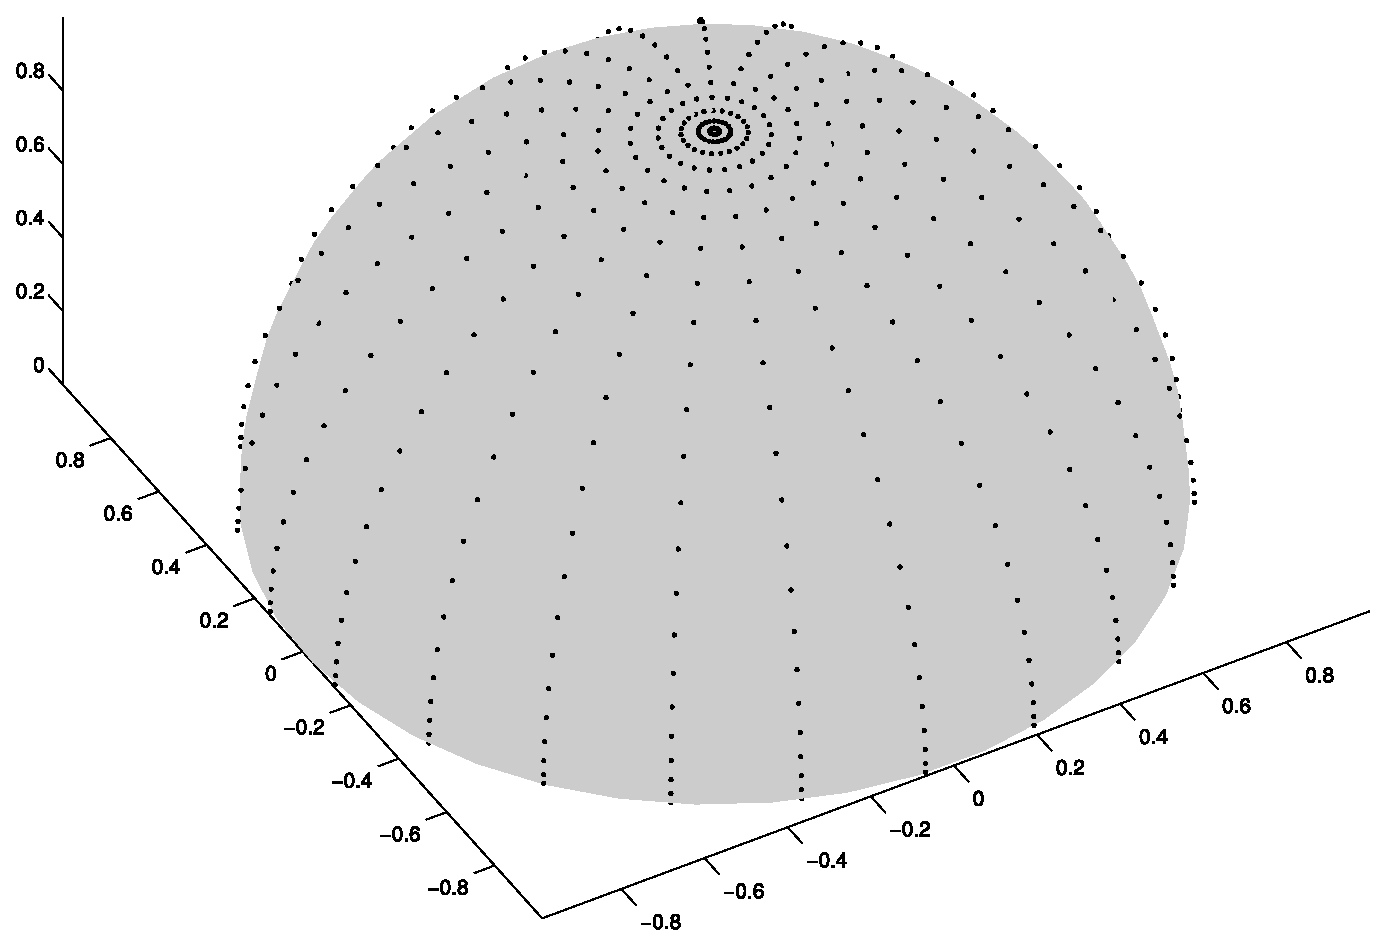
\includegraphics[height=.4\textheight]{quad22mod.eps}
\caption{Расположение узлов квадратуры для полусферы для случая $n = 22$}
\label{fig:quad22}
\end{figure}

\paragraph{Сведение к квадратуре гауссового типа.} Для интеграла
\[
I = \int\limits_0^{\pi/2} S(\cos \theta, \sin \theta) \cos \theta \sin \theta d\theta
\]
сделаем замену переменной $\theta = \frac{\pi}{4} + 2 \arctg \xi$. При этом
\begin{gather*}
r = \cos \theta = \cos \left(\frac{\pi}{4} + 2 \arctg \xi\right) = \frac{1 - 2 \xi - \xi^2}{\sqrt{2}(1 + \xi^2)},\\
z = \sin \theta = \sin \left(\frac{\pi}{4} + 2 \arctg \xi\right) = \frac{1 + 2 \xi - \xi^2}{\sqrt{2}(1 + \xi^2)},\\
Q(r, z) = \frac{W_{2n}(\xi)}{(1 + \xi^2)^n},\qquad d\theta = \frac{2d\xi}{1 + \xi^2},
\end{gather*}
где $W_{2n}(\xi)$ --- многочлен степени не выше $2n$, а сам интеграл принимает вид
\[
I = \int\limits_{1-\sqrt{2}}^{\sqrt{2} - 1}
W_{2n}(\xi) \frac{(1 - \xi^2)^2 - 4\xi^2}{(1 + \xi^2)^{n+3}} d\xi.
\]
Если рассматривать $\omega(\xi) = \frac{(1 - \xi^2)^2 - 4\xi^2}{(1 + \xi^2)^{n+3}} $ в качестве веса, получается классическая задача для построения Гауссовой квадратурной формулы с весом. Для этой задачи разработаны устойчивые вычислительные алгоритмы, например, алгоритм Голуба-Велша \cite{Golub1969}.
Для точного интегрирования многочленов степени $2n$ необходимо и достаточно использовать $n+1$ узел гауссовой квадратуры.
При этом, в силу симметрии весовой функции $\omega(\xi) = \omega(-\xi)$, полученные узлы будут симметричны относительно $\xi = 0$, что гарантирует симметрию $\theta_j = \frac{\pi}{2} - \theta_{n - j}$ для узлов исходной квадратурной формулы.

Хотя задача построения квадратурной формулы для полусферы и может быть сведена к построению гауссовой квадратуры, метод продолжения по параметру был успешно применен для построения и других квадратурных формул, для которых данное сведение не известно.


\section{Решение линейной системы}

Для решения линейной системы \eqref{eq:operator2} применялся метод сопряженных градиентов. Это было обусловлено несколькими факторами:
\begin{itemize}
\item во-первых, так как матрица  $\mathcal A$ системы является положительно определенной и симметричной, метод гарантированно сходится (без учета ошибок округления);
\item во-вторых, для работы метода не требуется знания границ спектра матрицы  $\mathcal A$;
\item в-третьих, метод работает не с матрицей $\mathcal A$ напрямую, а лишь с матрично-векторным произведением  $\mathcal{A} \varphi$;
\item в-четвертых, метод позволяет использовать предобуславливатель для системы.
\end{itemize}

Как было отмечено выше, решение линейной системы соответствует решению дискретизированной системы эллиптических уравнений. Известно \cite{samarskiy1977,fedorenko1994}, что эллиптические операторы являются энергетически эквивалентными. Это свойство имеется и у их дискретных аналогов. Если в качестве предобуславливателя для данной задачи взять дискретный аналог некоторой другой системы эллиптических уравнений, то число обусловленности предобусловленной системы, а с ним и количество итераций метода, должно слабо зависеть от подробности пространственной сетки.

Матрица системы может быть представлена в блочном виде, где каждый блок содержит пространственную дискретизацию некоторого скалярного эллиптического оператора. Пользуясь кронекеровским произведением, объемная часть матрицы $\mathcal{A}$ может быть записана как
\[
\mathcal{A}^\text{объёмн} = \mathscr{H} \otimes M + \sum_{\alpha,\beta} \mathscr{K}^{\alpha\beta} \otimes S_{\alpha\beta}.
\]
Если из матриц $\mathscr{H}, \mathscr{K}^{\alpha\beta}$ удалить внедиагональные элементы, то полученная матрица
\begin{equation}
\mathcal{M}^\text{объёмн} = \operatorname{diag}(\mathscr{H}) \otimes M + \sum_{\alpha,\beta}  \operatorname{diag}(\mathscr{K})^{\alpha\beta} \otimes S_{\alpha,\beta}
\label{eq:precondop}
\end{equation}
будет соответствовать некоторой другой системе эллиптических уравнений, энергетически эквивалентной исходной. Заметим, что из-за блочно-диагональной структуры $\mathcal{M}$, она фактически соответствует набору из независимых скалярных эллиптических уравнений. Напротив, матрица $\mathcal{A}$ соответствовала связанной системе эллиптических уравнений.
Обозначим $\mathcal{A}^{(k,k')}$ блок матрицы $\mathcal{A}$ с координатами $(k, k')$. Тогда
\[
\mathcal{M}^{(k,k')} = \begin{cases}
\mathcal{A}^{(k,k)}, & k = k'\\
0, &k \neq k'.
\end{cases}
\]

Другая интерпретация процесса удаления внедиагональных блоков из матрицы $\mathcal{A}$ может быть дана в терминах минимизации функционала $\mathcal{G}$. Если решение системы с матрицей $\mathcal{A}$ эквивалентно решению задачи минимизации \eqref{eq:minimize}
\[
\mathcal{G}(\varphi(\vec r, \vec \Omega)) \to \min_{\varphi(\vec r, \vec \Omega) \in \mathcal{H}_0}
\]
одновременно по всем угловым гармоникам решения $\varphi_k(\vec r)$, то решение системы с матрицей $\mathcal{M}$ соответствует решению задач минимизации
\[
\mathcal{G}(\varphi_{k}(\vec r) \theta_k(\vec \Omega)) \to \min_{\varphi_k(\vec r)}, \quad k = 1, \dots, K.
\]
отдельно для каждой гармоники $\varphi_k(\vec r)$. 

Стандартный предобусловленный вариант метода сопряженных градиентов приведен в алгоритме \ref{alg:precondcgs}, где в качестве предобуславливателя используется блочная диагональ матрицы $\mathcal {A}$.

\begin{algorithm}[ht!]
\centering
\begin{algorithmic}[1]
\Function{ConjugateGradients}{$\mathcal{A}$, $f$, $\varphi$, $tol = 10^{-6}$}
\State $r = f - $ \Call{Product}{$\mathcal{A}$, $\varphi$}
\State $resinit := ||r||^2$
\For {$i = 1, \dots, K$} 
\State $z_i := $ \Call{PreconditionerSolve}{$\mathcal{A}^{(i,i)}$, $r_i$}
\EndFor
\State $p = z$
\State $rz = (r, z)$
\Repeat
\State $Ap := $ \Call{Product}{$\mathcal{A}$, $p$}
\State $pAp := (p, Ap)$
\State $\alpha := {rz}/{pAp}$
\State $\varphi := \varphi + \alpha p$
\State $r := r - \alpha Ap$
\If {$||r||^2 < resinit \cdot tol^2$}
\State \Return $\varphi$
\EndIf
\For {$i = 1, \dots, K$} 
\State $z_i := $ \Call{PreconditionerSolve}{$\mathcal{A}^{(i,i)}$, $r_i$}
\EndFor
\State $rznew := (r, z)$
\State $\beta := {rznew}/{rz}$
\State $rz := rznew$
\State $p := z + \beta p$
\Until \textbf{false}
\EndFunction
\end{algorithmic}
\caption{Предобусловленный метод сопряженных градиентов}
\label{alg:precondcgs}
\end{algorithm}

В функции \textsc{PreconditionerSolve} также использовался метод сопряженных градиентов, но без предобуславливания. Для этой задачи подойдет любой метод, предназначенный для решения систем линейных уравнений, полученных в результате дискретизации эллиптических операторов вида
\[
-\div \frac{1}{\varkappa} \mathbb D \grad \phi + \varkappa \varphi.
\]
В данной работе изучалась сходимость именно внешних итераций, без учета сходимости самого процесса предобуславливания. 

\section{Вычисление физических характеристик излучения}

Достаточно часто для практических приложений необходима не сама функция интенсивности излучения $I(\vec x, \vec \Omega)$, а лишь ее интегральные характеристики --- плотность и поток энергии, тензор потока импульса и т. п. Рассмотрим обобщенный четный момент функции интенсивности
\[
J_{\alpha\beta\dots\lambda}(\vec r) \equiv \int\limits_{4\pi} \Omega_\alpha \Omega_\beta \cdots \Omega_\lambda I(\vec r, \vec \Omega) d\Omega.
\]
В силу четности интеграла относительно замены $\vec \Omega \to -\vec \Omega$, подынтегральную функцию интенсивности можно заменить на ее четную часть $\varphi(\vec r, \vec \Omega)$:
\[
J_{\alpha\beta\dots\lambda}(\vec r) = \int\limits_{4\pi} \Omega_\alpha \Omega_\beta \cdots \Omega_\lambda \varphi(\vec r, \vec \Omega) d\Omega.
\]
Принимая во внимание разложение по угловым базисным функциям
\[
\varphi(\vec r, \vec \Omega) = \sum_{k = 1}^{K} \varphi_k(\vec r) \theta_k(\vec \Omega),
\]
получаем
\[
J_{\alpha\beta\dots\lambda}(\vec r) = \sum_{k=1}^{K} \Theta_k^{\alpha\beta\dots\lambda} \varphi_k(\vec r),
\]
где угловые моменты базисных функций $\Theta_k^{\alpha\beta\dots\lambda}$ определяются как
\[
\Theta_k^{\alpha\beta\dots\lambda} \equiv \int\limits_{4\pi} \Omega_\alpha \Omega_\beta \cdots \Omega_\lambda \theta_k(\vec \Omega) d\Omega.
\]
Например, 
\begin{gather*}
U(\vec r) \equiv \frac{1}{c}\int\limits_{4\pi} I(\vec r, \vec \Omega) d\Omega = \frac{1}{c} J(\vec r) = \frac{1}{c} \sum_{k=1}^{K} \Theta_k \varphi_k(\vec r)\\
\mathbb T_{\alpha\beta}(\vec r) \equiv \frac{1}{c}\int\limits_{4\pi} \Omega_\alpha \Omega_\beta I(\vec r, \vec \Omega) d\Omega = \frac{1}{c} J_{\alpha\beta}(\vec r) = \frac{1}{c} \sum_{k=1}^{K} \Theta_k^{\alpha\beta} \varphi_k(\vec r).
\end{gather*}
Для базиса из радиальных функций $\theta_k(\vec \Omega) = R_k(\vec \Omega)$ значения $\theta_{k}^{\cdot}$ могут быть найдены численным интегрированием с помощью квадратурной формулы Лебедева, а для базиса из сферических функций $\theta_k(\vec \Omega) = Y_{l,m}(\vec \Omega)$ эти выражения можно найти аналитически.

Для плотности энергии излучения используются нулевые моменты базисных функций
\[
\Theta_k = \int\limits_{4\pi} \theta_k(\vec \Omega) d\Omega = 
\int\limits_{4\pi} Y_{l,m}(\vec \Omega) d\Omega = 
\begin{cases}
4\pi, &l = 0\\
0, &l \neq 0.
\end{cases}
\]
Таким образом, для метода сферических гармоник
\[
U(\vec r) = \frac{4\pi}{c} \varphi_{0,0}(\vec r).
\]

Для тензора потока импульса излучения используются вторые моменты базисных функций
\[
\Theta_k^{\alpha\beta} = \int\limits_{4\pi} \Omega_{\alpha}\Omega_{\beta}\theta_k(\vec \Omega) d\Omega 
= \int\limits_{4\pi} \Omega_{\alpha}\Omega_{\beta} Y_{l,m}(\vec \Omega) d\Omega.
\]
Заметим, что тензор $\Omega_\alpha\Omega_\beta$ является однородным многочленом второй степени относительно $\vec \Omega$, а, следовательно, раскладывается в линейную комбинацию функций $Y_{l,m}(\vec \Omega)$. 
\begin{multline}
%\begin{pmatrix}
%\Omega_x^2 & \Omega_x \Omega_y & \Omega_x \Omega_z\\
%\Omega_x \Omega_y & \Omega_y^2 & \Omega_y \Omega_z\\
%\Omega_x \Omega_z & \Omega_y \Omega_z & \Omega_z^2
%\end{pmatrix} = \\ =
\Omega_\alpha\Omega_\beta = 
\begin{pmatrix}
\frac{1}{3}Y_{0,0} - \frac{\sqrt{5}}{15} Y_{2,0} + \frac{1}{\sqrt{15}}Y_{2,2}& \frac{1}{\sqrt{15}}Y_{2,-2} & \frac{1}{\sqrt{15}}Y_{2,1} \\
\frac{1}{\sqrt{15}}Y_{2,-2} &\frac{1}{3}Y_{0,0} - \frac{\sqrt{5}}{15} Y_{2,0} - \frac{1}{\sqrt{15}}Y_{2,2} & \frac{1}{\sqrt{15}}Y_{2,-1}\\
\frac{1}{\sqrt{15}}Y_{2,1} & \frac{1}{\sqrt{15}}Y_{2,-1} & \frac{2\sqrt{5}}{15}Y_{2,0} + \frac{1}{3}Y_{0,0}
\end{pmatrix}
\label{eq:oaob}
\end{multline}
Пользуясь ортогональностью функций $Y_{l,m}$, получаем
\begin{alignat*}{5}
&\Theta^{\alpha\beta}_{0,0} &= \frac{4\pi}{3}\begin{pmatrix}
1 & 0 & 0\\
0 & 1 & 0\\
0 & 0 & 1
\end{pmatrix}\qquad
&\Theta^{\alpha\beta}_{2,-2} &&= \frac{4\pi}{\sqrt{15}}\begin{pmatrix}
0 & 1 & 0\\
1 & 0 & 0\\
0 & 0 & 0
\end{pmatrix}\\
&\Theta^{\alpha\beta}_{2,-1} &= \frac{4\pi}{\sqrt{15}}\begin{pmatrix}
0 & 0 & 0\\
0 & 0 & 1\\
0 & 1 & 0
\end{pmatrix}\qquad
&\Theta^{\alpha\beta}_{2,0} &&= \frac{4\pi\sqrt{5}}{15}\begin{pmatrix}
-1 & 0 & 0\\
0 & -1 & 0\\
0 & 0 & 2
\end{pmatrix}\\
&\Theta^{\alpha\beta}_{2,1} &= \frac{4\pi}{\sqrt{15}}\begin{pmatrix}
0 & 0 & 1\\
0 & 0 & 0\\
1 & 0 & 0
\end{pmatrix}\qquad
&\Theta^{\alpha\beta}_{2,2} &&= \frac{4\pi}{\sqrt{15}}\begin{pmatrix}
1 & 0 & 0\\
0 & -1 & 0\\
0 & 0 & 0
\end{pmatrix}.
\end{alignat*}
Остальные $\Theta^{\alpha\beta}_{l,m}$ равны нулю, таким образом
\[
\mathbb T_{\alpha\beta}(\vec r) = \frac{1}{c}\left[
\Theta^{\alpha\beta}_{0,0} \varphi_{0,0}(\vec r) + 
\sum_{m=-2}^{2} \Theta^{\alpha\beta}_{2,m} \varphi_{2,m}(\vec r)
\right].
\]

Для нахождения нечетных моментов интенсивности, например, потока энергии излучения $\vec S$
\[
\vec S \equiv \int\limits_{4\pi} \vec \Omega I(\vec r, \vec \Omega) d\Omega
\]
необходимо привлекать дифференциальное уравнение переноса \eqref{eq:transf2}.
\[
\frac{1}{\varkappa(\vec r)} \Omega_\alpha \nabla_\alpha I(\vec r, \vec \Omega) + I(\vec r, \vec \Omega) = I_\text{p}(\vec r, \vec \Omega).
\]
Интегрируя его с весом $\Omega_\beta\dots\Omega_\lambda$, получаем
\[
\frac{1}{\varkappa(\vec r)} \nabla_\alpha J_{\alpha\beta\dots\lambda}(\vec r) + 
J_{\beta\dots\lambda}(\vec r) = 0.
\]
В последней формуле учтено, что $I_\text{p}$ --- четная по $\vec \Omega$ функция и ее нечетные моменты равны нулю. Таким образом, справедливо соотношение
\[
J_{\beta\dots\lambda}(\vec r) = -\frac{1}{\varkappa(\vec r)} \nabla_\alpha J_{\alpha\beta\dots\lambda}(\vec r),
\]
которое связывает нечетные моменты функции интенсивности с пространственными производными от четных моментов. Например, для $\vec S$ верно
\[
[\vec S]_\alpha(\vec r) = J_\alpha(\vec r) = -\frac{1}{\varkappa(\vec r)} \nabla_\beta J_{\alpha \beta}(\vec r) = -\frac{c}{\varkappa(\vec r)} \nabla_\beta \mathbb T_{\alpha\beta}(\vec r).
\]

\section{Реализация метода с использованием графических ускорителей}

Самый трудоемкий этап при решении системы линейных алгебраических уравнений методом сопряженных градиентов --- это непосредственно
этап вычисления по заданному вектору $\varphi$ результата действия на него оператора задачи
$[\mathcal{A}\varphi]_{i,k} = [\phi_i(\vec r)\theta_k(\vec \Omega), \varphi(\vec r, \vec \Omega)]$, см. \cite{miptconf53}. Оператор задачи можно разбить на 
объемную и поверхностную части
\begin{align*}
[\mathcal{A}^\text{объемн} \varphi]_{i,k} &= \left(\phi_i\theta_k, \varphi\right) + 
\left(\frac{1}{\varkappa}(\vec \Omega \nabla)\phi_i\theta_k, \frac{1}{\varkappa}(\vec \Omega \nabla)\varphi\right)\\
[\mathcal{A}^\text{поверх} \varphi]_{i,k} &= \iint\limits_{\partial G \times 4\pi} \phi_i\theta_k \varphi d\Gamma d\Omega.
\end{align*}
В обозначениях \eqref{eq:operator2}
\begin{align*}\nonumber
[\mathcal{A}^\text{объемн} \varphi]_{i,k}  &= \sum_{k'} \mathscr{H}_{kk'}\sum_{T_j \ni \vec r_i}\int\limits_{T_j} \varkappa \phi_i \varphi_{k'} d\vec r +\\
&+\sum_{k',\alpha,\beta} \mathscr{K}_{kk'}^{\alpha\beta}
\sum_{T_j \ni \vec r_i}\int\limits_{T_j} \frac{1}{\varkappa} (\nabla_\alpha\phi_i)(\nabla_\beta\varphi_{k'}) d\vec r\\
[\mathcal{A}^\text{поверх} \varphi]_{i,k} &= \sum_{T_j \ni \vec r_i}
\sum_{k'}\mathscr{B}_{kk'}(\vec n)
\int\limits_{\partial T_j \cap \partial G} 
\phi_i \varphi_{k'} d\Gamma.
\end{align*}

В программной реализации сначала параллельно по гармоникам решения вычисляются пространственные интегралы.
Это производится с помощью построенных в параграфе \ref{sec:quad} квадратурных формул. Квадратурные формулы удобны тем, что для вычисления интегралов достаточно знать лишь значения функции $\varphi_{k'}(\vec r)$ в вершинах тетраэдра и номер вершины тетраэдра, которому соответствует точка $\vec r_i$.
Затем, полученные вектора значений умножается на матрицы $\mathscr{H}_{kk'}, \mathscr{K}_{kk'}^{\alpha\beta}, \mathscr{B}_{kk'}$.
Последняя операция --- коллективная, и требует обмена данными между потоками. Более того, в архитектуре CUDA обмен данными 
между потоками возможен только через специальную разделяемую память. Оценим объем необходимой разделяемой памяти для 
вычисления решения в конкретной точке. В разделяемой памяти должно размещаться $3 \times 3 \times K$ величин типа 
\textsf{double}. Учитывая ограничение в $\sim 48$ КБайт разделяемой памяти на каждый параллельный блок в архитектуре CUDA,
получаем, что один такой блок может обрабатывать не более $K \sim 600$ направлений. При этом параллельный блок будет обрабатывать одну вершину $\vec r_i$. 
Аппаратно это означает, что для вычисления всех гармоник $[\mathcal{A}^\text{объемн} \varphi]_{i,k}$ в точке $\vec r_i$ будет задействован целый мультипроцессор.
Это довольно расточительно с точки зрения ресурсов, но необходимость во взаимодействии потоков с разными значениями $k'$ неизбежна.
Заметим, что взаимодействие между разными гармониками решения отсутствует при вычислениях с диагональным эллиптическим оператором \eqref{eq:precondop}, что позволяет существенно быстрее решать задачу методом сопряженных градиентов для предобуславливателя.

Вычисление пространственных частей оператора тоже создает некоторые трудности. В каждой точке необходимо вычислять сумму выражений
по всем тетраэдрам или треугольникам, содержащим данную точку. Значит, номера этих тетраэдров и треугольников должны быть заранее 
найдены и переданы в процедуру вычисления действия оператора $\mathcal A$ на вектор $\varphi$. Можно оценить объём памяти, занимаемый описанием пространственной 
сетки вместе с этой вспомогательной информацией.

Допустим, что сетка содержит $N$ точек. В каждой точке сходится порядка $20$ 
тетраэдров\footnote{Телесный угол при вершине правильного тетраэдра равен $\arccos \frac{23}{27} \approx 0.551\text{ ср} \approx \frac{4\pi\text{ ср}}{23}$. }.
Значит количество тетраэдров $N_t$ порядка $\frac{20N}{4} = 5N$. Это число хорошо согласуется с реальными сетками.

В программе расчетная сетка хранится в следующей форме
\begin{itemize}
	\item $N_t \approx 5N$ структур размера $128$ байт, описывающих тетраэдры со следующими полями
	\begin{itemize}
	\item $4$ числа типа \textsf{unsigned int} --- номера вершин тетраэдра
	\item $1$ число типа \textsf{double} --- произведение $\varkappa V$
	\item $1$ число типа \textsf{double} --- равновесная интенсивность $I_\text{p}$
	\item $12$ чисел типа \textsf{double} --- векторные площади четырех граней $\vec S^j_\alpha$
	\end{itemize}
	\item $\sim 20N$ пар чисел типа \textsf{unsigned int} --- номера тетраэдров, содержащих точку $\vec r_i$ и локальный номер вершины, совпадающей с $\vec r_i$
\end{itemize}

Размером аналогичных структур, описывающих граничные треугольники, пренебрежем. Суммарно расчетная сетка занимает порядка $800N$ байт.
Заметим, что при этом вектор решения системы линейных уравнений занимает $8 K N$ байт, и для случая $K = 50$ это уже
$400N$ байт. Учтем, что для реализации метода сопряженных градиентов необходимо четыре вектора такого размера, а для реализации
метода сопряженных градиентов с предобуславливанием --- пять (для самого метода) и еще три (для самого предобуславливателя).
Получается, что необходимый объем памяти определяется не сложной структурой расчетной сетки, а многомерностью вектора неизвестных и вспомогательных векторов.

Для метода сферических гармоник матрица $\mathscr{H}_{kk'}^{\alpha\beta}$ является разреженной. Рассмотрим блок $3\times 3$ данной матрицы, имеющий координаты $(k,k')$:
\[
\mathscr{H}_{kk'}^{\alpha\beta} \equiv \int\limits_{4\pi} \Omega_\alpha\Omega_\beta \theta_{k}(\vec \Omega) \theta_{k'}(\vec \Omega) d\Omega.
\]
Ранее было показано, что $ \Omega_\alpha\Omega_\beta$ выражается через линейную комбинацию $Y_{0,0}, Y_{2,m}$, а, значит, $\mathscr{H}_{kk'}^{\alpha\beta}$ --- линейная комбинация интегралов от трех сферических функций:
\[
\mathscr{H}_{l,m,l',m'}^{\alpha\beta} = 
\int\limits_{4\pi} \Omega_\alpha\Omega_\beta Y_{l,m}(\vec \Omega) Y_{l',m'}(\vec \Omega) d\Omega = 
\sum_{\lambda = 0,2}\sum_{\mu = -\lambda}^{\lambda} c_{\alpha\beta}^{\lambda\mu} \begin{bmatrix}
\lambda & l & l'\\
\mu & m & m'
\end{bmatrix}.
\]
Символ $\begin{bmatrix}
\lambda & l & l'\\
\mu & m & m'
\end{bmatrix}$ определяется как
\[
\begin{bmatrix}
\lambda & l & l'\\
\mu & m & m'
\end{bmatrix} = \int\limits_{4\pi} 
Y_{\lambda,\mu}(\vec \Omega)
Y_{l,m}(\vec \Omega)
Y_{l',m'}(\vec \Omega) d\Omega.
\]
Данный интеграл не обращается в ноль только если выполнены правила отбора, приведенные в параграфе \ref{sec:select}. В частности, при $|l - l'| > 2$ интеграл равен нулю, поскольку $\lambda, l, l'$ не удовлетворяют неравенству треугольника.

Рассмотрим возможные значения для $\mu$ в элементах матрицы $\Omega_\alpha\Omega_\beta$, см. \eqref{eq:oaob}:
\[
\mu(\Omega_\alpha\Omega_\beta) = \begin{pmatrix}
0,2& -2 & 1\\
-2 & 0,2 & -1\\
1 & -1 & 0
\end{pmatrix}
\]

Рассмотрим различные возможные значения $m, m'$. Пусть для определенности $m \leq m'$. Если $m = 0$, то в матрице $\mathscr{K}_{l,m,l',m'}^{\alpha\beta}$ остаются ненулевыми только элементы с 
$m' \in \mu(\Omega_\alpha\Omega_\beta)$, причем для любого значения $m'$ в матрице остается не более одного ненулевого элемента. Аналогично для $m' = 0$.

Заметим, что во всех случаях четность суммы $m + m' + \mu$ является необходимым условием нетривиальности интеграла.

Если $m, m' < 0$, то в матрице $\mathscr{K}_{l,m,l',m'}^{\alpha\beta}$ ненулевыми будут лишь элементы с положительными $\mu(\Omega_\alpha\Omega_\beta)$. Так как в строках нет положительных элементов одинаковой четности, снова в каждой строке не более одного ненулевого элемента.

Если $m < 0 < m'$, то в матрице $\mathscr{K}_{l,m,l',m'}^{\alpha\beta}$ ненулевыми будут лишь элементы с отрицательными $\mu(\Omega_\alpha\Omega_\beta)$. Так как в строках нет отрицательных элементов одинаковой четности, снова в каждой строке не более одного ненулевого элемента.

В последнем случае $0 < m < m'$, в матрице $\mathscr{K}_{l,m,l',m'}^{\alpha\beta}$ ненулевыми будут лишь элементы c положительными $\mu(\Omega_\alpha\Omega_\beta)$. Случай аналогичен $m, m' > 0$.

Таким образом, для всех возможных значений $m, m'$ матрицы $\mathscr{K}_{l,m,l',m'}^{\alpha\beta}$ содержат не более одного ненулевого элемента в каждой строке блока $3 \times 3$, что позволяет уменьшить необходимый объем хранимых данных. Вид данной матрицы при $K = 6$ приведен в параграфе \ref{sec:oioj}           % Глава 2
\chapter{Маршевый метод коротких характеристик}

\section{Численные методы для стационарных гиперболических задач}

Уравнение переноса излучения относится к классу стационарных гиперболических уравнений. Стационарное гиперболическое уравнение должно содержать времениподобную переменную. Например, для задачи сверхзвукового обтекания такой переменной может быть выбрано направление, в котором поток газа или жидкости движется со сверхзвуковой скоростью. Для задачи переноса излучения времениподобной переменной является координата $s$ вдоль направления излучения $\vec \Omega$. 

Для гиперболических уравнений разработан ряд методов, например, сеточно-характеристические методы \cite{magometov1988}, различные TVD методы \cite{Godunov1959,vanLeer1974,Leveque2002,Toro2009}, ENO и WENO схемы \cite{Shu1998} и разрывный метод Галеркина \cite{Cockburn1989}. Для применения этих методов к уравнению переноса следует сначала дискретизировать угловую часть функции интенсивности $I(\vec r, \vec \Omega) \to I_i(\vec r)$. Для этой задачи имеется два основных подхода:
\begin{itemize}
\item дискретизация на некоторой сетке направлений $\vec \omega_i$, при этом $I_i(\vec r) = I(\vec r, \vec \omega_i)$;
\item дискретизация усреднением.
\end{itemize}
В последнем случае сфера направлений разбивается на участки $\Sigma_i$, например, триангулируется. Далее, уравнение переноса 
\[
(\vec \Omega \nabla) I(\vec r, \vec \Omega) + \varkappa(\vec r, \vec \Omega) I(\vec r, \vec \Omega) = \varkappa(\vec r, \vec \Omega) I_\text{p}(\vec r, \vec \Omega),
\]
которое можно записать в дивергентном виде
\[
\div \left(\vec \Omega I(\vec r, \vec \Omega)\right) + \varkappa(\vec r, \vec \Omega) I(\vec r, \vec \Omega) = \varkappa(\vec r, \vec \Omega) I_\text{p}(\vec r, \vec \Omega),
\]
усредняется по каждому участку $\vec \Omega \in \Sigma_i$. При этом
\[
I_i(\vec r) = \int\limits_{\Sigma_i} I(\vec r, \vec \Omega) d\Omega,
\]
а при усреднении $\vec \Omega I(\vec r, \vec \Omega)$ обычно предполагается зависимость среднего только от $I_i(\vec r)$:
\[
\int\limits_{\Sigma_i} \vec \Omega I(\vec r, \vec \Omega) d\Omega \sim I_i(\vec r).
\]
Если обозначить
\[
\vec \omega_i \equiv \frac{\int_{\Sigma_i} \vec \Omega I(\vec r, \vec \Omega) d\Omega}{\int_{\Sigma_i} I(\vec r, \vec \Omega) d\Omega},
\]
усредненное уравнение переноса принимает простой вид, аналогичный уравнению, дискретизированному на сетке направлений $\vec \omega_i$
\begin{equation}
\div (\vec \omega_i I_i(\vec r)) + \varkappa_i(\vec r) I_i(\vec r) = \varkappa_i(\vec r) I_{\text{p},i}(\vec r),\quad i = 1, \dots, K.
\label{eq:grid}
\end{equation}

Вне зависимости от способа получения, система \eqref{eq:grid} является системой независимых уравнений переноса в направлениях $\vec \omega_i$, и может быть решена вдоль всех направлений параллельно. Необходимо отметить, что метод, построенный на основании системы \eqref{eq:grid}, всегда будет испытывать <<эффект луча>>, так как излучение от источника может распространяться только в направлениях $\vec \omega_i$ и ни в каких других.



Рассмотрим отдельно $i$-е уравнение. Характеристикой данного уравнения является луч $\vec r - \vec r_0 = \vec \omega_i s$. 
Для уравнения переноса сеточно-характеристический метод называется методом коротких характеристик В метода коротких характеристик лежит идея интерполяции сеточных величин в основании характеристики $I_i^*$ и дальнейшего интегрирования решения уравнения вдоль характеристики (см. рисунок \ref{fig:char}). При этом найти решение в точке $\vec r_p$, из которой выпущена характеристика возможно лишь после того, как во всех узлах грани, содержащей основание характеристики, решение уже найдено. Будем далее назвать грань \emph{освещенной}, если интенсивность излучения $I_i$ во всех узлах на ней известна.
\begin{figure}[ht!]
\centering
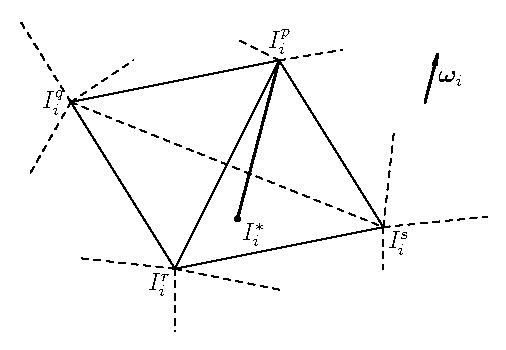
\includegraphics[height=.3\textheight]{radiation-2.eps}
\caption{Схема сеточно-характеристического метода}
\label{fig:char}
\end{figure}

Простейшим представителем конечно-объёмных методов является метод Годунова. В основе конечно-объемных методов лежат интегральные законы сохранения. Проинтегрируем уравнение переноса
\eqref{eq:grid} по объему тетраэдра $T$ (для краткости будем опускать индекс направления $i$):
\[
\int\limits_T \div (\vec \omega I(\vec r))  d\vec r + \int\limits_T \varkappa(\vec r) I(\vec r)  d\vec r = \int\limits_T \varkappa(\vec r) I_\text{p}(\vec r)  d\vec r.
\]
Интеграл от дивергенции может быть записан в виде интеграла по границе:
\[
\int\limits_T \div (\vec \omega I(\vec r)) d\vec r= \int_{\partial T} \vec n \vec \omega I(\vec r) d\Gamma.
\]
В конечно-объемных методах нормальный поток на границе конечного объема определяется из точного либо приближенного решения задачи Римана о распаде разрыва \cite{Kulikovskiy2001}.
Для уравнения переноса излучения задача Римана имеет простое решение. Пусть значение интенсивности излучения в полупространстве $\vec r \vec n < 0$ равно $I_L$, а значение в полупространстве $\vec r \vec n > 0$ равно $I_R$. Тогда поток интенсивности излучения $\vec \omega I$ через границу $\vec r \vec n = 0$ равен
\[
\vec \omega I\big|_{\vec r \vec n = 0} = 
\begin{cases}
\vec \omega I_L, &\vec \omega \vec n > 0\\
\vec \omega I_R, &\vec \omega \vec n \leq 0
\end{cases}.
\] 
Заметим, что отнесение $\vec \omega \vec n = 0$ к одному из этих случаев несущественно, так как нормальный поток в любом случае будет равен нулю.

Назовем грань $f_j$ тетраэдра $T$ \emph{входной}, если внешняя нормаль $\vec n_j$ составляет с направлением изучения $\vec \omega$ тупой угол, и \emph{выходной} в противном случае.
Примем гипотезу о постоянном распределении величин $I, \varkappa, I_{\text{p}}$ в тетраэдре $T$. Обозначим $I^0$ интенсивность излучения в тетраэдре $T$, а $I^j$ --- интенсивность излучения в тетраэдре, граничащем с $T$ по грани $f_j$. Используя выражение для нормального потока из решения задачи Римана, получаем метод Годунова для уравнения переноса излучения:
\begin{equation}
\frac{1}{V(T)}\left[
\sum_{\substack{f_j \in \partial T\\\vec n_j \vec \omega < 0}} \vec S_j \vec \omega I^j 
+
\sum_{\substack{f_j \in \partial T\\\vec n_j \vec \omega > 0}} \vec S_j \vec \omega I^0
\right]
+ \varkappa I^0 = \varkappa I_\text{p},
\label{eq:fvm}
\end{equation}
где посредством $\vec S_j$обозначена векторная площадь грани $j$, то есть площадь, умноженная на внешнюю нормаль $\vec n_j$, а $V(T)$ --- объём тетраэдра $T$. Можно видеть, что для определения $I^0$ необходимо знать интенсивность излучения $I^j$ во всех тетраэдрах, граничащих с $T$ по его входным граням.

Разностные задачи, полученные либо сеточно-характеристичекими, либо конечно-объёмными методами, представляют собой набор линейных уравнений относительно неизвестных значений интенсивности. Данные уравнения можно решить итерационно, например методом установления, фактически превратив исходную стационарную гиперболическую задачу в нестационарную. Однако, эти задачи могут быть решены и безытерационным методами, в которых решение строится последовательным обходом неизвестных (маршем), при котором для вычисления очередной неизвестной все необходимые данные были найдены раньше.
Данные методы имеют преимущество, так как требуют лишь однократного прохода по расчетной области, в отличие от итерационных методов, в которых необходимо многократно повторять вычисления для каждого узла до достижения требуемой точности.

\section{Метод коротких характеристик второго порядка аппроксимации}

Рассмотрим метод коротких характеристик, в котором интенсивность излучения задана в нескольких узлах на гранях тетраэдров, но без конкретизации расположения данных узлов и их количества. Будем предполагать, что коэффициенты поглощения и интенсивность равновесного излучения постоянны в каждом тетраэдре.

Для определения решения на грани требуется определить решение в каждом узле, расположенном на данной грани. Для этого из каждого узла грани выпускается характеристика в направлении $-\vec\omega$ до пересечения с гранью тетраэдра (см. рисунок \ref{fig:manychar}). Заметим, что эта грань будет входной, так как характеристика выходит из тетраэдра в направлении $-\vec\omega$ под острым углом к нормали $\vec n$ к грани. Различные характеристики могут выходить из тетраэдра через различные входные грани, поэтому до вычисления решения на выходной грани, все входные грани должны быть уже освещены (то есть, решение на них уже должно быть найдено).
\begin{figure}[ht!]
\centering
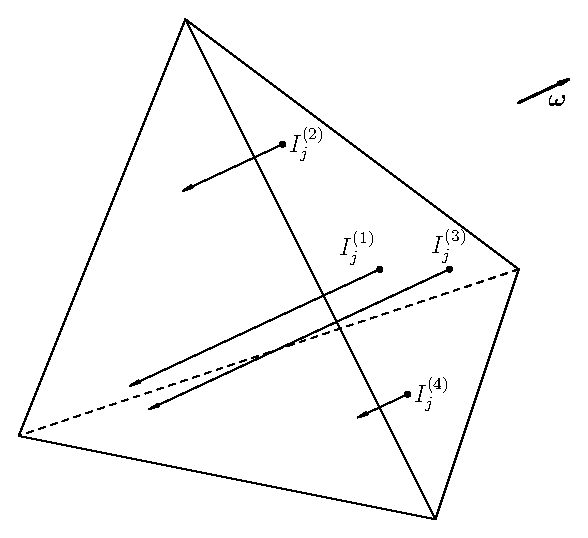
\includegraphics[height=.3\textheight]{radiation-4.eps}
\caption{Характеристики, выпущенные из нескольких узлов на грани тетраэдра}
\label{fig:manychar}
\end{figure}

Вдоль каждой характеристики уравнение переноса является обыкновенным дифференциальным уравнением
\[
\frac{dI}{ds} + \varkappa I = \varkappa I_\text{p},
\]
причем величины $\varkappa$ и $I_\text{p}$ постоянны по предположению. Решение этого уравнения может быть записано в виде
\begin{equation}
I = e^{-\tau} I^*  + \left(1 - e^{-\tau}\right) I_\text{p},
\label{eq:shortchar}
\end{equation}
где $I$ --- интенсивность излучения в точке, из которой выпускается характеристика, $I^*$ --- интенсивность излучения в точке пересечения характеристики с входной гранью, а $\tau$ --- оптическая длина характеристики, равная ее длине $\ell$, умноженной на коэффициент поглощения $\varkappa$. Из \eqref{eq:shortchar} следует, что интенсивность $I$ не выходит за диапазон значений $[\min(I^*, I_\text{p}), \max(I^*, I_\text{p})]$.

Величина $I^*$ определяется интерполяцией по значениям интенсивности в узлах той грани, через которую выходит характеристика. Порядок аппроксимации метода соответствует степени используемой интерполяции. Для получения метода второго порядка необходимо пользоваться квадратичной интерполяцией значений интенсивности на грани, при этом необходимо знать значение интенсивности в шести узлах на данной грани.

Повысить порядок метода можно и не увеличивая количество узлов на грани, а пользуясь значениями интенсивности на соседних гранях. Однако, данный способ увеличивает разностный шаблон, нарушая компактность схемы. При расширении шаблона появляются дополнительные зависимости между решением на различных гранях, что существенно осложняет алгоритм упорядочения неизвестных.

Таким образом, для построения метода второго порядка необходимо на каждой грани выбрать шесть узлов интерполяции.

\subsection{Расположение узловых точек}

Расположение узлов интерполяции на грани не может быть произвольным. Применим данный метод к двумерному уравнению переноса излучения на равномерной прямоугольной сетке. Ограничимся методом первого порядка. На каждой грани (которая в двумерном случае является просто отрезком) возьмем два узла для линейной интерполяции, но расположим их строго внутри грани (см. рисунок \ref{fig:instab}).

В случае, когда излучение распространяется под малым углом к вертикали $\omega_x < \sin \theta_\text{кр}$, численное решение переносится только вертикально, при этом нарушается необходимое условие устойчивости разностного метода: область зависимости численного решения не содержит область зависимости решения дифференциальной задачи. Пусть $I_j^{(1)}$ и $I_j^{(2)}$ --- значения интенсивности соответственно в левом и правом узле на $j$-ом слое в некотором фиксированном столбце. Тогда в простейшем случае $\varkappa = 0, I_\text{p} = 0$ численное решение удовлетворяет соотношениям
\begin{gather*}
I_{j+1}^{(1)} = I_{j}^{(1)} - \frac{\omega_x}{\omega_y} \frac{I_{j}^{(2)} - I_{j}^{(1)}}{1 - 2\tg \theta_\text{кр}},\\
I_{j+1}^{(2)} = I_{j}^{(2)} - \frac{\omega_x}{\omega_y} \frac{I_{j}^{(2)} - I_{j}^{(1)}}{1 - 2\tg \theta_\text{кр}}.
\end{gather*}
В зависимости от знака $I_0^{(2)} - I_0^{(1)}$ решение $I_j^{(1,2)}$ неограниченно стремится либо к $+\infty$, либо к $-\infty$.

\begin{figure}[ht!]
\centering
\includegraphics[height=.4\textheight]{instab-0.eps}
\caption{Направление распространения излучения в численной схеме (контурная стрелка) и истинное направление $\vec \omega$}
\label{fig:instab}
\end{figure}

Данный эффект не возможен, если узлы располагать в вершинах сетки. При этом $\theta_\text{кр} = 0$. По данной причине в методе второго порядка узлы на гранях обязательно должны содержать 
вершины грани. Расположение остальных трех узлов может быть произвольно, но для простоты эти узлы были взяты на ребрах грани.

\subsection{Монотонизация схемы}

Как известно из теоремы Годунова, никакая линейная схема выше первого порядка не может быть монотонной. Немонотонность схемы второго порядка может приводить к нарушению выполнения принципа максимума, а также появлению нефизических (отрицательных) значений интенсивности. Из \eqref{eq:shortchar} следует, что процедура интегрирования вдоль характеристики является монотонной, а немонотонность может быть вызвана только интерполяцией интенсивности по грани.

Рассмотрим треугольную грань $T$ и квадратичную форму $I(\vec \xi)$ на ней. Чтобы форма была монотонной на грани $T$ необходимо, чтобы на всех ребрах грани $T$ форма была монотонна.
Если $I_1$ и $I_2$ --- значения формы на концах ребра, а $I_\text{ц}$ --- значение формы в середине ребра, то квадратичная форма на ребре имеет вид
\[
I(t) = I_\text{ц} + \frac{I_2 - I_1}{2} t + \frac{I_1 -2 I_\text{ц} + I_2}{2} t^2,
\]
где $t$ --- координата вдоль ребра, принимающая в концах ребра значения $\pm 1$. Эта форма не будет иметь экстремумов на интервале $t \in (-1, 1)$ при выполнении условия
\[
\left|\frac{I_2 - I_1}{2}\right| \geq |I_1 -2 I_\text{ц} + I_2|,
\]
что также можно записать в виде
\begin{equation}
\left|I_\text{ц} - \frac{I_1 + I_2}{2}\right| \leq \frac{|I_2 - I_1|}{4}.
\label{eq:mono}
\end{equation}
При выполнении этого условия максимум и минимум квадратичной формы $I(\vec \xi)$ по границе $\partial T$ достигается в вершинах треугольника $T$. Таким образом, если квадратичная форма $I(\vec \xi)$ имеет на треугольнике $T$ значения, выходящие за пределы значений в вершинах, то это может произойти лишь строго внутри треугольника. Иными словами, внутри треугольника должен находиться экстремум квадратичной формы $I(\vec \xi)$. Но при этом некоторые линии уровня $I(\vec \xi) = 0$ будут касаться сторон треугольника (см. рисунок \ref{fig:extr}), что означает существование локального экстремума квадратичной формы на ребре. Но это невозможно, а следовательно, квадратичная форма не может иметь локальных экстремумов внутри треугольника и является в нем монотонной.
\begin{figure}[ht!]
\centering

\includegraphics[height=.3\textheight]{extr-1.eps}
\caption{Линии уровня квадратичной формы при наличии экстремума внутри треугольника}
\label{fig:extr}
\end{figure}

Таким образом, условие монотонности \eqref{eq:mono} формы на ребрах является необходимым и достаточным для монотонности на всем треугольнике. Обеспечить его выполнение можно коррекцией значения в центре ребра $I_\text{ц}$:
\[
I_\text{ц}^\text{корр} = 
\frac{I_1 + I_2}{2} + \operatorname{clamp}\left(
I_\text{ц} - \frac{I_1 + I_2}{2}, 
\left[
-\frac{|I_2 - I_1|}{4},
\frac{|I_2 - I_1|}{4}
\right]
\right),
\]
где функция $\operatorname{clamp}(x, [a, b])$ <<зажимает>> значение $x$ в пределах отрезка $[a, b]$ и определяется как
\[
\operatorname{clamp}(x, [a, b]) = \max(a, \min(b, x)).
\]

Можно видеть, что метод второго порядка с данным ограничителем не хуже метода первого порядка, так как метод первого порядка получается при ограничении по правилу
\[
I_\text{ц}^\text{корр} = \frac{I_1 + I_2}{2}.
\]

\section{Алгоритмы упорядочения сеточных элементов}

Выше было показано, что как сеточно-характеристические, так и конечно-объемные схемы допускают построение численного решения маршевым образом. Для этого необходимо ввести порядок, в котором вычисляется решение по граням тетраэдров. Будем говорить, что тетраэдр $T$ следует за тетраэдром $T'$ ($T \succ T'$) если их общая грань является выходной для $T'$ и входной для $T$. В конечно-объемных методах решение в тетраэдре $T$ можно вычислить тогда, когда решения во всех предшествующих ему тетраэдрах $T' \prec T$ уже вычислены. В сеточно-характеристических методах вычисление решения в тетраэдре $T$ можно отождествить с вычислением решения на всех его выходных гранях, при этом необходимо знать решение на всех входных гранях, что соответствует нахождению решения во всех предшествующих ему тетраэдрах $T' \prec T$. Таким образом, упорядочение тетраэдров относительно отношения $T' \prec T$ является основой маршевого алгоритма как для сеточно-характеристических, так и для конечно-объемного методов.

Граф, связанный с отношением $\succ$, является ориентированным. Назовем упорядочением графа такую нумерацию тетраэдров $c(T)$ такую, что \[c(T) < c(T') \Leftrightarrow T \prec T'.\]
Нумерация не обязана быть инъективной, то есть из $c(T) = c(T')$ не обязано следовать, что $T = T'$.
Очевидно, что если в графе есть цикл
\[
T \prec T' \prec \dots \prec T'' \prec T,
\]
то упорядочение невозможно в силу $c(T) < \dots < c(T)$. Будем предполагать, что граф, связанный с отношением $\succ$ является направленным ациклическим графом. Известно \cite{Kahn1962}, что направленный ациклический граф всегда можно упорядочить.

\subsection{Алгоритм для триангуляций Делоне}

Предположим, что триангуляция области удовлетворяет условию Делоне, то есть для каждого тетраэдра $T$ в его описанной сфере не содержится целиком никакой другой тетраэдр $T'$.
Пусть $\pi(T) = \vec \omega \vec r_c(T)$, где $\vec r_c(T)$ --- радиус вектор центра описанной вокруг $T$ сферы, $\vec \omega$ --- направление излучения. Тогда сортировка тетраэдров по возрастанию значения $\pi(T)$ дает необходимый порядок $c(T)$, то есть $T \prec T' \Rightarrow \pi(T) < \pi(T')$ \cite{skalko2014}.

Докажем данное утверждение. Предположим, что для некоторой пары $T \succ T'$ выполняется $\pi(T) < \pi(T')$. Пусть $O, O'$ --- центры описанных вокруг $T, T'$ сфер (см. рисунок \ref{fig:spheres}). Пусть для определенности нормаль $\vec n$ направлена внутрь тетраэдра $T$. Тогда вектор $\overrightarrow{OO'}$ коллинеарен с вектором нормали $\vec n$ к грани, общей для $T, T'$. Пусть $V, V'$ --- вершины, противоположные этой грани в тетраэдрах $T, T'$. Тогда $\overrightarrow{V'V} \vec n > 0$. Действительно, пусть $M$ --- произвольная точка грани. Объёмы тетраэдров $T, T'$ равны
\begin{figure}[ht!]
\centering
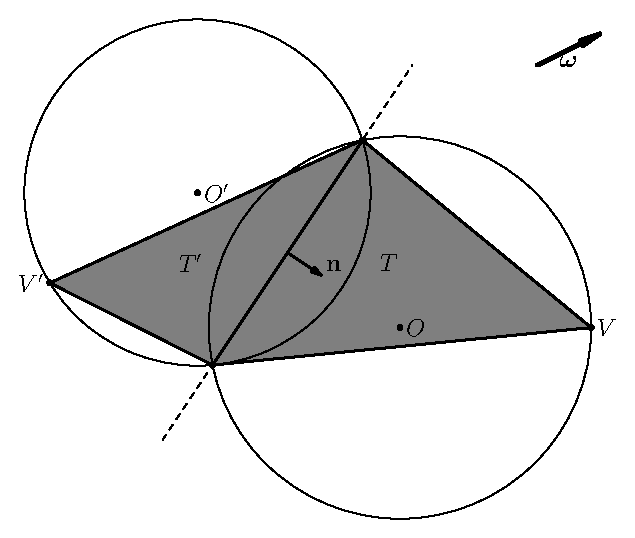
\includegraphics[height=.4\textheight]{spheres-0.eps}
\caption{К доказательству корректности упорядочения для триангуляций Делоне}
\label{fig:spheres}
\end{figure}
\[
V(T) = \frac{1}{3} S \vec n \overrightarrow{MV}, \qquad V(T') = \frac{1}{3} S \vec n \overrightarrow{V'M},
\]
где $S$ --- площадь их общей грани. Суммируя и учитывая $V(T) + V(T') > 0$, получаем
\[
\vec n \overrightarrow{V'V} > 0.
\]

Условие Делоне означает, что расстояние от точки $O$ до $V'$ должно быть больше расстояния от $O$ до $V$. Аналогично для второй сферы:
\[
|OV'| > |OV|, \quad |O'V| > |O'V'|.
\]
Возводя последние соотношения в квадрат, получаем
\[
(\overrightarrow{OV'},\overrightarrow{OV'}) - (\overrightarrow{OV},\overrightarrow{OV}) > 0, \qquad
(\overrightarrow{O'V},\overrightarrow{O'V}) - (\overrightarrow{O'V'},\overrightarrow{O'V'}) > 0
\]
Добавляя и вычитая $(\overrightarrow{OV'},\overrightarrow{OV})$, получаем
\begin{multline*}
0 < (\overrightarrow{OV'},\overrightarrow{OV'}) - (\overrightarrow{OV},\overrightarrow{OV}) =
(\overrightarrow{OV'},\overrightarrow{OV'}) 
-(\overrightarrow{OV'},\overrightarrow{OV})
+(\overrightarrow{OV'},\overrightarrow{OV})
- (\overrightarrow{OV},\overrightarrow{OV}) = \\ =
(\overrightarrow{OV'},\overrightarrow{VV'}) 
+
(\overrightarrow{VV'}, \overrightarrow{OV}) = 
\left(\overrightarrow{VV'}, \frac{\overrightarrow{OV}+ \overrightarrow{OV'}}{2}\right)
\end{multline*}
Аналогично,
\[
\left(\overrightarrow{V'V}, \frac{\overrightarrow{O'V}+ \overrightarrow{O'V'}}{2}\right)  =
\left(\overrightarrow{VV'}, \frac{\overrightarrow{VO'}+ \overrightarrow{V'O'}}{2}\right) 
> 0.
\]
Суммируя данные неравенства, получаем
\begin{equation}
(\overrightarrow{VV'},\overrightarrow{OO'}) > 0.
\label{eq:half}
\end{equation}
Так как точки $O,O'$ (а также $V,V'$) находятся в разных полупространствах, разделенных гранью, условие \eqref{eq:half} показывает, что точки $O$ и $V$ находятся с одной стороны грани, а $O'$ и $V'$ --- с другой. Таким образом, вектор $\overrightarrow{O'O}$ не только коллинеарен $\vec n$, но и сонаправлен с ним. Поэтому условие $T \succ T'$, эквивалентное $\vec \omega \vec n > 0$, эквивалентно $\vec \omega \overrightarrow{O'O} > 0$, что в свою очередь эквивалентно $\pi(T) > \pi(T')$. Полученное противоречие доказывает $T \prec T' \Rightarrow \pi(T) < \pi(T')$.

Используемые строгие неравенства предполагают общее расположение тетраэдров (описанные сферы двух тетраэдров не могут совпадать). Выполнения этого условия можно добиться небольшим возмущением триангуляции. Заметим, что для триангуляции Делоне невозможно образование циклов в отношении $\prec$.


\subsection{Алгоритм для триангуляций общего вида}

Для построения упорядочения $c(T)$ триангуляции общего вида можно воспользоваться модификацией алгоритма Тарьяна \cite{Corman2009} для топологической сортировки, который в свою очередь, является простой модификацией поиска в ширину.

В алгоритме \ref{alg:coloring} используется очередь тетраэдров, заполненная изначально тетраэдрами, у которых все входные грани освещены, то есть теми тетраэдрами, для которых на всех входных гранях задано граничное условие.

На очередном шаге алгоритма из очереди извлекается тетраэдр $T$. Проверяется, присвоен ли номер $c(T_j)$ всем его предшествующим соседям $T_j \prec T$. Если это так, тетраэдру $T$ присваивается номер
\[
c(T) = 1 + \max_{T_j \prec T} c(T_j).
\]
В случае, когда тетраэдр $T$ лежит на границе области, для отсутствующих соседей $T_j$ формально полагается $c(T_j) = 0$. Это позволяет присвоить всем тетраэдрам, которые изначально были в очереди номер $c(T) = 1$. После присвоения номера тетраэдру $T$, в очередь добавляются все следующие за ним тетраэдры $T' \succ T$, которым еще не присвоен номер.

Если хотя бы одному предшествующему соседу $T_j \prec T$ еще не присвоен номер, тетраэдр $T$ возвращается в конец очереди. Данный алгоритм способен определять наличие циклов в отношении $\prec$. Если в триангуляции обнаружен цикл, тетраэдры будут постоянно извлекаться и добавляться в конец очереди. Алгоритмически это можно определить используя счетчик. После добавления нового тетраэдра в очередь счетчик устанавливается равным длине очереди, а при возвращении тетраэдра обратно в очередь, счетчик уменьшается на единицу. Если на очередном шаге алгоритма счетчик обнуляется, это свидетельствует о том, что последние $n$ шагов алгоритма из очереди длины $n$ тетраэдры только извлекались и добавлялись обратно, причем ни одному новому тетраэдру не был присвоен номер. Данный факт свидетельствует о зацикливании алгоритма, а значит граф отношения $\prec$ не является ациклическим. Работа алгоритма проиллюстрирована на рисунке \ref{fig:coloring}.
\begin{figure}[ht!]
\centering
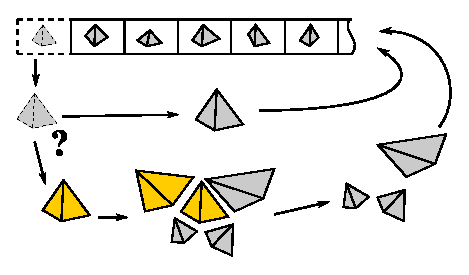
\includegraphics[height=.3\textheight]{coloring.eps}
\caption{Иллюстрация работы алгоритма упорядочения}
\label{fig:coloring}
\end{figure}

\begin{algorithm}[ht!]
\centering
\begin{algorithmic}[1]
\Procedure{Ordering}{}
\State $Q :=$ \Call{InitQueue}{}
\State $cnt := |Q|$
\While {$Q \neq \emptyset$}
\State $T :=$ \Call{Dequeue}{$Q$}
\If {$\forall T' \prec T, c(T') \neq \mathbf{nil}$}
\State $c(T) := 1 + \max_{T' \prec T} c(T')$
\For {$T'' \succ T: c(T'') = \mathbf{nil}$}
\State \Call{Enqueue}{$Q$, $T''$}
\EndFor
\State $cnt := |Q|$
\Else
\State \Call{Enqueue}{$Q$, $T$}
\State $cnt := cnt - 1$;
\EndIf
\If {$cnt < 0$}
\State \textbf{error} В триангуляции обнаружен цикл.
\EndIf
\EndWhile
\EndProcedure
\end{algorithmic}
\caption{Алгоритм упорядочения для произвольной триангуляции}
\label{alg:coloring}
\end{algorithm}

Заметим, что данное упорядочение является оптимальным в том смысле, что каждому тетраэдру $T$ присваивается минимально возможный номер $c(T)$. При этом максимальный номер будет присвоен последнему тетраэдру в самой длинной цепочке зависимых тетраэдров
\[
T_1 \prec T_2 \prec \dots \prec T_n.
\]

\section{Связь минимального порядка $c(T)$ с ярусно-параллельной формой алгоритма}

Если упорядочение $c(T)$ минимально, например, построено с помощью алгоритма \ref{alg:coloring}, то множество всех тетраэдров сетки разбивается на непересекающиеся подмножества
\[
U_k = \left\{T \mid c(T) = k\right\}.
\]
При этом для вычисления решения в каждом тетраэдре $T \in U_k$ достаточно знать решения для каждого тетраэдра $T' \in \bigcup_{j = 1}^{k - 1} U_j$. В частности, решение в $T$ не зависит от решения в тетраэдрах $T''$ с тем же номером $c(T'') = k$. Последнее свойство означает, что решения во всех тетраэдрах из $U_k$ можно находить параллельно.

Заметим, что ациклический граф отношения $\prec$ является также графом зависимостей вычислительного алгоритма, а построенное упорядочение фактически задает ярусно-параллельную его форму \cite{Karpov2014}. По определению, ярусно-параллельной формой называется деление графа на такие множества $V_i$, что для каждой дуги $u \to v, u \in V_j, v \in V_k$ выполняется $j < k$.
В маршевом методе решение вычисляется последовательно для каждого множества $U_k, k = 1, \dots, n$, но в каждом множестве $U_k$ решение может вычисляться параллельно. На рисунке \ref{fig:marching} показаны тетраэдры, в которых решение уже вычислено для различных моментов <<марша>>: в начале, в середине и в конце.

\begin{figure}[ht!]
\centering
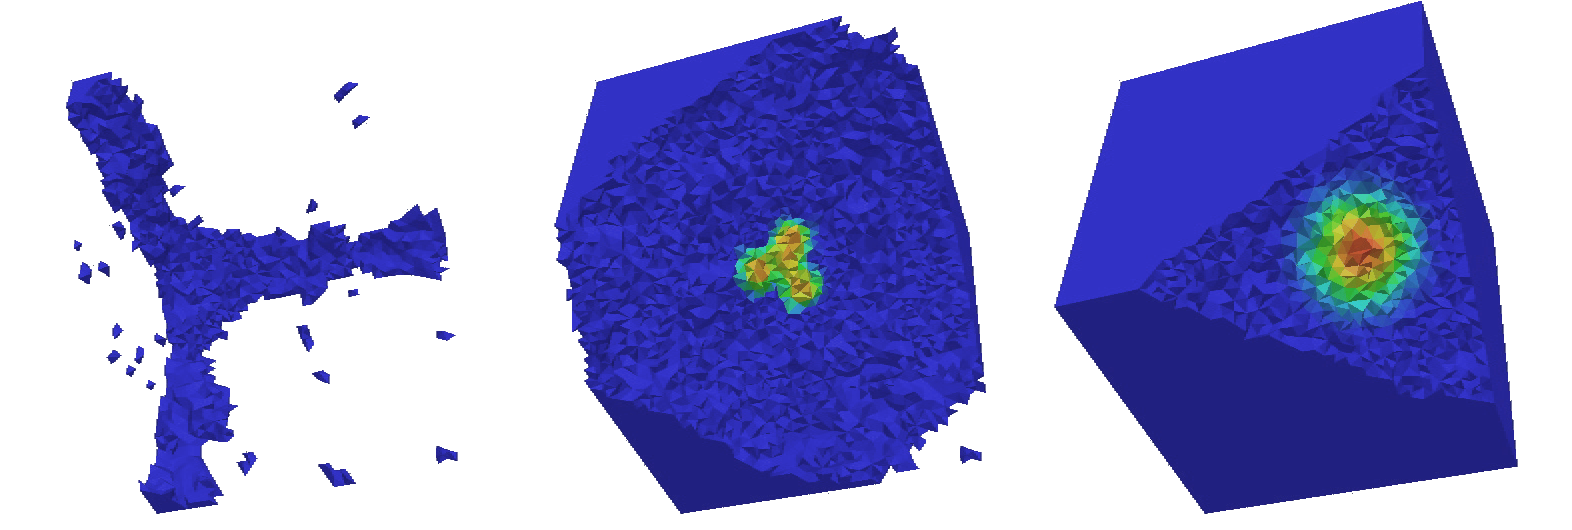
\includegraphics[height=.2\textheight]{123.png}
\caption{Множество тетраэдров с номером $c(T) < k$ для различных $k$}
\label{fig:marching}
\end{figure}

Однако, для параллельной реализации алгоритма требуется учитывать накладные расходы на построение упорядочения $c(T)$. Алгоритм упорядочения существенно последователен, поэтому выигрыш от распараллеливания возможен лишь в двух случаях
\begin{itemize}
\item решение задачи в каждом тетраэдре ресурсоемко, например, одновременно решается уравнение переноса для большого числа частот;
\item производится многократное решение уравнения переноса, например, на протяжении большого числа шагов по времени.
\end{itemize}
В последнем случае для каждого направления переноса необходимо хранить упорядочение $c(T)$. К тому же, между шагами по времени не должна изменяться расчетная сетка. Последнее обстоятельство сильно ограничивает применимость параллельного алгоритма на подвижных сетках.           % Глава 3
\chapter{Распределенный метод длинных характеристик}

Метод длинных характеристик является наиболее точным методом решения уравнения переноса излучения. Метод основывается на точном решении уравнения переноса в каждом направлении.

Уравнение переноса 
\[
(\vec \Omega \nabla) I(\vec r, \vec \Omega) + \varkappa(\vec r, \vec \Omega) I(\vec r, \vec \Omega) = \varkappa(\vec r, \vec \Omega) I_\text{p}(\vec r, \vec \Omega)
\]
вдоль характеристики
$
\vec r - \vec r_0 = \vec \Omega (s - s_0)
$
превращается в обыкновенное дифференциальное уравнение
\[
\frac{dI(s)}{ds} + \varkappa(s) I(s) = \varkappa(s) I_\text{p}(s)
\]
и может быть легко проинтегрировано точно:
\begin{equation}
I(s) = I(s_0) e^{-\tau(s_0, s)} + \int_{s_0}^s \varkappa(\xi) I_\text{p}(\xi)
e^{-\tau(\xi,s)} d\xi.
\label{eq:exact}
\end{equation}
В последнем выражении $\tau(a,b) = \int_a^b \varkappa(s) ds$ --- оптическая длина отрезка характеристики от точки $s = a$ до точки $s = b$.

Соотношение \eqref{eq:exact} лежит в основе метода длинных характеристик. В отличие от метода коротких характеристик, где характеристика выпускается из узла до входной грани тетраэдра, в методе длинных характеристик она выпускается до границы расчетной области, см. рисунок \ref{fig:lcm}.
\begin{figure}[ht!]
\centering
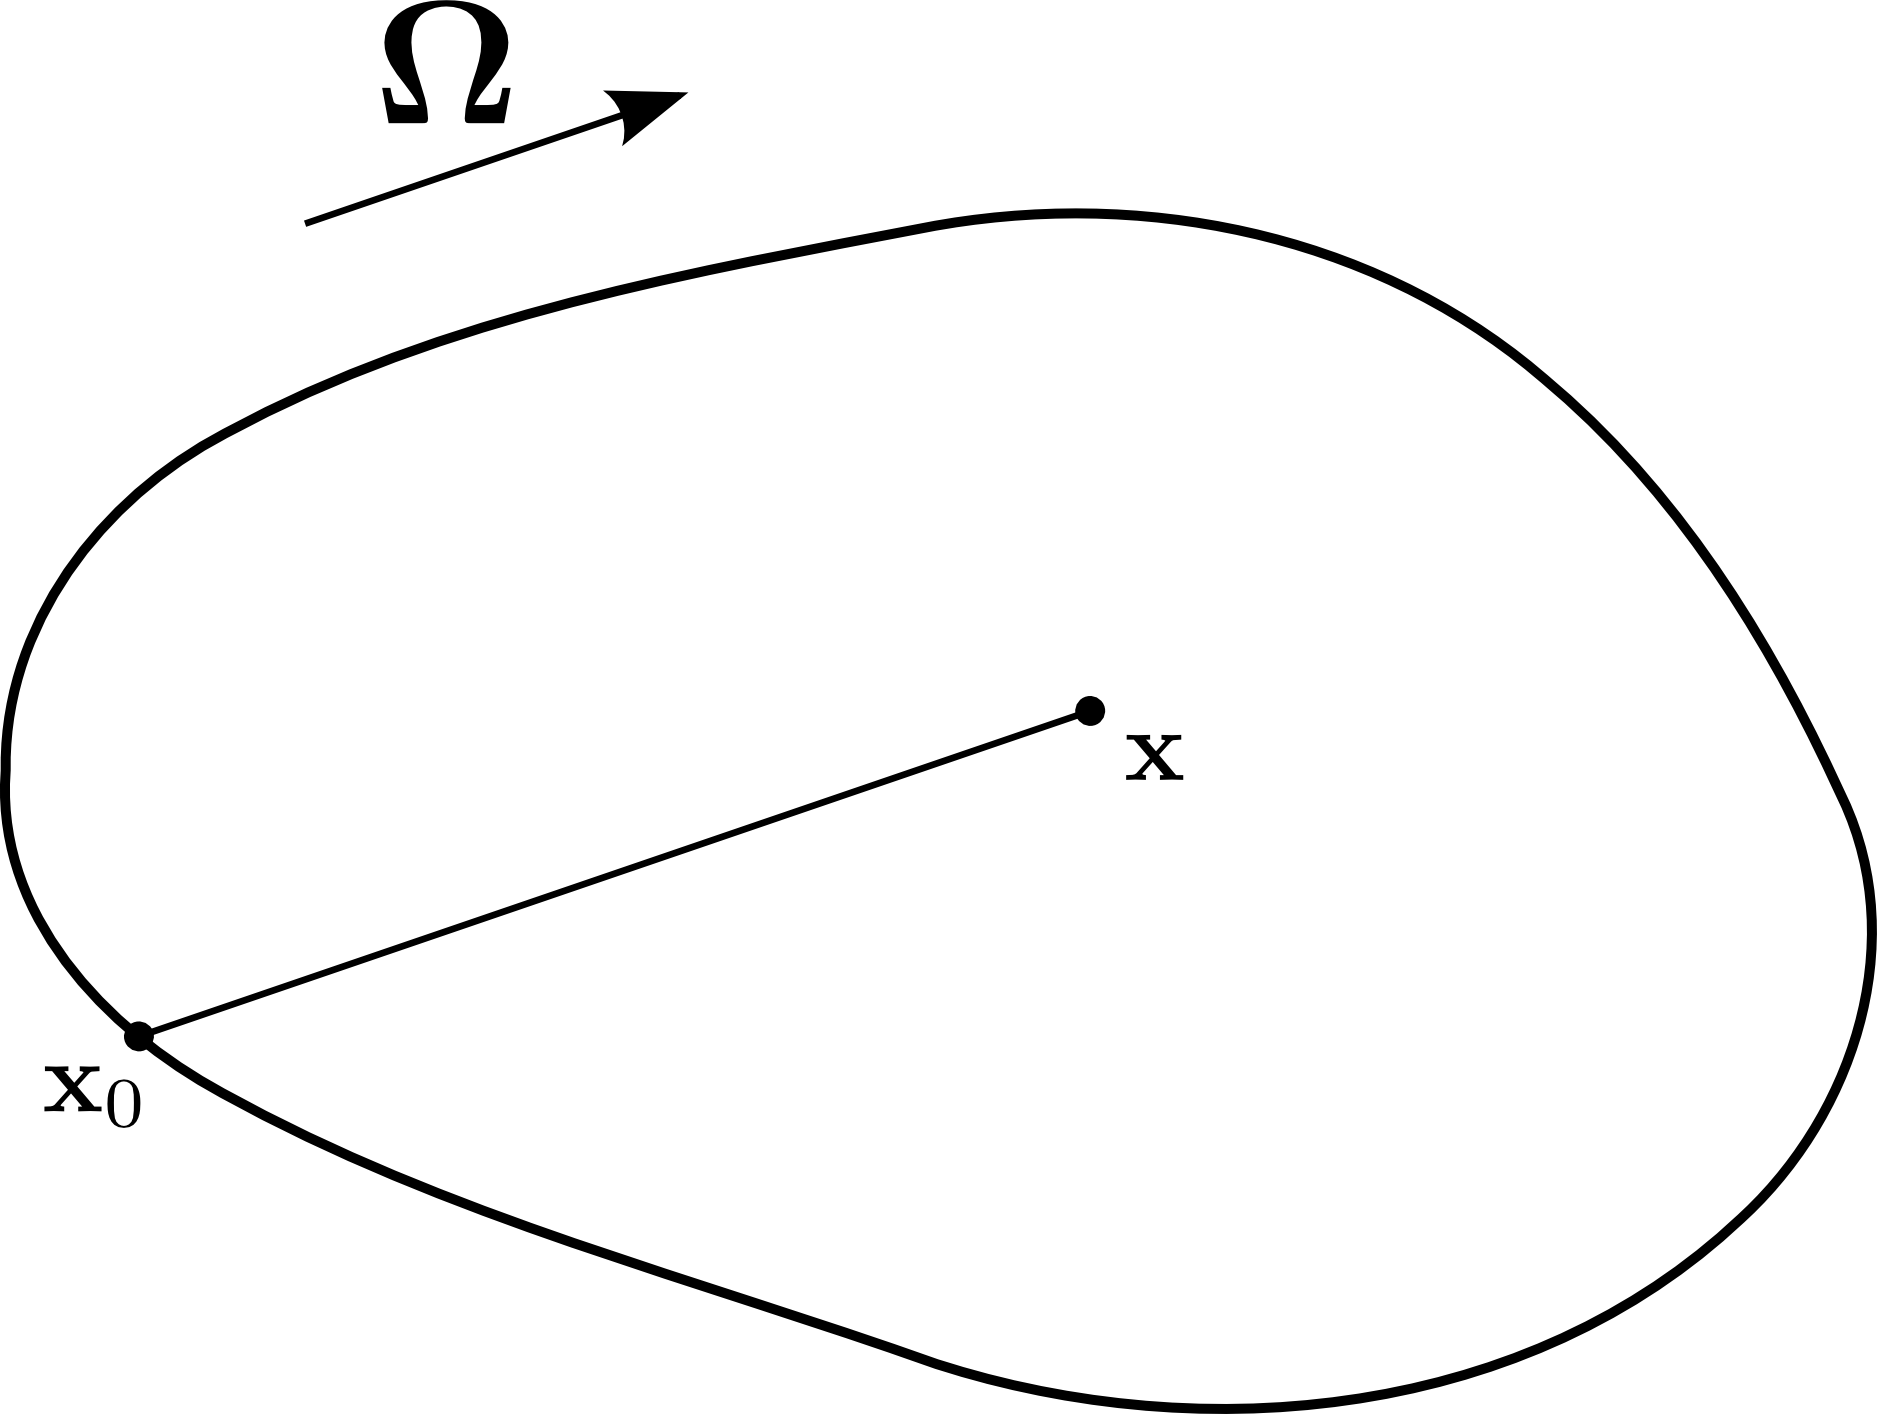
\includegraphics[height=0.25\textheight]{lcm.png}
\caption{Нахождение решения методом длинных характеристик}
\label{fig:lcm}
\end{figure}

\section{Функция Грина для задачи переноса излучения}

Заметим, что соотношение \eqref{eq:exact} представляет собой выражение функции Грина, так как связывает решение в точке $I(\vec r, \vec \Omega)$ с граничным условием $I(\vec r_0, \vec \Omega), \vec r_0 \in \partial G$.

Введем обозначения $\alpha(s_0, s)$ и $\beta(s_0, s)$ 
\begin{gather*}
\alpha(s_0, s) = e^{-\tau(s_0, s)}\\
\beta(s_0, s) = \int\limits_{s_0}^s \varkappa(\xi) I_\text{p}(\xi) \alpha(\xi, s) d\xi.
\end{gather*}

В этих обозначениях функция Грина записывается в виде
\begin{equation}
I(s) = \alpha(s_0, s) I(s_0) + \beta(s_0, s).
\label{eq:connection}
\end{equation}
При $s > s_0$ для величин $\alpha(s_0, s), \beta(s_0, s)$ справедливо
\begin{equation}
\begin{gathered}
0 < \alpha(s_0, s) \leqslant 1\\
0 \leqslant \beta(s_0, s) \leqslant \max_{\xi \in [s_0, s]} I_\text{p}(\xi)
\cdot \int_{s_0}^s \varkappa(\xi) e^{-\tau(\xi, s)} d\xi = \\ =
\max_{\xi \in [s_0, s]} I_\text{p}(\xi)
\cdot \int_{0}^{\tau(s_0,s)} e^{-u} du =
(1 - \alpha(s_0, s))\max_{\xi \in [s_0, s]} I_\text{p}(\xi).
\end{gathered}
\label{eq:limits}
\end{equation}
С учетом \eqref{eq:limits} для $I(s)$ верен принцип максимума
\[
I(s) \leqslant \alpha(s_0, s) I(s_0) + (1 - \alpha(s_0, s))\max_{\xi \in [s_0, s]} I_\text{p}(\xi) \leqslant \max\left(I(s_0); \max_{\xi \in [s_0, s]} I_\text{p}(\xi)\right).
\]

Фактически, функция Грина задается лишь двумя коэффициентами для каждой точки $\vec r$ и направления $\vec \Omega$. В численном методе точка $\vec r_0$ не является узлом сетки, а значение $I(\vec r_0, \vec \Omega)$ находится интерполяцией интенсивности по грани, содержащей точку $\vec r_0$. При этом численная функция Грина дополнительно задается коэффициентами интерполяции и номерами вершин грани.

Для сравнения, численная функция Грина, построенная в методе коротких характеристик, зависит от большого числа узлов на границе. Увеличение шаблона вызвано в этом методе многократной интерполяцией.

\subsection{Трассировочное соотношение}

Для практического вычисления коэффициентов $\alpha(s_0, s)$ и $\beta(s_0, s)$ удобно пользоваться следующим соотношением при $s_0 \leq s_1 \leq s$:
\[
\alpha(s_0, s) = e^{-\tau(s_0, s)} = 
e^{-\tau(s_0, s_1) -\tau(s_1, s)} = 
\alpha(s_0, s_1)\alpha(s_1, s),
\]
следующим из аддитивности оптической длины.

Для $\beta(s_0, s)$ справедливо
\begin{multline*}
\beta(s_0, s) = 
\int\limits_{s_0}^s \varkappa(\xi) I_\text{p}(\xi) \alpha(\xi, s) d\xi = \\ =
\int\limits_{s_0}^{s_1} \varkappa(\xi) I_\text{p}(\xi) \alpha(\xi, s) d\xi +
\int\limits_{s_1}^s \varkappa(\xi) I_\text{p}(\xi) \alpha(\xi, s) d\xi = \\ =
\int\limits_{s_0}^{s_1} \varkappa(\xi) I_\text{p}(\xi) \alpha(\xi, s_1) \alpha(s_1, s) d\xi +
\int\limits_{s_1}^s \varkappa(\xi) I_\text{p}(\xi) \alpha(\xi, s) d\xi = \\
= \beta(s_0, s_1) \alpha(s_1, s) + \beta(s_1, s).
\end{multline*}

Фактически, соотношения между коэффициентами $\alpha, \beta$ следуют из принципа Гюйгенса
\begin{multline*}
I(s) = \alpha(s_1, s) I(s_1) + \beta(s_1, s) = \\ =
\alpha(s_1, s) \Big(\alpha(s_0, s_1) I(s_0) + \beta(s_0, s_1)\Big) + \beta(s_1, s)
= \\ =
\alpha(s_0, s_1)\alpha(s_1, s) I(s_0) + \beta(s_0, s_1)\alpha(s_1, s) + \beta(s_1, s).
\end{multline*}

Будем называть соотношения
\begin{equation}
\begin{gathered}
\alpha(s_0, s) = \alpha(s_0, s_1)\alpha(s_1, s),\\
\beta(s_0, s) = \beta(s_0, s_1) \alpha(s_1, s) + \beta(s_1, s)
\end{gathered}
\end{equation}
трассировочными. С помощью них удобно вычислять коэффициенты $\alpha(s_0, s), \beta(s_0, s)$, двигаясь вдоль характеристики по тетраэдрам триангуляции (см. рисунок \ref{fig:trace}). При переходе от коэффициентов $\alpha(s_1, s), \beta(s_1, s)$ к коэффициентам $\alpha(s_0, s), \beta(s_0, s)$ достаточно знать только значения
$\alpha(s_0, s_1), \beta(s_0, s_1)$. Для однородных значений $\varkappa, I_\text{p}$ в тетраэдре,
\[
\alpha(s_0, s_1) = e^{-\varkappa (s_1 - s_0)},\qquad
\beta(s_0, s_1) = \big(1 - \alpha(s_0, s_1)\big) I_\text{p}.
\]
\begin{figure}[ht!]
\centering
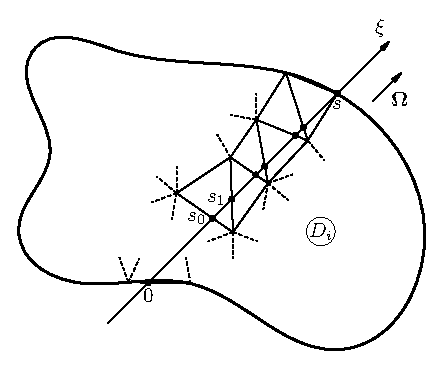
\includegraphics[width=.4\textwidth]{trace-0.eps}
\caption{Трассировка луча по триангуляции}
\label{fig:trace}
\end{figure}

\section{Устойчивая трассировки луча}

Рассмотрим процесс трассировки луча из точки $\vec r$. Трассировка начинается в тетраэдре $T$, содержащем точку $\vec r - 0 \vec \Omega$. Для каждой треугольной грани $Q = \operatorname{conv}(r_1, r_2, r_3)$ тетраэдра находятся барицентрические координаты $\gamma_k$ точки пересечения $\vec r^* = \sum_{k=1}^3 \gamma_k \vec r_k$ плоскости грани с лучом $\vec r - \vec \Omega s$.  Находится грань, для которой все барицентрические координаты $\gamma_k$ неотрицательны. Для этой грани $\vec r^* \in Q$. Псевдокод данной процедуры изложен в алгоритме \ref{alg:traceelem}  
\begin{algorithm}[ht!]
\centering
\begin{algorithmic}[1]
\Function{TraceElement}{$e$, $P \in e, \vec \omega$}
%\State $P := $ \Call{ShiftToStable}{$e, P$}
\For{каждой грани $f \in e$}
\State $(\vec r_1, \vec r_2, \vec r_3) := $ \Call{VertexCoordinates}{$f$}
\State $\triangleright$  Решить
$(
\vec r_P - \ell \vec \omega - \vec r_1,
\vec r_2 - \vec r_1,
\vec r_3 - \vec r_1
) = 0$ относительно $\ell$
\If{$(\vec \omega, \vec r_2 - \vec r_1, \vec r_3 - \vec r_1) = 0$}
\State $\mu(f) := \infty$
\State \textbf{continue} \Comment Перейти к следующей грани
\EndIf
\State $\ell := 
\dfrac{(\vec r_P - \vec r_1, \vec r_2 - \vec r_1, \vec r_3 - \vec r_1)}
{(\vec \omega, \vec r_2 - \vec r_1, \vec r_3 - \vec r_1)}$
\If{$\ell < 0$}
\State $\mu(f) := \infty$
\State \textbf{continue} \Comment Перейти к следующей грани
\EndIf
\State $\vec r_Q := \vec r_P - \ell \vec \omega$
\State $\vec\gamma(f) = $ \Call{BarycentricCoordinates}{$f, Q$}
\State $\mu(f) := \sum_{k}|\gamma_k(f)|$
\State $\pi(f) := Q$
\EndFor
\State $f := \operatorname{argmin} \mu(f)$
\State\Return{$\pi(f), f, (\vec\omega, \vec r_Q - \vec r_P), \vec \gamma(f)$}
\EndFunction
\end{algorithmic}
\caption{Алгоритм трассировки в элементе}
\label{alg:traceelem}
\end{algorithm}

После прохождения лучом точки $\vec r^*$, трассируемый луч переходит в точку $\vec r^*$ и в тетраэдр $T'$, граничащий с $T$ по грани $Q = T \cap T'$.  Трассировка заканчивается, когда грань $Q$ очередного тетраэдра является граничной.

Параллельно с трассировкой тетраэдров производится вычисление $\alpha(s_0, s), \beta(s_0, s)$. В начале трассировке величины $\alpha, \beta$ инициализируются значениями $\alpha = 1, \beta = 0$.
При прохождении очередного тетраэдра, вычисляются коэффициенты $\tilde \alpha = \alpha(s_0, s_1)$ и $\tilde \beta = \beta(s_0, s_1)$ и производится обновление по правилу
\[\begin{aligned}
\beta &:= \beta + \tilde \beta \alpha\\
\alpha &:= \alpha \tilde \alpha.
\end{aligned}
\]
При завершении трассировки луча переменные $\alpha, \beta$ содержат значения $\alpha(0, s)$ и $\beta(0, s)$.

При практической реализации алгоритма \ref{alg:traceelem} возникает проблема, вызванная ошибками округления. Трассировка может зациклиться, если луч проходит вблизи ребра или вершины.

Введем определения входной и выходной грани, устойчивые к ошибках округлений.
Если $\mathbf n$ --- нормаль к грани, а $\boldsymbol \Omega$ --- направление излучения, то в случае
%\newpage
\begin{itemize}
\item если $(\mathbf n \boldsymbol \Omega) < -\epsilon$, то грань называется входной (луч входит в тетраэдр);
\item если $(\mathbf n \boldsymbol \Omega) > \phantom{-}\epsilon$, то грань называется выходной (луч выходит из тетраэдра);
\item иначе, грань называется касательной.
\end{itemize}
В этом определении $\epsilon \ll 1$ --- малое число. В реализации использовалось $\epsilon = 10^{-6}$.

Рассмотрим выпуклый многогранник $P_1P_2\dots P_n$ и точку $Q$ внутри него. Выпустим из точки $Q$ 
луч в направлении $-\vec\omega$. Этот луч выйдет через некоторую грань $f$ многогранника $T$.

Чтобы луч не выходил через касательную грань достаточно сместить точку $Q$ внутрь многогранника 
$T$. Справедлива следующая лемма:
\newtheorem{lemma}{Лемма}
\begin{lemma}[Об устойчивой трассировке]
Если точка $Q$ в многограннике $T = P_1P_2\dots P_n$ находится на расстоянии более $\delta 
\equiv \epsilon \cdot d(T)$ от каждой грани, то луч из точки $Q$ в направлении
$-\boldsymbol \omega$ выйдет через входную грань многогранника. Здесь $d(T)$ --- диаметр 
многогранника $T$, то есть максимальное расстояние между двумя его точками.
\end{lemma}
\begin{proof}[Доказательство]
Пусть $S$ --- точка грани $f$ многогранника (см. рисунок \ref{fig:touch}), через которую луч выходит из него.
\begin{figure}[ht!]
\centering
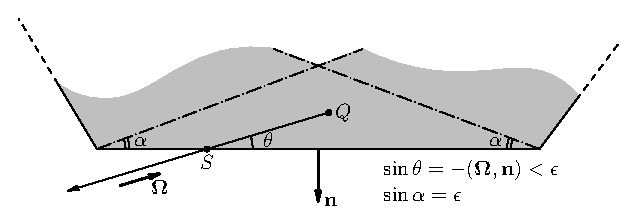
\includegraphics[width=.8\textwidth]{shift-0}
\caption{Точка $Q$ и выходящий из нее касательный луч. Точка $Q$ необходимо должна принадлежать 
серой области}
\label{fig:touch}
\end{figure}

Предположим, что грань является касательной к лучу. Это означает, что $\sin \theta = -(\vec \omega, 
\vec n) \leqslant \epsilon$. Поскольку обе точки $S,Q$ принадлежат $T$, то $|SQ| \leq d(T)$. 
Следовательно, высота, опущенная из $Q$ на грань $f$ не может иметь длину более $\sin \theta \cdot 
d(T) \leq \epsilon \cdot d(T) \equiv \delta$. Следовательно условие $\rho(Q, f) > \delta$ 
гарантирует, что луч не может выйти через грань $f$ так, чтобы быть к ней касательным. Обобщая это 
на все грани многогранника $T$, получаем утверждение леммы.
\end{proof}

Условие данной леммы можно усилить: $\rho(Q, f) > \delta$ является достаточным, но не необходимым. 
Однако, удовлетворить этому условию намного проще, чем точному условию (на рисунке
\ref{fig:forb} точное запрещенное множество закрашено серым цветом, а пунктиром обозначено множество из леммы).
\begin{figure}[ht!]
\centering
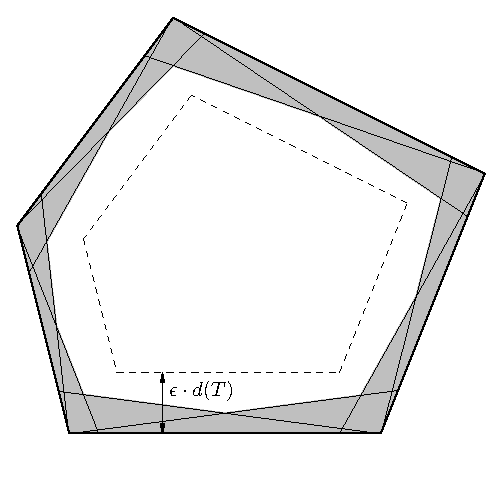
\includegraphics[width=.5\textwidth]{shift-1}%
\caption{Исходный многогранник, запрещенная область (серая) и область из леммы. Для трехмерного 
случая реальная запрещенная область имеет достаточно сложную форму}
\label{fig:forb}
\end{figure}

\begin{figure}[ht!]
\centering
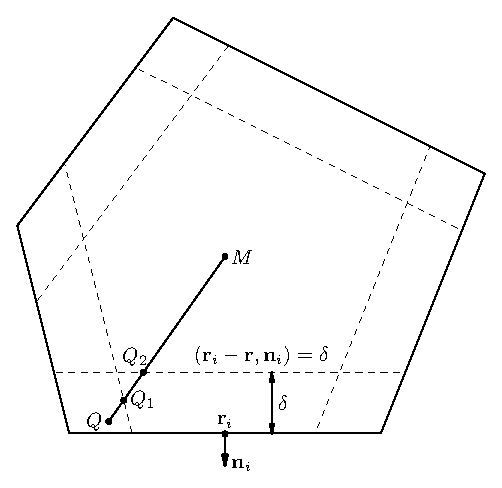
\includegraphics[width=.5\textwidth]{shift-2}%
\caption{Иллюстрация процедуры сдвига точки $Q$ в допустимое множество из леммы}
\end{figure}
Однако, простота этого условия порождает простую процедуру сдвига точки в допустимое множество (при 
условии, что центр масс $M$ многогранника сам лежит в допустимом множестве). Рассмотрим отрезок, 
соединяющий точки $M$ и $Q$, а также все плоскости, содержащие грани многогранника. Пусть каждая из 
этих плоскостей задана уравнением $(\vec r_i - \vec r, \vec n_i) = 0$. Несложно заметить, что 
условия леммы требуют выполнения соотношений $(\vec r_i - \vec r_Q, \vec n_i) > \delta$ для каждой 
$i$-й грани многогранника. Дополнительно требуя, чтобы новая точка $Q_i$ лежала на отрезке $QM$, 
получаем соотношения
\begin{gather*}
\vec r_{Q'} = \lambda \vec r_{Q} + (1 - \lambda) \vec r_{M}, \quad \lambda \in [0,1]\\
\lambda \rightarrow \max_{(\vec r_i - \vec r_{Q_i}, \vec n_i) > \delta}
\end{gather*}
Данная система линейных неравенств на $\lambda$ может быть легко решена последовательно для каждой грани, с выбором минимального $\lambda = \min_i \lambda_i$, см. алгоритм \ref{alg:shift}.

\begin{algorithm}[ht!]
\centering
\begin{algorithmic}[1]
\Function{ShiftToStable}{$e, Q$}
\State $\lambda := 1$
\State $\delta := \epsilon \cdot d(e)$
\State $\vec r_M := $ \Call{MassCenter}{$e$}
\For{каждой грани $f \in e$}
\State $(\vec r_i, \dots) := $ \Call{VertexCoordinates}{$f$}
\Comment Выбрать точку $\vec r_i \in f$
\State $\vec n_i := $ \Call{FaceNormal}{$f$}
\State $\vec r_{Q'} = \lambda \vec r_Q + (1 - \lambda) \vec r_{M}$
\If{$(\vec r_i - \vec r_{Q'}, \vec n_i) > \delta$}
\State \textbf{continue} \Comment Перейти к следующей грани
\Else
\State $\triangleright$ Найти точку пересечения отрезка $QM$ и плоскости
\State $\lambda := \frac{\delta - (\vec r_i - \vec r_M, \vec n_i)}
{(\vec r_Q - \vec r_M, \vec n_i)}$
\EndIf
\EndFor
\State $\vec r_{Q'} = \lambda \vec r_Q + (1 - \lambda) \vec r_{M}$
\State\Return{$Q'$}
\EndFunction
\end{algorithmic}
\caption{Алгоритм смещения точки в элементе}
\label{alg:shift}
\end{algorithm}

Заметим, что при использовании сдвига, длина отрезка характеристики в многограннике не меньше $\delta$, а следовательно при прохождении очередного тетраэдра точка продвигается в направлении $-\vec \Omega$ хотя бы на расстояние $\delta$.
Трассировка области с вычислением коэффициентов $\alpha, \beta$ представлена в алгоритме \ref{alg:tracedom}.

\begin{algorithm}[ht!]
\centering
\begin{algorithmic}[1]
\Function{TraceDomain}{$\mathcal{T}, P \in D, \vec\omega$}
\State $\alpha := 1$
\State $\beta := 0$
\State $e := $ \Call{ContainingElement}{$\mathcal{T}, P$}
\Repeat
\State $(Q, f. \ell, \vec\gamma) :=$ \Call{TraceElement}{$e, P, \vec \omega$}
\State $\Delta := \ell \varkappa(e) $
\Comment{Оптическая толщина элемента $e$}
\State $q := e^{-\Delta}$
\State $\beta := \beta + (1 - q)\alpha I_e(e)$
\State $\alpha := q\alpha$
\State $e := $ \Call{NeighbourOverFace}{$\mathcal{T}, e, f$}
\State $P := Q$
\Until{\textbf{not} \Call{IsValidElement}{$e$}}
\State\Return{$\alpha, \beta, \vec \gamma, f$}
\EndFunction
\end{algorithmic}
\caption{Алгоритм трассировки в триангуляции $\mathcal{T}$ области}
\label{alg:tracedom}
\end{algorithm}

\section{Распределенный метод}

Реализация метода длинных характеристик осложняется, если вычислительная область разбита на подобласти. Обычно каждая подобласть принадлежит своему вычислительному процессу и трассировка характеристики становится сложной коллективной операцией.

Заметим, что формула \eqref{eq:connection} позволяет не только вычислить неизвестное значение $I(s)$ через известное значение $I(s_0)$, но и просто связать
линейным соотношением два значения интенсивности в двух точках на одном луче.
Если интенсивность излучения каким-то образом оказалась известной на границе вычислительных подобластей, то трассировку лучей достаточно провести в каждой подобласти независимо от других. В этом случае точка $\vec r_0$ --- это точка, в которой характеристика пересекает границу \emph{подобласти}, а не всей вычислительной области (см. рис. \ref{fig:mcm}).

\begin{figure}[ht]
\centering
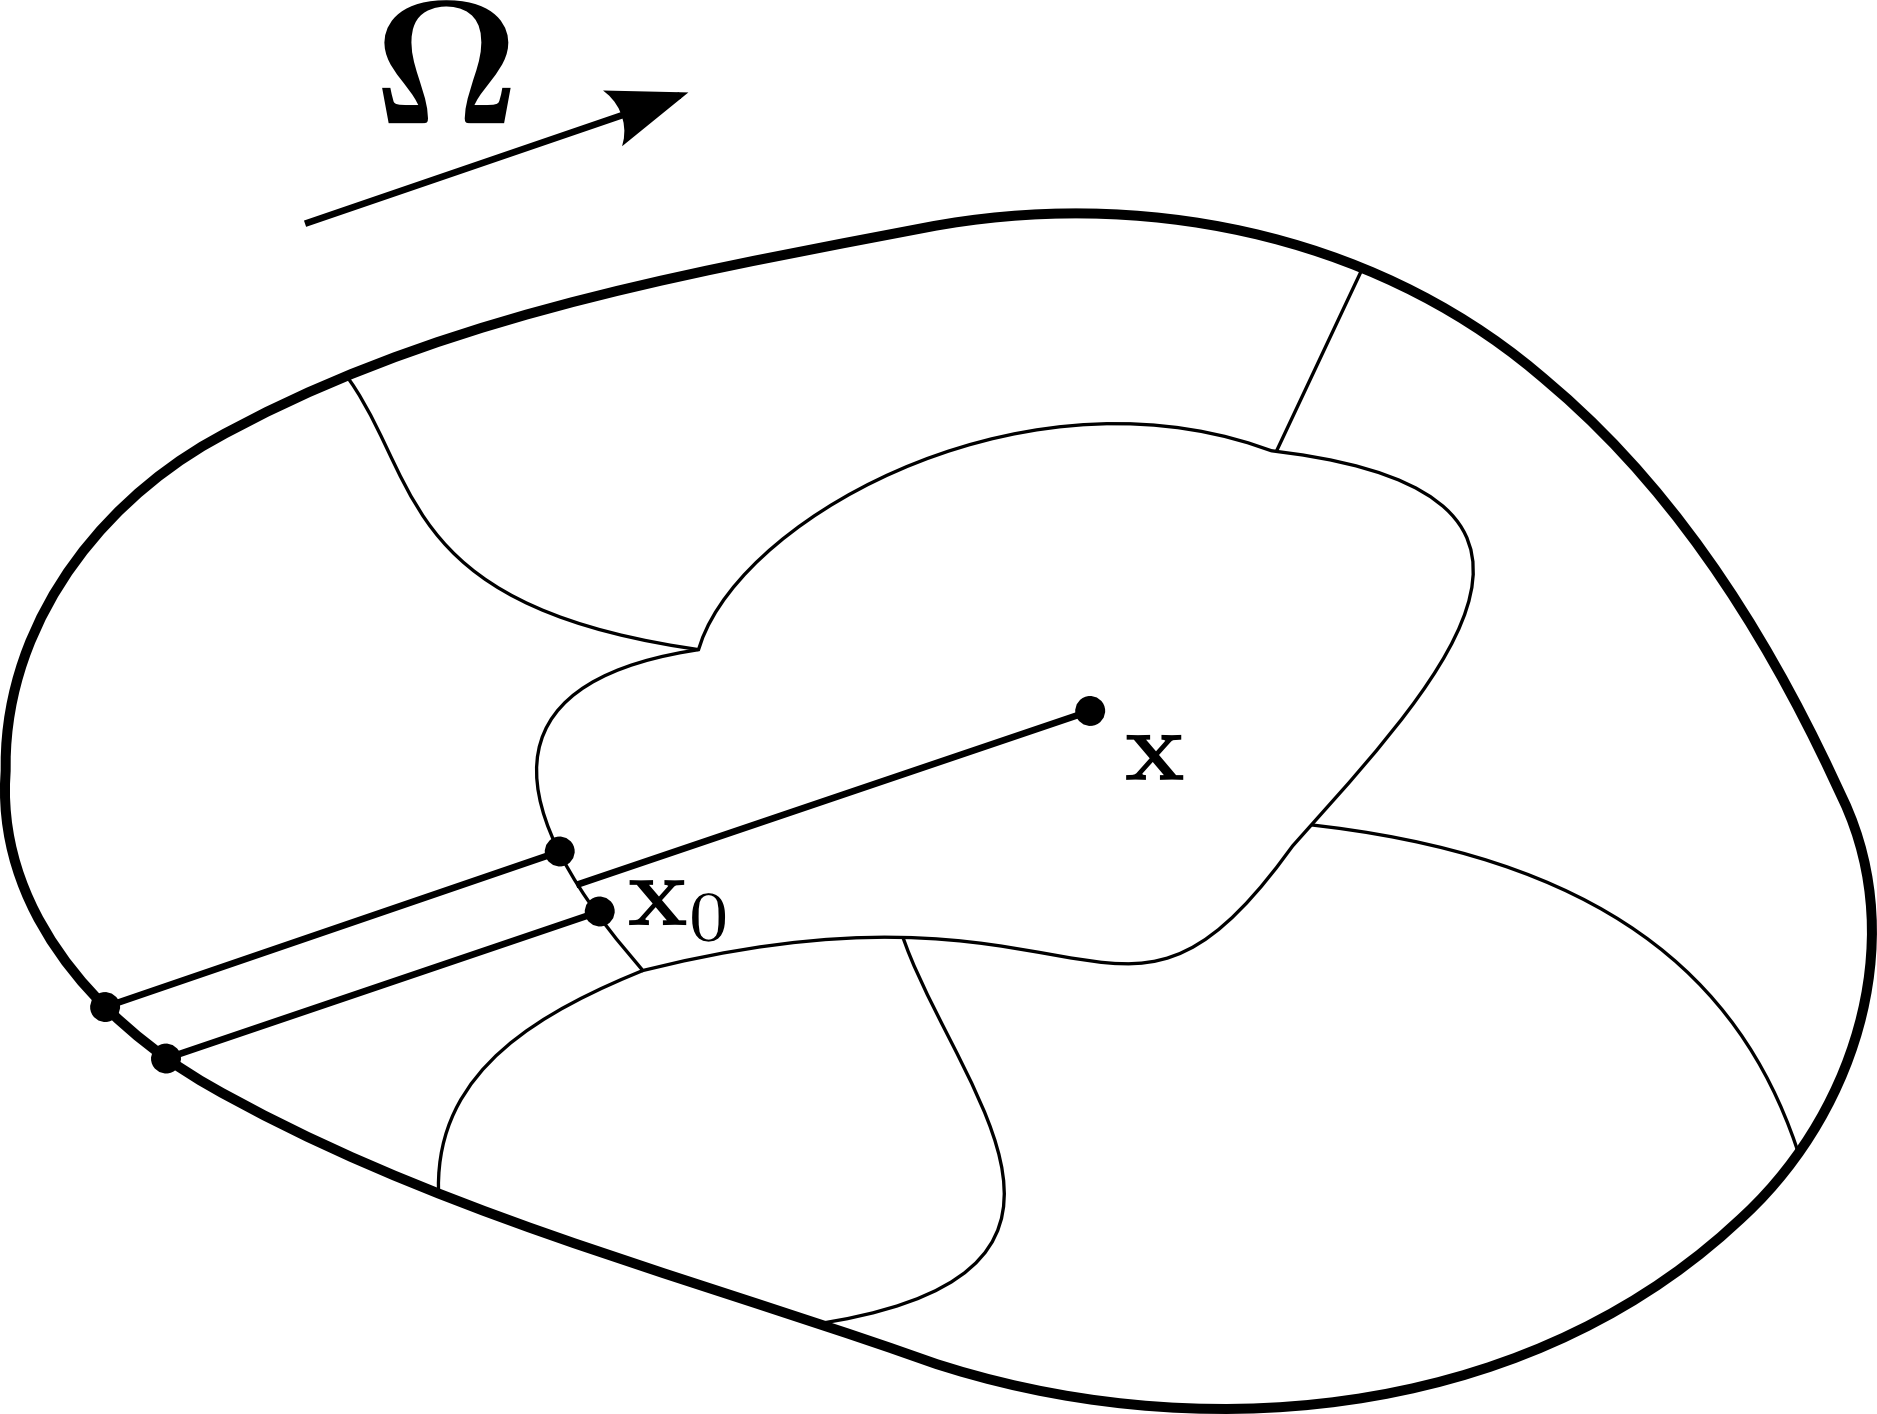
\includegraphics[height=0.3\textheight]{mcm.png}
\caption{Трассировка луча до границы подобласти}
\label{fig:mcm}
\end{figure}

Предположим, что границы подобластей проходят по граням тэтраэдральной сетки, построенной в области. Зафиксируем направление $\vec \Omega$. Будем говорить, что узел сетки (вершина тетраэдра) c координатой $\vec r$ принадлежит подобласти, если точка $\vec r - 0 \vec\Omega$ лежит в подобласти. Если таких подобластей несколько, например, если вектор $\vec \Omega$ лежит в плоскости грани, разделяющей подобласти, выберем подобласть с минимальным номером. Заметим, что определенное таким образом отношение принадлежности зависит не только от геометрических параметров сетки, но и от направления $\vec \Omega$ также. Если узел не принадлежит ни одной подобласти, будем говорить, что он принадлежит \emph{внешней} подобласти, то есть $\mathbb R^3 \setminus G$. Заметим, что интенсивность в граничных узлах, принадлежащих внешней подобласти задана граничными условиями.

Для каждого граничного узла с координатой $\vec r$, принадлежащего подобласти $D_i \subset G$ выпустим характеристику до пересечения с границей подобласти $\partial D_i$. В общем случае, характеристика выйдет из области через некоторую грань $f$ в точке $\vec r_0 = \vec r - \vec \Omega s$. 
Тогда пользуясь соотношением \eqref{eq:connection} заключаем, что
\[
I(\vec r) = \alpha(0, s) I(\vec r_0) + \beta(0, s).
\]
Однако, точка $\vec r$ является узлом расчетной сетки, а точка $\vec r_0$ в общем случае --- нет. Вычислим $I(\vec r_0)$ приближенно интерполяцией интенсивности по вершинам грани $f$
\[
I(\vec r_0) \approx \sum_{j=1}^F \gamma_j I(\vec r_j),
\]
где $F$ --- число вершин грани $f$ (для тетраэдральных сеток $F = 3$), а $\vec r_j$ --- координаты вершин этой грани, которые, в отличие от $\vec r_0$, являются узлами вычислительной сетки. Величины $\gamma_j$ являются обобщенными (для $F > 3$) барицентрическими координатами точки $\vec r_0$ в грани $f$. При этом $\sum_{j=1}^F \gamma_j = 1$.

Таким образом, получается система линейных уравнений, в которые входят значения интенсивности только на границах подобластей, и не входят значения внутри подобластей. Уравнения записаны для каждого граничного узла, принадлежащего некоторой вычислительной подобласти. В узлах, принадлежащих внешней подобласти интенсивность уже задана граничными условиями.

Отметим, что данная система уравнений имеет вид
\begin{equation}
I(\vec r) - \sum_{j=1}^K \gamma_j \alpha(0, s) I(\vec r_j) = \beta(0, s)
\label{eq:slae}
\end{equation}
и имеет диагональное преобладание, поскольку на диагонали стоит коэффициент $1$, а сумма модулей внедиагональных коэффициентов не превосходит $1 - \alpha(0, s) < 1$ некоторые из неизвестных $I(\vec r_j)$ могли быть исключены, если в $\vec r_j$ задано граничное условие).

После коллективного решения системы в узлах на границах подобластей становится известными значения интенсивности. Далее, выпуская характеристики из внутренних точек подобластей восстанавливается решение в каждом узле каждой подобласти всей расчетной области. Эта операция не является коллективной и проводится автономно в каждой подобласти. Также она является самой трудоемкой.

Необходимо подчеркнуть, что решение, полученное данным методом отличается от решения, полученного методом длинных характеристик. В частности, решение зависит от способа декомпозиции на подобласти. Предельный случай декомпозиции области на одну подобласть соответствует методу длинных характеристик, а гипотетический случай декомпозиции на отдельные тетраэдры приводит к методу, где характеристика выпускается от одной грани \emph{тетраэдра} до другой его грани, то есть интерполяция производится на каждой грани, а не только на границе подобласти, как в предлагаемом методе. При этом метод вырождается в метод коротких характеристик. Увеличение количества областей приводит к более частой интерполяции, которая, в свою очередь, вызывает численную диффузию луча. С другой стороны, при этом средняя длина трассируемых лучей уменьшается, что существенно снижает время работы алгоритма.

\section{Параллельная реализация вычислительного алгоритма}

Уравнение переноса решается в некотором наборе направлений. В качестве такого набора были выбраны узлы $\boldsymbol{\omega}_k$ квадратурной формулы для сферы Лебедева 

Для каждого направления $\vec \Omega$ граничные узлы каждой вычислительной подобласти разбиваются на те, которые ей принадлежат (в смысле определения, данного выше) и которые не принадлежат. Из тех, что принадлежат производится трассировка лучей вдоль направления $-\vec \Omega$ до пересечения с границей подобласти алгоритмом \ref{alg:tracedom}.

Таким образом, на каждый процесс формирует в своей подобласти часть общей системы уравнений, в которые входят неизвестные значения интенсивности на границе подобласти.
Далее эта система собирается воедино на одном из процессов, где решается прямым методом для разреженных матриц. Выбор такого метода вместо итерационного обусловлен двумя факторами. Во-первых, размер системы существенно меньше общего количества узлов сетки, так как неизвестные находятся лишь на границах подобластей. Во-вторых, матрицу системы можно превратить в близкую к треугольной, если упорядочить неизвестные по значению их проекции на луч $\vec \Omega$.

Чтобы эффективно использовать остальные процессы, пока на одном из них происходит решение системы, направления обрабатываются не по одному, а по несколько за раз. Это позволяет загрузить все процессы решением систем линейных уравнений, причем каждый процесс будет решать систему для своего направления.

Алгоритм решения состоит из следующих этапов:
\begin{enumerate}
\item Выбирается очередной набор направлений по одному на процесс.
\item Каждый процесс определяет принадлежащие ему точки и производит трассировку от границ в каждом направлении из набора.
\item На каждом процессе собирается система уравнений для его направления из набора.
\item Система решается на каждом процессе и полученное решение рассылается по всем процессам. После этого на каждом процессе становятся известны значения интенсивности на границе его подобласти.
\item В каждой подобласти производится вычисление решения во всех внутренних узлах автономно от остальных процессов.
\item Если остались направления, в которых решение еще не строилось, алгоритм повторяется с первого пункта.
\end{enumerate}

Так как пятый этап алгоритма самый трудоемкий, он был реализован с использованием графических ускорителей. Это позволило не только сократить время расчета задачи, но и произвести перекрытие подготовительных этапов (2-4), производимых на центральном процессоре с этапом 5, производимым на графическом ускорителе (см. рис. \ref{fig:timeline})
\begin{figure}[ht!]
\centering
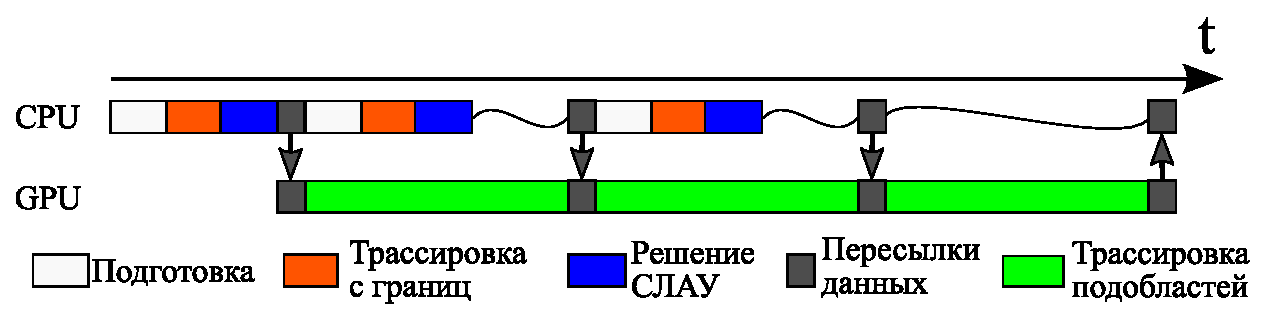
\includegraphics[width=0.8\linewidth]{timeline.eps}
\caption{Временная развертка алгоритма}
\label{fig:timeline}
\end{figure}
           % Глава 4
\chapter{Результаты}

Все численные методы были реализован в виде программ на языке C++ с использованием библиотеки CUDA \cite{cuda2015} для организации вычислений на графических процессорах. Использовались трехмерные сетки, сгенерированные программой NETGEN v4.9.14 \cite{Netgen2009}.
Для визуализации результатов применялась программа ParaView \cite{Paraview2004}.

\section{Исследование сходимости метода, основанного на вариационном принципе}

Исследование скорости сходимости проводились на задаче о плотности энергии излучения оптически плотного излучающего шара радиуса $R = 0.3$ в поглощающей оптически менее плотной среде (см. приложение \ref{sec:sphere}). В окрестности поверхности шара плотность энергии имеет логарифмическую особенность производной, такую же, как и в задаче Милна (задача об излучении из полупространства, см. приложение \ref{sec:milne}).

Изучалась ошибка в точках $A(0, 0, 0)$ --- центре шара, $B\left(\frac{R}{\sqrt{3}}, \frac{R}{\sqrt{3}}, \frac{R}{\sqrt{3}}\right)$ --- точке на границе шара в дискретной норме $L_2$:
\[
||u||_{DL_2} = \sqrt{\frac{1}{N}\sum_{i=1}^N u_i^2}
\]

Использовались пространственные сетки с количеством узлов от $7 \cdot 10^3$ до $206 \cdot 10^3$. Для метода сферических гармоник применялись сферические функции до $12$-й степени. Для метода радиальных базисных функций использовались $7$ первых квадратурных формул Лебедева в качестве сетки направлений. 

\subsection{Сходимость методов по количеству угловых функций}

Анализ сходимости в дискретной норме $L_2$ показал, что зависимость ошибки на самой подробной сетке ($206 \cdot 10^3$ узлов) от числа используемых угловых функций $K$ носит одинаковый характер $\varepsilon \sim K^{-0.29}$, причем ошибка обоих методов практически одинакова при одинаковом количестве используемых угловых функций, см. график на рисунке \ref{fig:UL2err}.

\begin{figure}[ht!]
\centering
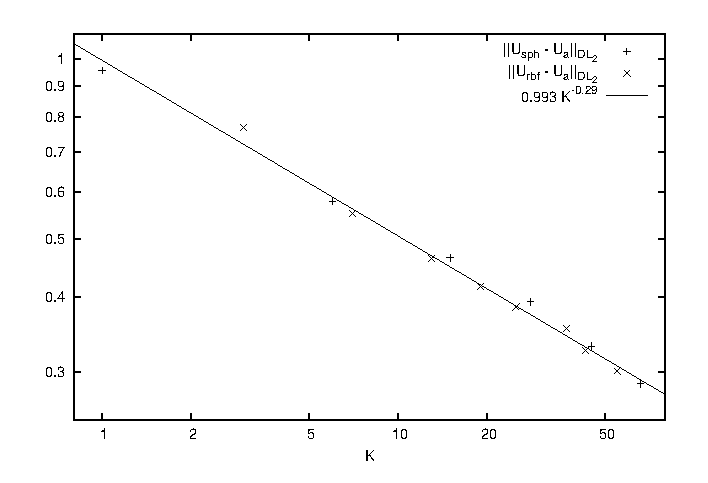
\includegraphics[width=\textwidth]{UL2err.eps}
\caption{Ошибка в норме $||\cdot||_{DL_2}$ в зависимости от числа угловых функций $K$}
\label{fig:UL2err}
\end{figure}

\subsection{Пространственная сходимость методов}

Сходимость методов изучалась в точке $A$ из области гладкости и в точке $B$ на границе шара при использовании самой подробной угловой дискретизации. Сходимость изучалась в зависимости от характерного шага пространственной сетки, принятого равным $N^{-1/3}$. На рисунке \ref{fig:UAerr} изображены графики ошибки в области гладкости и на границе шара.

\begin{figure}[ht!]
\centering
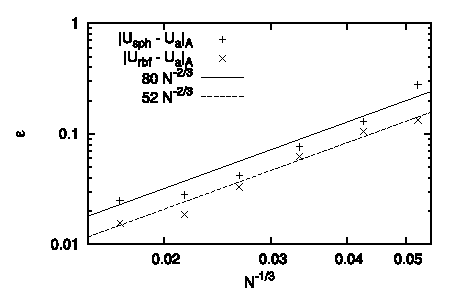
\includegraphics[width=.49\textwidth]{UAerr.eps}
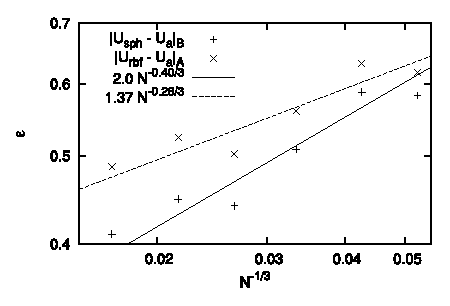
\includegraphics[width=.49\textwidth]{UBerr.eps}
\caption{Ошибка в точках $A, B$ в зависимости от характерного шага сетки $N^{-1/3}$}
\label{fig:UAerr}
\end{figure}

Порядок сходимости обоих методов в области гладкости равен двум. В области шара, где коэффициент поглощения меняется скачкообразно, порядок сходимости разный, он равен $\sim 0.4$ для метода сферических гармоник и $\sim 0.3$ для метода с радиальными базисными функциями, хотя разброс данных не позволяет достоверно определить порядок сходимости.

На рисунке \ref{fig:anvsnum} представлено решения вдоль оси $Ox$, полученные методом с радиальными функциями при $K = 55$ и методом сферических гармоник при $K = 91$. Видно, что существенное отличие численного решения от аналитического наблюдается в поглощающей области в окрестности шара.

Для обоих методов свойственны нефизичные значения интенсивности в области вдали от шара. Функция интенсивности, восстановленная из гармоник решения
\[
I(\vec r, \vec \Omega) = \sum_{k=1}^{n} I_k(\vec r) \theta_k (\vec \Omega)
\]
может содержать значения с отрицательными значениями интенсивности. В случае $I(\vec r, \vec \Omega) > 0$ тензор направленности излучения (тензор квазидиффузии) $\mathbb D$, определяемый как
\[
\mathbb D = \frac{\mathbb T}{U} = \frac{\int_{4\pi} \vec \Omega\vec \Omega I(\vec r, \vec \Omega) d\Omega}{\int_{4\pi} I(\vec r, \vec \Omega) d\Omega}
\]
имеет след, равный $1$ и неотрицательные компоненты. Однако, в численных расчетах свойство неотрицательности может нарушаться, если интенсивность $I(\vec r, \vec \Omega)$ принимает отрицательные значения (см. график на рисунке \ref{fig:Drad}). Значения $D_{rr} > 1$ свидетельствуют об отрицательности двух других главных компонент тензора $\mathbb D$.

\begin{figure}[ht!]
\centering
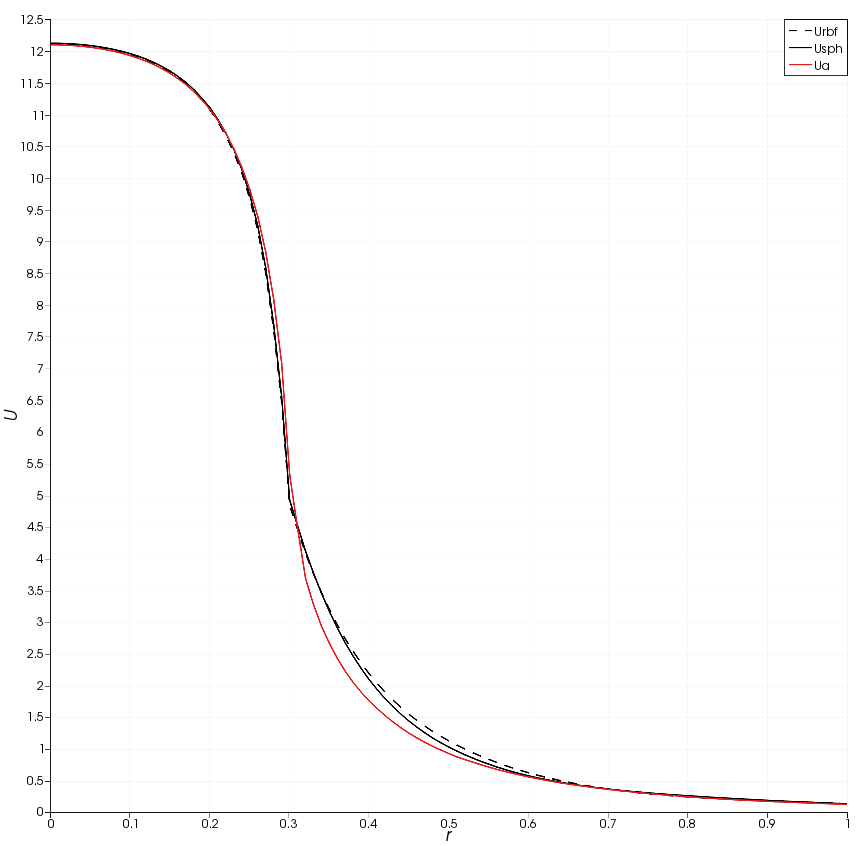
\includegraphics[width=.5\textwidth]{Uanvsnum.png}
\caption{Решения вдоль оси $Ox$, полученные методом с радиальными функциями при $K=55$ и методом сферических гармоник при $K = 91$}
\label{fig:anvsnum}
\end{figure}

\begin{figure}[ht!]
\centering
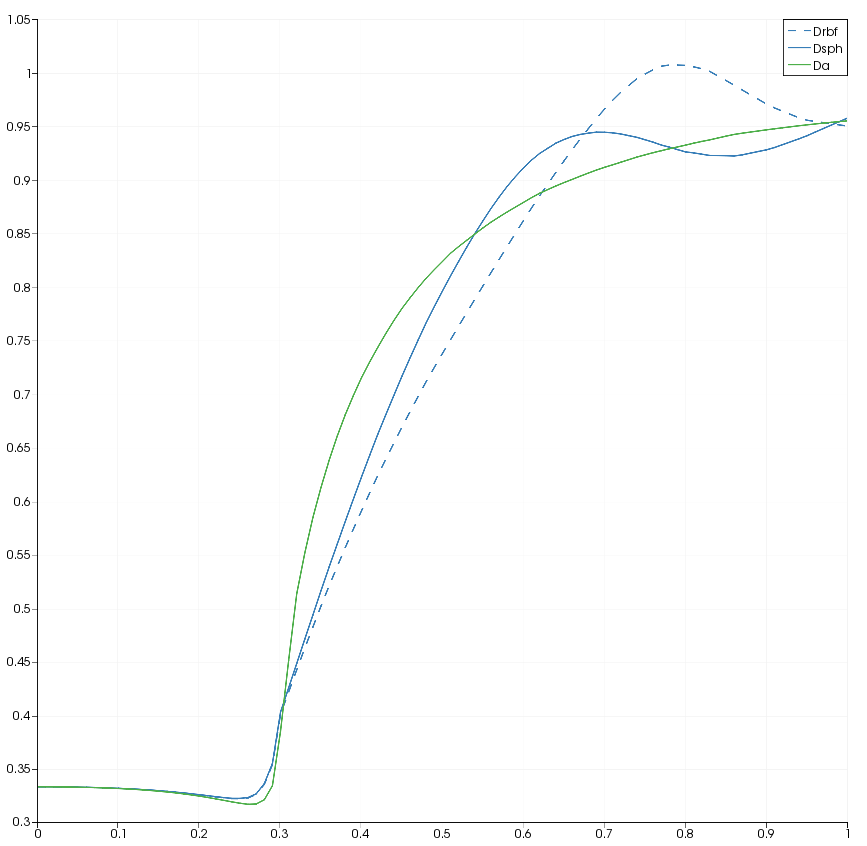
\includegraphics[width=.5\textwidth]{Dxx.png}
\caption{Радиальная компонента тензора направленноcти $\mathbb D_{rr}$ вдоль оси $Ox$}
\label{fig:Drad}
\end{figure}

Для исследования эффекта луча рассмотрим изоповерхности плотности интенсивности. Для метода сферических гармоник эффект луча отсутствует, поскольку базис из сферических функций инвариантен относительно произвольных вращений. На рисунке \ref{fig:iso} изображены изоповерхности решений, построенные для случая $K = 15$ метода сферических гармоник и $K = 13$ метода с радиальными функциями.

\begin{figure}[ht!]
\centering
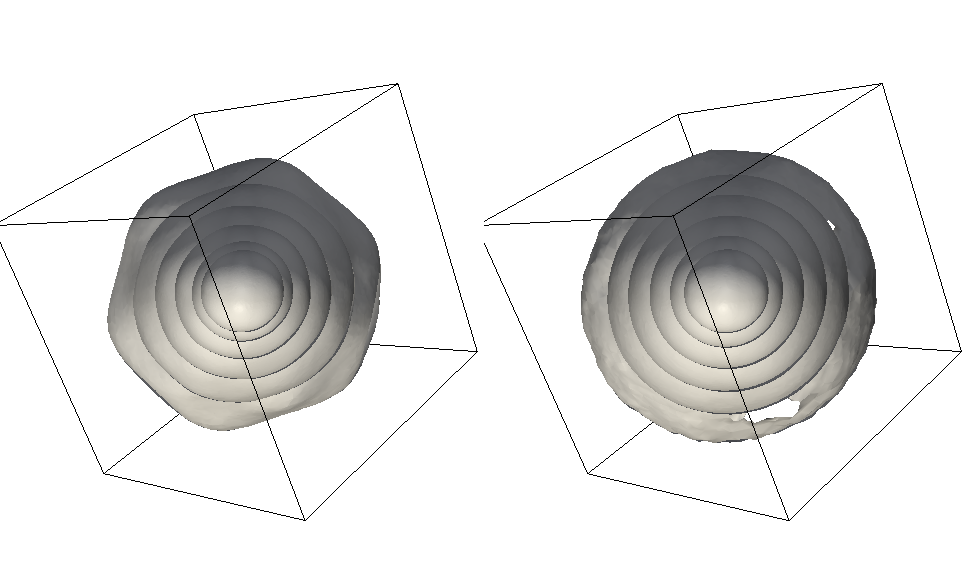
\includegraphics[width=\textwidth]{iso.png}
\caption{Изоповерхности плотности энергии излучения для метода с радиальными функциями (слева) и сферическими гармониками (справа)}
\label{fig:iso}
\end{figure}

\subsection{Сходимость метода при использовании предобуславливателя}

Для исследования сходимости внешних итераций метода сопряженных градиентов изучалось количество вызовов предобуславливателя, необходимых для уменьшения нормы невязки в $10^{6}$ раз.

Отметим, что для метода сопряженных градиентов число итераций увеличивается как с увеличением количества угловых гармоник $K$, так и увеличением количества узлов сетки $N$. Для метода с радиальным базисом число итераций практически постоянно и равно $30$.

\begin{table}[ht!]
\RawFloats
\centering
\caption{Количество итераций метода сопряженных градиентов}
\begin{tabular}{cc|c|c|c|c|c|c|}
\cline{3-8}
& & \multicolumn{6}{|c|}{\rule{0em}{2.2ex}Количество узлов сетки} \\ \cline{3-8}
& & \rule{0em}{2.2ex}6996 & 12971 & 26786 & 53109 & 99015 & 205756\\ \cline{1-8}
\multicolumn{1}{|c|}{\multirow{7}{*}{\rotatebox{90}{Угловых  гармоник\phantom{x}}}} &
\multicolumn{1}{|c|}{\rule{0em}{2.2ex}1}  & 1 & 1 & 1 & 1 & 1 & 1 \\ 
\cline{2-8}\multicolumn{1}{|c|}{} &
\multicolumn{1}{|c|}{\rule{0em}{2.2ex}6}  & 20 & 21 & 22 & 23 & 25 & 26 \\ 
\cline{2-8}\multicolumn{1}{|c|}{} &
\multicolumn{1}{|c|}{\rule{0em}{2.2ex}15} & 29 & 31 & 33 & 34 & 37 & 38 \\ 
\cline{2-8}\multicolumn{1}{|c|}{} &
\multicolumn{1}{|c|}{\rule{0em}{2.2ex}28} & 36 & 38 & 41 & 44 & 48 & 51 \\ 
\cline{2-8}\multicolumn{1}{|c|}{} &
\multicolumn{1}{|c|}{\rule{0em}{2.2ex}45} & 42 & 45 & 49 & 53 & 57 & 62 \\ 
\cline{2-8}\multicolumn{1}{|c|}{} &
\multicolumn{1}{|c|}{\rule{0em}{2.2ex}66} & 46 & 50 & 55 & 60 & 65 & 70 \\ 
\cline{2-8}\multicolumn{1}{|c|}{} &
\multicolumn{1}{|c|}{\rule{0em}{2.2ex}91} & 48 & 53 & 59 & 65 & 71 & 77 \\ 
\cline{1-8}
\end{tabular}
\end{table}

\begin{table}[ht!]
\RawFloats
\centering
\caption{Количество итераций метода с радиальным базисом}
\begin{tabular}{cc|c|c|c|c|c|c|}
\cline{3-8}
& & \multicolumn{6}{|c|}{\rule{0em}{2.2ex}Количество узлов сетки} \\ \cline{3-8}
& & \rule{0em}{2.2ex}6996 & 12971 & 26786 & 53109 & 99015 & 205756\\ \cline{1-8}
\multicolumn{1}{|c|}{\multirow{7}{*}{\rotatebox{90}{Угловых гармоник\phantom{x}}}} &
\multicolumn{1}{|c|}{\rule{0em}{2.2ex}3}  & 13 & 14 & 15 & 14 & 15 & 15 \\ 
\cline{2-8}\multicolumn{1}{|c|}{} &
\multicolumn{1}{|c|}{\rule{0em}{2.2ex}7}  & 26 & 27 & 28 & 28 & 29 & 31 \\ 
\cline{2-8}\multicolumn{1}{|c|}{} &
\multicolumn{1}{|c|}{\rule{0em}{2.2ex}13} & 33 & 34 & 35 & 36 & 39 & 42 \\ 
\cline{2-8}\multicolumn{1}{|c|}{} &
\multicolumn{1}{|c|}{\rule{0em}{2.2ex}19} & 26 & 28 & 29 & 29 & 30 & 32 \\ 
\cline{2-8}\multicolumn{1}{|c|}{} &
\multicolumn{1}{|c|}{\rule{0em}{2.2ex}25} & 28 & 29 & 32 & 30 & 32 & 34 \\ 
\cline{2-8}\multicolumn{1}{|c|}{} &
\multicolumn{1}{|c|}{\rule{0em}{2.2ex}43} & 28 & 30 & 32 & 31 & 33 & 34 \\ 
\cline{2-8}\multicolumn{1}{|c|}{} &
\multicolumn{1}{|c|}{\rule{0em}{2.2ex}55} & 27 & 28 & 30 & 29 & 30 & 32 \\ 
\cline{1-8}
\end{tabular}
\end{table}

\section{Исследование маршевого метода коротких характеристик}

Для метода коротких характеристик изучалась численная диффузия луча. Центральное излучательное тело было заменено на крест, составленный из пяти одинаковых кубов (см. рисунок \ref{fig:cross}). Уравнение переноса решалось в одном направлении, при этом аналитическое решение представляет собой проекцию креста на грань тетраэдра. Оптическая толщина излучающего тела много больше единицы, а оптическая толщина окружающего пространства много меньше единицы. В таких условиях, решение на грани имеет интенсивность равную равновесной интенсивности в кресте.
\begin{figure}[ht!]
\centering
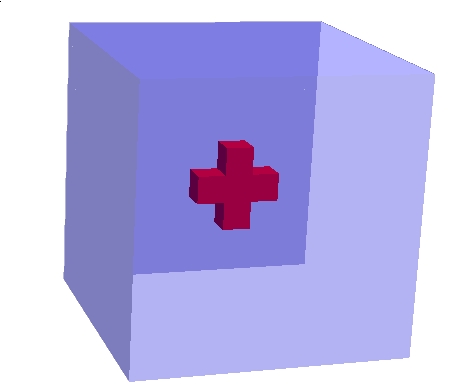
\includegraphics[width=.5\textwidth]{plus.png}
\caption{Вид излучающего тела для метода коротких характеристик}
\label{fig:cross}
\end{figure}

%\subsection{Сравнение численной диффузии луча в методах первого и второго порядка}

Для метода первого порядка решение на грани испытывает значительную диффузию. Для метода второго порядка без ограничителя решение нарушает принцип максимума. Отклонения интенсивности на грани от диапазона $[0, 1]$ составляет $20 \%$ (области на границе креста). Метод с ограничителем имеет решение, в котором принцип максимума не нарушен, а численная диффузия луча значительно меньше, чем в случае метода первого порядка.

\begin{figure}[ht!]
\centering
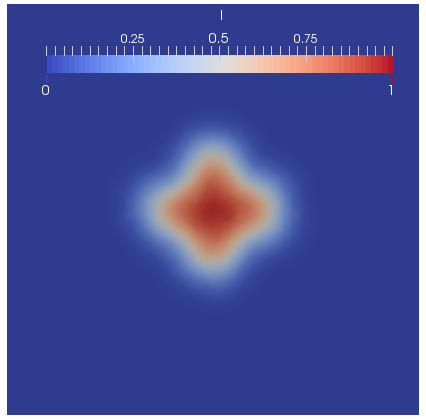
\includegraphics[width=.3\textwidth]{res1ord.png}
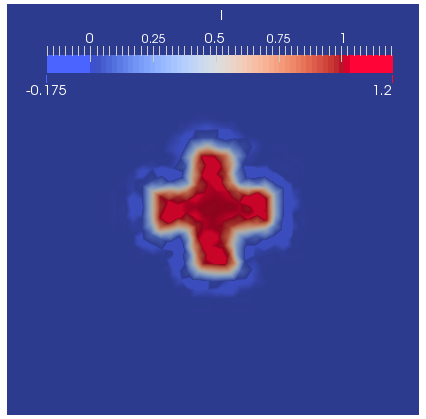
\includegraphics[width=.3\textwidth]{res2nolim.png}
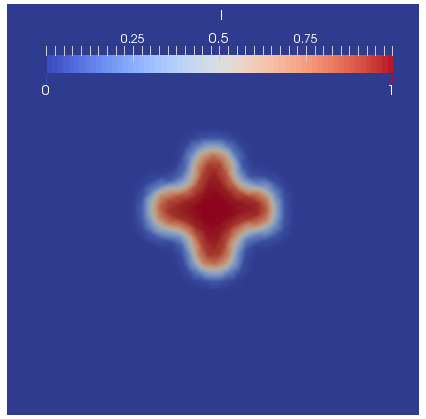
\includegraphics[width=.3\textwidth]{res2wilim.png}
\caption{Решение на грани для метода первого порядка (слева), метода второго порядка (в центре) и метода второго порядка с ограничителем (справа)}
\label{fig:limiter}
\end{figure}

Сравнение плотности излучения в решениях, полученных методом первого и второго порядка с ограничителем, показывает близкие (в пределах $2\%$) решения (см. графики на рисунках \ref{fig:U2vs1} и \ref{fig:U2vs1Line}). При этом для метода второго порядка плотность энергии излучения сосредоточена в кресте, в то время как в методе первого порядка она диффундирует за его пределы. К тому же, в методе второго порядка более выражен эффект луча, в методе же первого порядка он сглажен численной диффузией.

\begin{figure}[ht!]
\centering
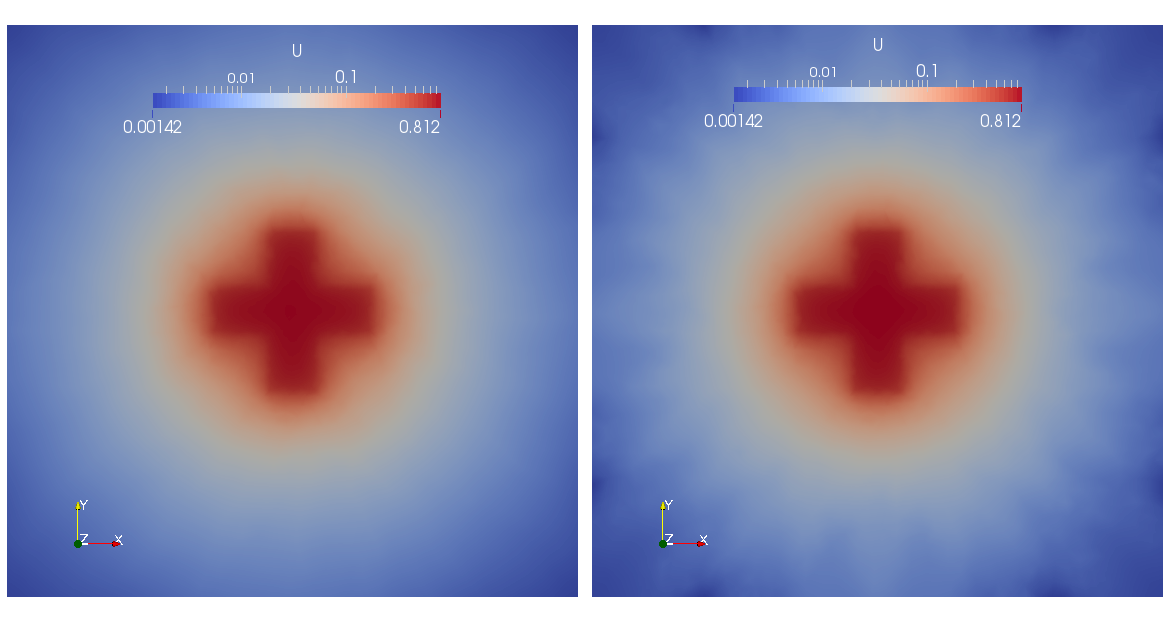
\includegraphics[height=.35\textheight]{U2vs1.png}
\caption{Плотность излучения в методе первого порядка (слева) и второго порядка с ограничителем (справа) в центральном сечении}
\label{fig:U2vs1}
\end{figure}

\begin{figure}[ht!]
\centering
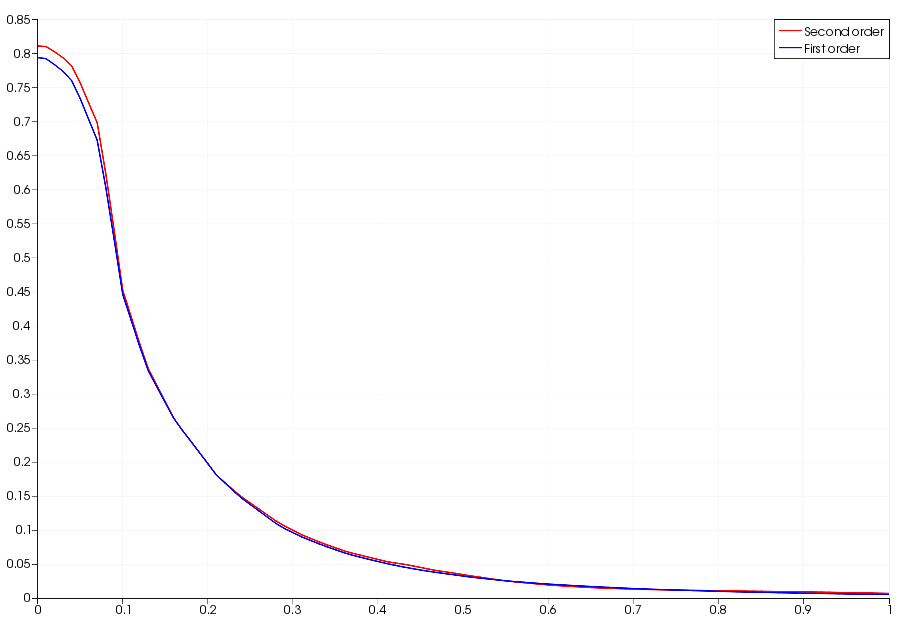
\includegraphics[height=.35\textheight]{U2vs1Line.png}
\caption{Плотность излучения в методе первого порядка (синий график) и второго порядка с ограничителем (красный график) вдоль луча, перпендикулярного кресту}
\label{fig:U2vs1Line}
\end{figure}

Дополнительно был рассмотрен метод первого порядка с увеличенным количеством узлов. В этом методе вместо квадратичной интерполяции по шести узлам используется кусочно-линейная. Данная операция позволяет сравнивать методы при одинаковом числе используемых узлов. 

Рассматривалась задача об излучении шара в сферической области. Поглощение в области отсутствовало. Диффузия луча носит качественно различный характер: в методе первого порядка диффузия луча имеет характер $\sim \sqrt{x}$, а в методе второго порядка диффузия луча постоянна вдоль луча, см. график на рисунке \ref{fig:diffus}.

\begin{figure}[ht!]
\centering
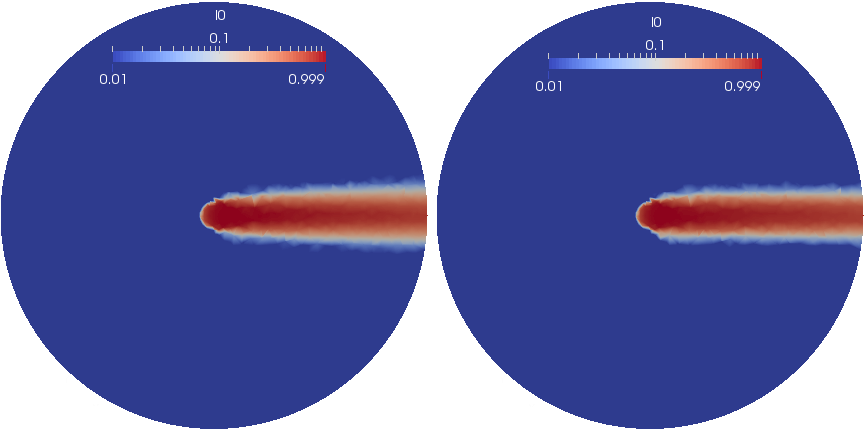
\includegraphics[width=\textwidth]{diff.png}
\caption{Диффузия луча в методе первого порядка с увеличенным числом узлов (слева) и методе второго порядка с ограничителем (справа)}
\label{fig:diffus}
\end{figure}

\section{Исследование распределенного метода длинных характеристик}

Данный метод тестировался на той же модельной задаче, что и метод, основанный на вариационном принципе. Использовалась пространственная сетка с $66 \cdot 10^{3}$ узлов ($363 \cdot 10^{3}$ тетраэдров) и угловая сетка из $230$ направлений (квадратурная формула Лебедева $25$-го порядка). Область разбивалась на $2, 3, 4$ и $8$ подобластей с помощью библиотеки METIS \cite{METIS}.  Для решения разреженной системы линейных уравнений применялась библиотека UMFPACK \cite{umfpack2004}. Для организации распределенных вычислений использовалась библиотека OpenMPI \cite{MPI}.

\subsection{Сравнение решений для различного числа подобластей}

В случае нескольких подобластей метод имеет незначительную диффузию луча, проходящего через поверхность раздела подобластей.
На рисунке \ref{fig:diff} приведены решения для случая одной подобласти и восьми подобластей. Численная диффузия в данном методе несоизмеримо меньше численной диффузии в методе коротких характеристик.
На рисунке \ref{fig:split} можно видеть разбиение области на подобласти (показаны 4 из 8).

\begin{figure}[ht!]
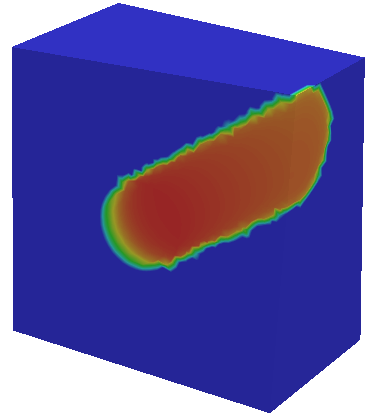
\includegraphics[width=.35\textwidth]{res1piece}
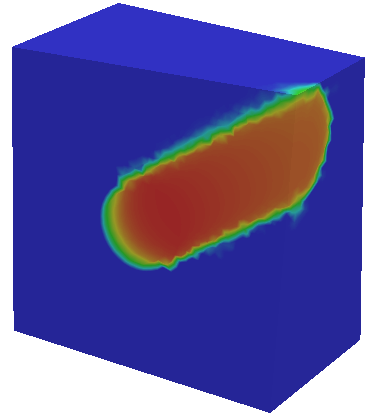
\includegraphics[width=.35\textwidth]{res8pieces}
\caption{Срез решения в одном направлении. Слева одна подобласть, справа --- 8}
\label{fig:diff}
\end{figure}

\begin{figure}[ht!]
\centering
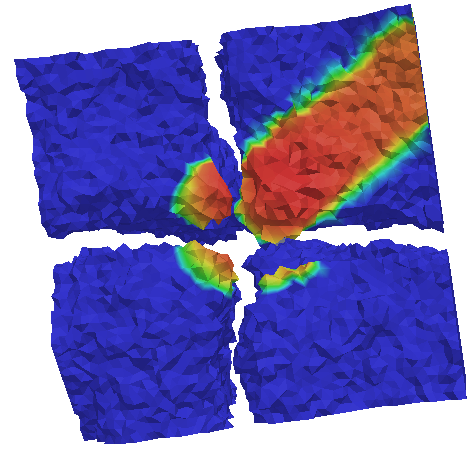
\includegraphics[width=.35\textwidth]{ressplit.png}
\caption{Используемая декомпозиция области на подобласти}
\label{fig:split}
\end{figure}

Если пренебречь численной диффузией, метод имеет эталонную точность для каждого направления. Однако, это приводит к наиболее выраженному эффекту луча среди всех исследованных методов, см. изоповерхности решения на рисунке \ref{fig:isomcm}. Наиболее выражены искажения вдоль координатных осей $Ox, Oy, Oz$. В этих направлениях веса квадратурной формулы Лебедева максимальны.

\begin{figure}[ht!]
\centering
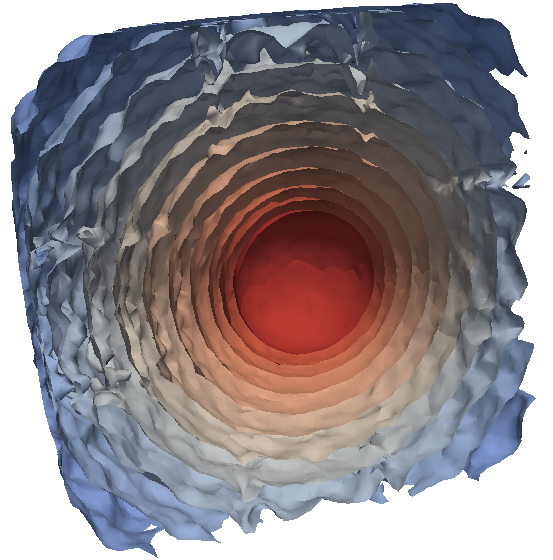
\includegraphics[width=.4\textwidth]{isomcm.png}
\caption{Изоповерхности плотности излучения, полученной распределенным методом длинных характеристик}
\label{fig:isomcm}
\end{figure}

\subsection{Ускорение и эффективность параллельной реализации}

В таблице \ref{tab:speedup} приведено сравнение времени работы алгоритма при различных разбиениях расчетной области. Данные результаты получены на высокопроизводительном стенде кафедры информатики и вычислительной математики МФТИ. Незначительное ускорение обусловлено хаотическим доступом к памяти при трассировке лучей, плохой балансировкой нагрузки на графическом ускорителе, а также значительным количеством условных операторов в коде трассировки. 
\begin{table}[ht!]
\RawFloats
\centering
\caption{Время работы алгоритма в зависимости от числа подобластей $P$ для MPI-реализации (CPU) и MPI+CUDA-реализации (GPU)}
\begin{tabular}{|c|c|c|c|c|}
\hline
$P$ & Устройства & $t_\text{GPU}, \text{c}$ & $t_\text{CPU}, \text{c}$ & $t_\text{CPU} / t_\text{GPU}$\\\hline
$1$& 1 $\times$ Tesla C2075 & $117$ & $439$ & $3.75$x\\\hline
$2$& 2 $\times$ Tesla C2075 & $52$ & $196$ & $3.77$x\\\hline
$3$& 3 $\times$ Tesla C2075 & $32.7$ & $125$ & $3.82$x\\\hline
$4$& 3 $\times$ Tesla C2075 + GTX 680 & $28.1$ & $108$ & $3.84$x\\
%    $4$& 1 x Tesla C2075 & $88$ & $108$ & $1,23$x\\
\hline
$8$& 3 $\times$ Tesla C2075 + GTX 680 & $25.5$ & $69$ & $2.70$x\\\hline
\end{tabular}
\label{tab:speedup}
\end{table}

Отметим сверхлинейное ускорение как CPU, так и GPU версии программы. Оно вызвано тем, что распределенный метод не является параллельной версией метода длинных характеристик, а является другим параллельным методом, решение которого зависит от числа подобластей и способа разбиения. Если не принимать во внимание это обстоятельство, эффективность распараллеливания
\[
E_P = \frac{S_P}{P}, \quad S = \frac{t_1}{t_P}
\]
достигает $120 \%$ при $P = 3$. Сверхлинейное ускорение вызвано уменьшением средней длины характеристики при разбиении области на подобласти. Учитывая, что при разбиении на $3$ подобласти средняя длина характеристики сокращается в $\sqrt[3]{3} \approx 1.44$ раз, реальная эффективность распараллеливания составляет 
\[
\tilde E_P = \frac{E_P}{\sqrt[3]{P}}.
\]
Для $P=2$ эта величина равна $\tilde E = \frac{117}{2 \cdot 52 \sqrt[3]{2}} \approx 89 \%$, а для $P = 3$ --- $\tilde E_3 = \frac{117 \%}{3 \cdot 32.7\sqrt[3]{3}} \approx 83 \%$. Аналогичные показатели для реализации с графическими ускорителями отличаются незначительно.

\section{Расчет спектра излучения линии H-$\alpha$ звезды типа Т Тельца}

Для численного воспроизведения спектра излучения линии H-$\alpha$ были использованы поля гидродинамических величин из работы \cite{romanova2009}. В этой работе с помощью математического моделирования изучалось взаимодействие звезды с ее аккреционным диском. Магнитный момент звезды составлял угол в $30^\circ$ к направлению вращения звезды, что при определенных условиях падения вещества на звезду приводило к образованию конического ветра (см. рисунок \ref{fig:wind}).
\begin{figure}[ht!]
\centering
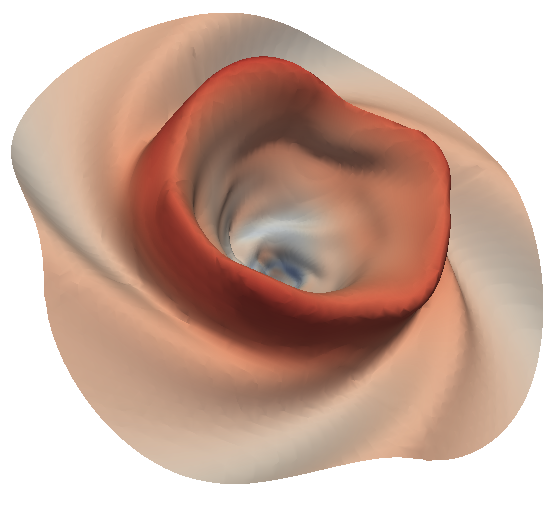
\includegraphics[width=.4\textwidth]{wind.png}
\caption{Изоповерхность плотности вещества, окружающего звезду. Цвет соответствует величине радиальной компоненты скорости}
\label{fig:wind}
\end{figure}

В работе \cite{romanova2009} расчет проводится в безразмерных единицах, а результаты могут быть применены к широкому набору астрофизических задач подстановкой конкретных размерных единиц, при условии сохранения тех же безразмерных определяющих параметров. Значения размерных единиц были подставлены для случая классической звезды Т Тельца. Также, был проведен расчет с увеличенным значением единицы измерения магнитного поля $B_0 = 40 \text{ Гс}$ вместо $B_0 = 12.5 \text{ Гс}$, что соответствует увеличению единицы измерения плотности в $10$ раз, без изменения характерного масштаба длины. 

В работе \cite{romanova2009} приняты следующие размерные единицы: 
\begin{itemize}
\item единица измерения длины $R_0 = 2 R_*$, где $R_*$ --- радиус звезды;
\item единица измерения массы $M_0 = M_*$, где $M_*$ --- масса звезды;
\item единица измерения скорости $v_0 = \sqrt\frac{GM}{R_0}$ --- единица скорости;
\item единица измерения магнитного поля $B_0 = \frac{B_*}{\bar \mu} \left(\frac{R_*}{R_0}\right)^3$, где $B_*$ --- магнитное поле на поверхности звезды, $\bar \mu$ --- безразмерный магнитный момент звезды;
\item единица измерения температуры $T_0 = \frac{v_0^2}{\mathcal R}$, где $\mathcal R$ --- универсальная газовая постоянная;
\item единица измерения плотности $\rho_0 = \frac{B_0^2}{v_0^2}$
\item единица измерения давления $p_0 = B_0^2 = \frac{\rho_0}{\mathcal{R} T_0}$.
\end{itemize}

Подставляя безразмерные единицы в формулы для коэффициента поглощения \eqref{eq:absorb}, получаем 
\[
R_0 \varkappa_\nu(v_0 \Delta \tilde v) = \frac{\varkappa \lambda_0 R_0}{v_0} \frac{1}{\sqrt{2\pi \tilde T}} \exp\left(
-\frac{(\Delta  \tilde v + \tilde {\vec v} \vec k)^2}{2\tilde T}
\right),
\]
где величины с тильдой являются обезразмеренными.

В качестве расчетной области использовалась полусфера, увеличенная так, чтобы содержать центральное излучающее тело --- звезду. Расчетная сетка состояла из $713 \cdot 10^3$ узлов ($4 \cdot 10^6$ тетраэдров). Расчет проводился распределенным методом длинных характеристик.
Использовалась равномерная по полярному углу сетка направлений. Для каждого значения полярного угла
азимутальная сетка строилась так, чтобы расстояние между соседними направлениями было приблизительно одинаковым. Угловая сетка содержала $1091$ направление. Такая сетка позволила получить усредненные по периоду обращения звезды спектры при различных углах наклонения $i$ (угол между плоскостью диска и лучом зрения). Использовалось $64$ частотные группы в интервале, соответствующем доплеровскому смещению линии H-$\alpha$ от $-600 \text{ км}/\text{c}$ до $600 \text{ км}/\text{c}$. Для каждого направления $\vec \omega_i$ вычислялся интегральный поток излучения, уходящего с поверхности шара в направлении $\vec \omega_i$. Также, благодаря использованию распределенного метода длинных характеристик, стало возможным отключить блок трассировки внутренности подобластей, что значительно сократило время вычислений. Для расчетов использовались два узла кластера лаборатории флюидодинамики и сейсмоакустики МФТИ, на каждом узле использовалось 8 графических ускорителей. На данной задаче было достигнуто ускорение $4.5$ раза по отношению к MPI-реализации без использования графических ускорителей.

Зависимость усредненной за период обращения звезды относительной интенсивности $I_\text{o}$ от частоты излучения при разных углах наклонения $i$ представлена на рисунке \ref{fig:spectre}. Для удобства смещение частоты $\Delta \nu$ переведено в относительную скорость $\Delta v = c \frac{\Delta \nu}{\nu_0}$. Можно заключить, что при углах наклонения $i \lesssim 45^\circ$ поглощение в диапазоне синего смещения $\Delta v \sim 150 \dividesymbol 200 \text{ км}/\text{с}$ существенно лишь для случая $B_0 = 40 \text{ Гс}$. Нормализованный профиль линии излучения имеет существенный провал в области красного смещения на скорости $\Delta v \approx 100 \text{ км}/\text{с}$, который объясняется значительным поглощением излучения веществом диска, аккрецирующего на звезду. Для случая $B_0 = 12.5 \text{ Гс}$ существенное поглощение в линии спектра наблюдается лишь для направлений, близких к плоскости диска. 
\begin{figure}[ht!]
\centering
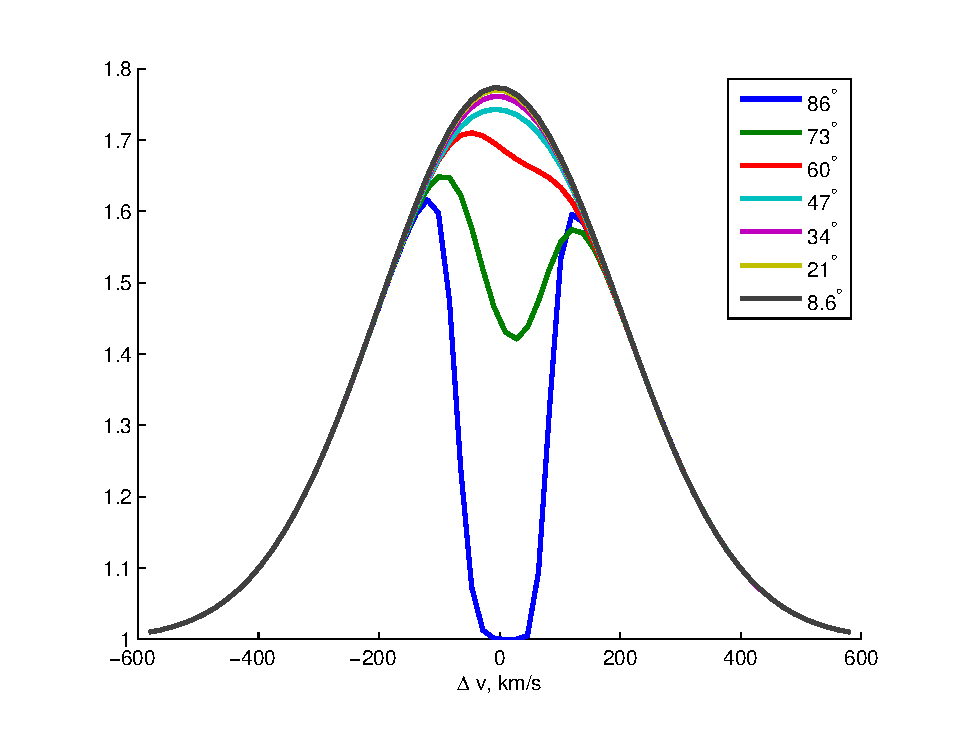
\includegraphics[width=.6\textwidth]{spectrum-bad.eps}
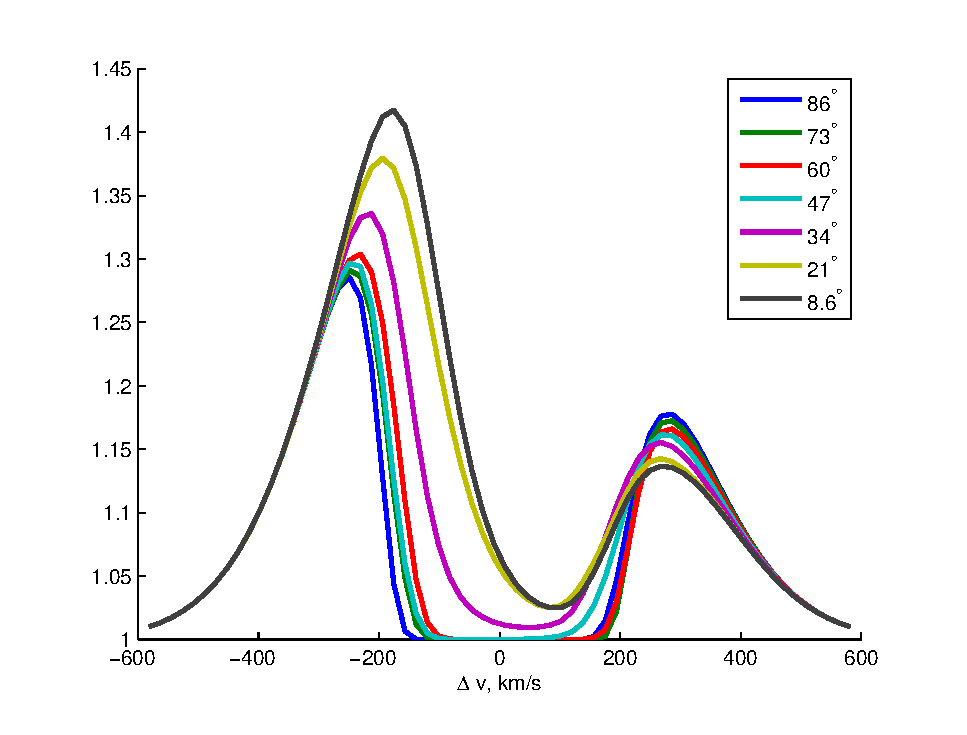
\includegraphics[width=.6\textwidth]{spectrum.eps}
\caption{Профиль линии H-$\alpha$ в зависимости от угла наклонения $i$ для случая $B_0 = 12.5 \text{ Гс}$ (сверху) и $B_0 = 40 \text{ Гс}$ (снизу)}
\label{fig:spectre}
\end{figure}

\FloatBarrier

\section{Выводы}

Основанные на вариационном принципе методы (метод сферических гармоник и метод с радиальным базисом)  демонстрируют сходное поведение: оба метода сходятся со вторым порядком в области гладкости и с порядком, меньшим единицы, в области особенности градиента решения. Ошибка в дискретной норме $L_2$ не зависит от типа угловой дискретизации, а зависит лишь от количества угловых функций $K$. Метод с радиальными базисными функциями сходится за меньшее количество вызовов предобуславливателя, но не обладает свойством инвариантности относительно поворотов, то есть имеет выделенные направления.

Для метода коротких характеристик второго порядка осцилляции могут составлять до $20\%$. Использование ограничителя полностью их устраняет. В методе второго порядка сильнее выражен эффект луча, в то время, как в методе первого порядка, он сглажен из-за численной диффузии. Точность метода второго порядка обусловлена не только повышенным числом узлов, так как метод второго порядка оказался более точным по сравнению с методом, использующим кусочно-линейную интерполяцию по шести точкам.

Распределенный метод длинных характеристик обладает высокой точностью метода длинных характеристик. Решения, полученные данным методом, имеют незначительную диффузию луча, проходящего через границу раздела подобластей. Эффект луча в данном методе выражен наиболее сильно. Реализация метода с использованием графических ускорителей показала ускорение примерно в $4$ раза относительно MPI-версии. Такое незначительное ускорение может быть объяснено случайным доступом к памяти и плохой балансировкой загрузки нитей.

Проведено численное моделирование формы линии H-$\alpha$ в спектре звезды Т Тельца из работы \cite{romanova2009}. Показано, что  поглощение наблюдается не только в области синего смещения, но и в области красного смещения. Поглощение в области красного смещения вызвано веществом, аккрецирующем на звезду.
           % Глава 5
\chapter*{Заключение}						% Заголовок
\addcontentsline{toc}{chapter}{Заключение}	% Добавляем его в оглавление

%% Согласно ГОСТ Р 7.0.11-2011:
%% 5.3.3 В заключении диссертации излагают итоги выполненного исследования, рекомендации, перспективы дальнейшей разработки темы.
%% 9.2.3 В заключении автореферата диссертации излагают итоги данного исследования, рекомендации и перспективы дальнейшей разработки темы.
%% Поэтому имеет смысл сделать эту часть общей и загрузить из одного файла в автореферат и в диссертацию:

Основные результаты работы:
%% Согласно ГОСТ Р 7.0.11-2011:
%% 5.3.3 В заключении диссертации излагают итоги выполненного исследования, рекомендации, перспективы дальнейшей разработки темы.
%% 9.2.3 В заключении автореферата диссертации излагают итоги данного исследования, рекомендации и перспективы дальнейшей разработки темы.
\begin{enumerate}
  \item Для решения уравнения переноса излучения разработан вариационный метод с радиальными базисными функциями, который обладает точностью, сравнимой с точностью метода сферических гармоник, но при этом является более экономичным. Экономичность была достигнута за счет использования
  предложенного блочно-диагонального предобуславливания метода решения системы линейных уравнений. 
  Построены оптимальные квадратурные формулы для полусферы, инвариантные относительно группы вращений.
  \item Разработан маршевый метод коротких характеристик. Построены варианты данного метода первого и второго порядка аппроксимации. Получено условие расположения узлов, выполнение которого необходимо для устойчивости метода второго порядка. Для монотонизации схемы второго порядка применен ограничитель значения интенсивности в дополнительных узлах.
  \item Для маршевого метода построены алгоритмы упорядочения неструктурированных сеток. Дополнительным результатом работы алгоритмов упорядочения является ярусно-параллельная форма графа зависимостей вычислительного метода, которую можно использовать для распараллеливания процесса решения задачи. 
  \item Разработана версия метода длинных характеристик, адаптированная для распределенной реализации на многопроцессорных системах и на кластерах с графическими ускорителями. Исследованы ускорение и эффективность реализаций метода в зависимости от числа используемых вычислительных узлов и графических ускорителей.
  \item Разработанные вычислительные алгоритмы реализованы в виде программного комплекса. В рамках модели локального термодинамического равновесия вычислен коэффициент поглощения частично ионизованной плазмы. Для задачи моделирования спектра излучения звезды типа Т Тельца построен спектральный профиль линии H-$\alpha$ в зависимости от ориентации плоскости аккреционного диска.
\end{enumerate}


Дальнейшее развитие методов, основанных на вариационном принципе, возможно в направлении ускорения работы за счет использования быстрых численных методов решения эллиптических задач типа квазидиффузии. Вариационная постановка Владимирова может быть развита для учета более сложных граничных условий и коэффициента поглощения, зависящего от направления. Использование распределенных алгоритмов решения уравнения квазидиффузии позволит реализовать этот метод для многопроцессорных вычислительных систем.

Сохранение неотрицательности решения и выполнение принципа максимума являются трудными задачами в методе, основанном на вариационном принципе, и, по-видимому, требуют введения нелинейности в целевой минимизируемый функционал.

Перспективным видится объединение метода коротких характеристик и распределенного метода длинных характеристик. С помощью метода коротких характеристик возможно достаточно быстро построить разностный оператор Грина, хотя он уже не может быть представлен компактно из-за численной диффузии луча. Однако, можно выделить небольшое число (например, 20) узлов, где содержится существенная часть носителя оператора Грина. При этом основной принцип составления линейной системы, включающей только граничные неизвестные, остается таким же, как и в распределенном методе длинных характеристик.
      % Заключение
\clearpage                                  % В том числе гарантирует, что список литературы в оглавлении будет с правильным номером страницы
\phantomsection
\addcontentsline{toc}{chapter}{\bibname}	% Добавляем список литературы в оглавление
%\hypersetup{ urlcolor=black }               % Ссылки делаем чёрными
%\providecommand*{\BibDash}{}                % В стилях ugost2008 отключаем использование тире как разделителя 
\urlstyle{rm}                               % ссылки URL обычным шрифтом
\insertbibliofull                          % Подключаем Bib-базы
\urlstyle{tt}                               % возвращаем установки шрифта ссылок URL
%\hypersetup{ urlcolor={urlcolor} }          % Восстанавливаем цвет ссылок
      % Список литературы
\appendix
%% Правка оформления ссылок на приложения:
%http://tex.stackexchange.com/questions/56839/chaptername-is-used-even-for-appendix-chapters-in-toc
%http://tex.stackexchange.com/questions/59349/table-of-contents-with-chapter-and-appendix
%% требует двойной компиляции
\addtocontents{toc}{\def\protect\cftchappresnum{\appendixname{} }%
\setlength{\cftchapnumwidth}{\widthof{\cftchapfont\appendixname~Ш\cftchapaftersnum}}%
}
%% Оформление заголовков приложений ближе к ГОСТ:
\sectionformat{\chapter}[display]{% Параметры заголовков разделов в тексте
    label=\chaptertitlename\ \thechapter,% (ГОСТ Р 2.105, 4.3.6)
    labelsep=20pt,
}
\renewcommand\thechapter{\Asbuk{chapter}} % Чтобы приложения русскими буквами нумеровались
\chapter{Задачи с аналитическим решением}
\newcommand{\Ip}{I_\text{p}}
\label{chap:problem}

\section{Задача об излучающем шаре}
\label{sec:sphere}

В бесконечной среде с коэффициентом поглощения $\varkappa = \varkappa_1$ с равновесным излучением $\Ip = 0$ находится 
шар из материала с $\varkappa = \varkappa_2$, однородно излучающий с $\Ip = I_0$.
\begin{figure}[ht!]%
\centering%
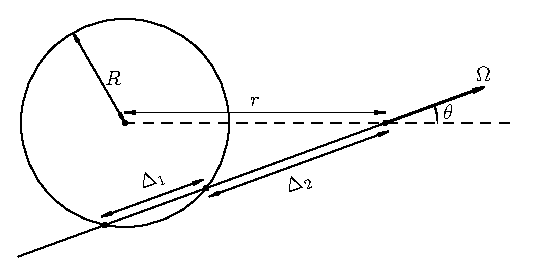
\includegraphics[width=0.5\columnwidth]{box-0}%
\quad%
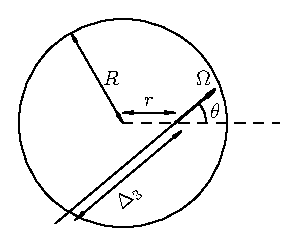
\includegraphics[width=0.27\columnwidth]{box-1}%
\caption{К построению решения уравнения переноса вдоль луча}%
\end{figure}

Переменные, изображенные на рисунке равны:
\begin{gather*}
\Delta_1 = 2\sqrt{R^2 - r^2 \sin^2 \theta}\\
\Delta_2 = r \cos \theta - \sqrt{R^2 - r^2 \sin^2 \theta}\\
\Delta_3 = r \cos \theta + \sqrt{R^2 - r^2 \sin^2 \theta}.
\end{gather*}

Уравнение переноса вдоль луча можно записать в виде
\begin{align*}
\frac{dI(s)}{ds} + \varkappa I = \varkappa \Ip.
\end{align*}

В точке $-\infty$ интенсивность равна нулю, она продолжает не изменяться, пока луч не дойдет до шара. Как только луч окажется в шаре, интенсивность
будет нарастать по закону \mbox{$I_0(1-e^{-\varkappa_2 \Delta s})$}. На выходе из шара интенсивность будет равна 
\mbox{$I_0(1-e^{-\varkappa_2 \Delta_1})$}. Далее, интенсивность снова спадает 
по экспоненциальному закону.
\begin{align*}
I(r,\theta) = I_0
\begin{cases}
1-e^{-\varkappa_2 \left(r \cos \theta + \sqrt{R^2 - r^2 \sin^2 \theta}\right)},&R > r\\
\left(1-e^{-2\varkappa_2\sqrt{R^2 - r^2 \sin^2 \theta}}\right)
e^{-\varkappa_1 \left(r \cos \theta - \sqrt{R^2 - r^2 \sin^2 \theta}\right)},&\theta < \arcsin \frac{R}{r}\\
0,&\text{иначе}
\end{cases}.
\end{align*}
Найдем плотность энергии излучения, поток энергии вдоль радиуса и компоненту $rr$ тензора потока импульса
\begin{align*}
U(r) &= \frac{1}{c} \int\limits I(r,\Omega) d\Omega = \frac{2\pi}{c} \int\limits_0^\pi I(r, \theta) \sin \theta d\theta\\
S_r(r) &= \int\limits \Omega_r I(r,\Omega) d\Omega = 2\pi \int\limits_0^\pi \cos \theta I(r, \theta) \sin \theta d\theta\\
T_{rr}(r) &= \frac{1}{c} \int\limits \Omega_r^2 I(r,\Omega) d\Omega = \frac{2\pi}{c} \int\limits_0^\pi \cos^2 \theta I(r, \theta) \sin \theta d\theta.
\end{align*}
Заменим $\cos \theta = \mu, \sin^2 \theta = 1-\mu^2$. Интегрирование заменится по правилу
\begin{align*}
\int\limits_0^\pi \bullet \sin \theta d\theta = \int\limits_{-1}^1 \bullet d\mu.
\end{align*}
Интенсивность в новых обозначениях примет вид
\begin{align*}
I(r,\mu) = I_0
\begin{cases}
1-e^{-\varkappa_2 \left(\mu r + \sqrt{R^2 - (1-\mu^2)r^2}\right)},&R > r\\
\left(1-e^{-2\varkappa_2\sqrt{R^2 - (1-\mu^2)r^2}}\right)
e^{-\varkappa_1 \left(\mu r- \sqrt{R^2 - (1-\mu^2)r^2}\right)},&\mu > \sqrt{1-\frac{R^2}{r^2}}\\
0,&\text{иначе}
\end{cases},
\end{align*}
а $U, S_r$ и $T_{rr}$ соответственно
\begin{align*}
U(r) &= \frac{2\pi}{c} \int\limits_{-1}^{1} I(r, \mu) d\mu\\
S_r(r) &= 2\pi \int\limits_{-1}^1 \mu I(r, \mu) d\mu\\
T_{rr}(r) &= \frac{2\pi}{c} \int\limits_{-1}^1 \mu^2 I(r, \mu) d\mu
\end{align*}
Также можно рассмотреть тензор направленности излучения $\mathbb D = \frac{1}{U} \mathbb{T}$. В случае изотропного излучения $\hat D = \frac{1}{3}\mathbb I$

\begin{figure}[ht!]%
\centering
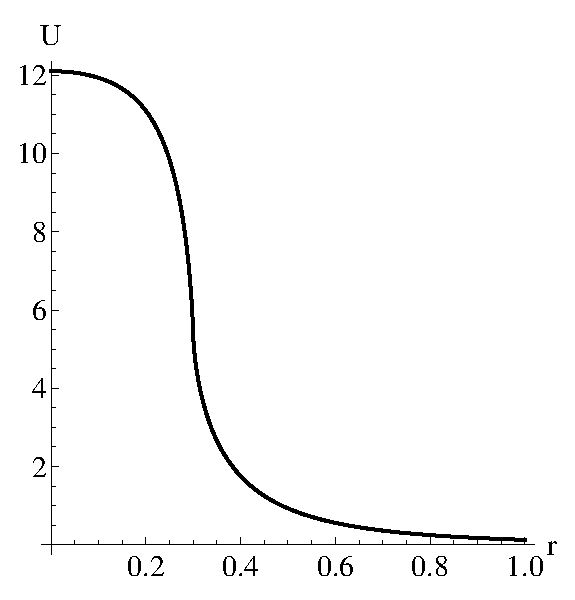
\includegraphics[width=.3\columnwidth]{U}\quad%
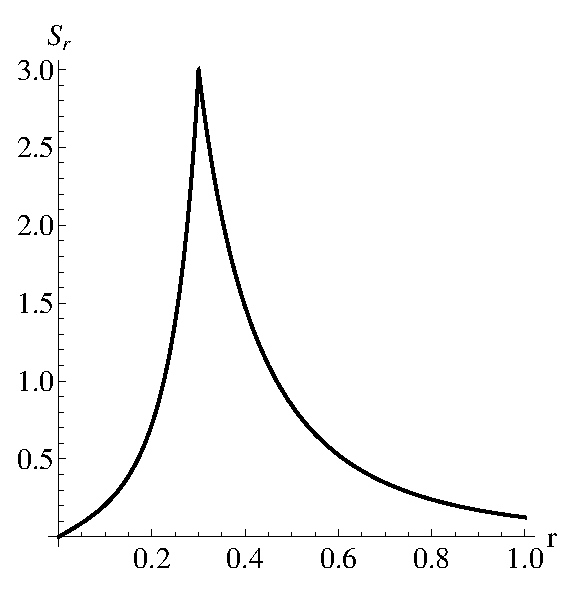
\includegraphics[width=.3\columnwidth]{S.eps}\quad%
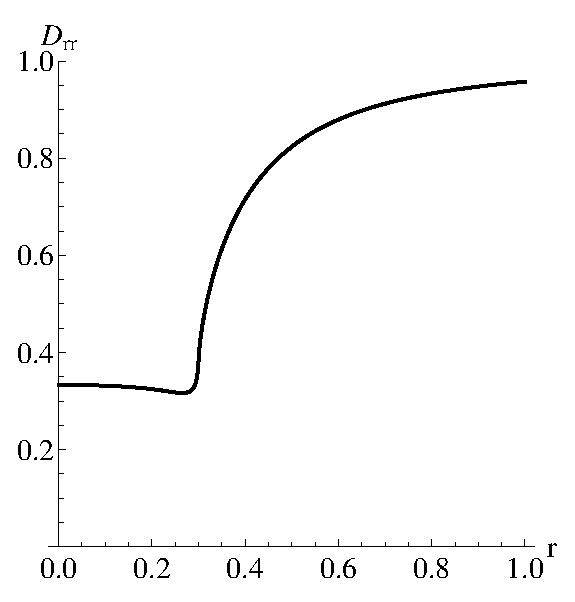
\includegraphics[width=.3\columnwidth]{Drr}%
\caption{Графики плотности энергии, потока энергии и направленности излучения при $R = 0.3, I_0 = 1, c = 1, \varkappa_1 = 1, \varkappa_2 = 11$}%
\end{figure}

\section{Задача о двух полупространствах (задача Милна)}
\label{sec:milne}

Пространство при $x < 0$ заполнено веществом с коэффициентом поглощения $\varkappa_1$ и интенсивностью равновесного излучения $\Ip = I_1$,
а при $x \geq 0$ --- веществом с коэффициентом поглощения $\varkappa_2$ и интенсивностью равновесного излучения $\Ip = I_2$.

\begin{figure}[ht!]%
\centering

\includegraphics[height=2in]{half-0}%
\caption{К определению интенсивности из уравнения вдоль луча}%
\label{pic:halfspace}%
\end{figure}
Для определенности будем искать $I$ при $x > 0$. 
Величина $\Delta$ на рисунке равна $\frac{x}{\cos \theta}$. Запишем уравнение переноса вдоль луча
\begin{equation*}
\frac{dI(s)}{ds} + \varkappa I = \varkappa \Ip.
\end{equation*}
Обозначим $\mu = \cos \theta$. При $\mu > 0$ интенсивность в $-\infty$ равна равновесной интенсивности в левой области $I_1$.
После пересечения плоскости $x = 0$ решение по экспоненциальному закону $I_1 + (I_2 - I_1) (1 - e^{-\varkappa_2 s})$
стремится к равновесному излучению в правой области. При $\mu \leq 0$, интенсивность равна равновесной интенсивности в правой области $I_2$:
\begin{equation*}
I(x, \mu) = \begin{cases}
I_2 + (I_1 - I_2) e^{-\varkappa_2 \Delta}, &\,\mu > 0\\
I_2 , &\,\mu \leq 0
\end{cases}
\end{equation*}
Аналогично предыдущей задаче,
\begin{align}
U &= \frac{2\pi}{c} \int\limits_{-1}^1 I(x, \mu) d\mu\\
S_x &= 2\pi \int\limits_{-1}^1 \mu I(x, \mu) d\mu\\
T_{xx} &= \frac{2\pi}{c} \int\limits_{-1}^1 \mu^2 I(x, \mu) d\mu
\end{align}
Интегрируя, получаем
\begin{align}
U &= \frac{4\pi}{c} I_2 + \frac{2\pi}{c}(I_1 - I_2)\int\limits_0^1 e^{-\frac{z}{\mu}} d\mu = \nonumber\\
&=\frac{4\pi}{c} I_2 + \frac{2\pi}{c}(I_1 - I_2)\left(e^{-z} + z 
\operatorname{Ei}(-z)\right)\\
S_x &= 2\pi (I_1 - I_2)\int\limits_{0}^1 \mu e^{-\frac{z}{\mu}} d\mu = \nonumber\\
&= \pi (I_1 - I_2) \left((1 - z)e^{-z} - z^2
\operatorname{Ei}(-z)\right)\\
T_{xx} &= \frac{4\pi}{3c}I_2 + \frac{2\pi}{c} (I_1 - I_2)\int\limits_{0}^1 \mu^2 e^{-\frac{z}{\mu}} d\mu = 
\nonumber\\
&= \frac{4\pi}{3c}I_2 + \frac{\pi}{3c} (I_1 - I_2)\left((2 - z + z^2)e^{-z} + z^3 \operatorname{Ei}(-z)\right),
\end{align}
где $z = \varkappa_2 x$ --- оптическое расстояние от границы до точки $x$. Решения при $x < 0$ поулчаются
заменой первой среды на вторую и $z$ на $-z$.
\begin{figure}[ht!]%
\centering
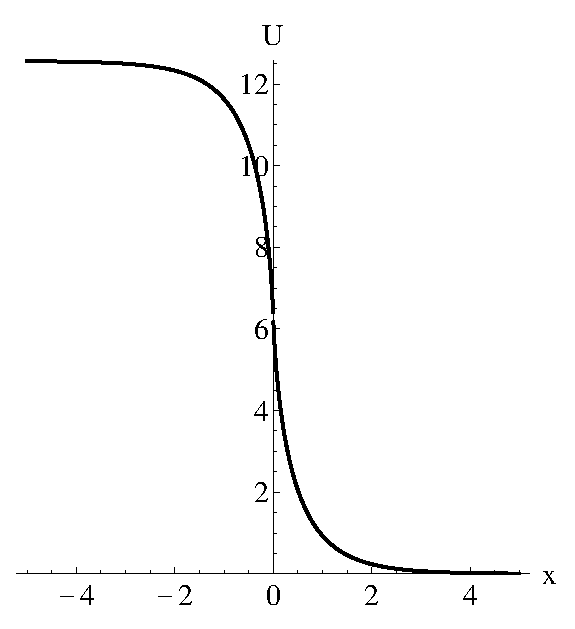
\includegraphics[width=.3\columnwidth]{U2}\quad%
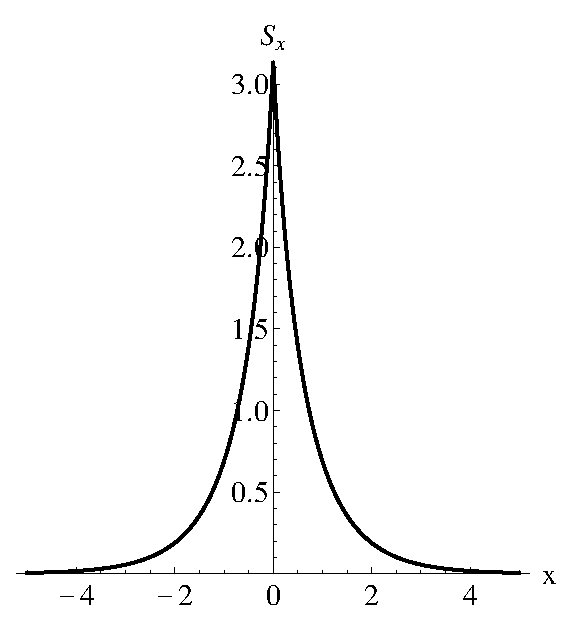
\includegraphics[width=.3\columnwidth]{S2}\quad%
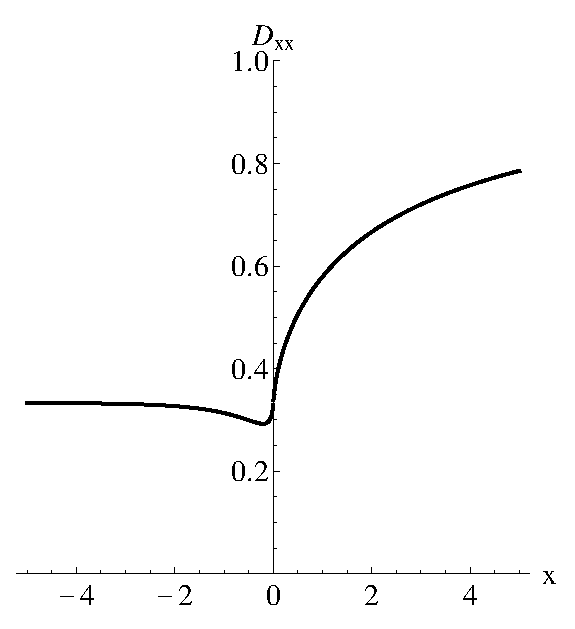
\includegraphics[width=.3\columnwidth]{D2xx}%
\caption{Графики плотности энергии, потока энергии и направленности излучения при $I_2 = 0, I_1 = 1, c = 1$
в зависимости от оптического расстояния от границы}%
\end{figure}
       % Приложения 
\chapter{Сферические функции}
\label{chap:spher}

\section{Сферические функции, используемые в работе}

В работе были использованы действительные сферические функции, образующие ортонормированную систему по отношению
к скалярному произведению $(\varphi, \psi) = \frac{1}{4\pi} \int \varphi \psi d\Omega$. Они имеют следующее представление
\begin{align*}
Y_{l,m}(\theta, \varphi) &= C_{l,m}P_l^{m}(\cos \theta)\times
\begin{cases}
\sin |m| \varphi,&\, m<0\\
\frac{1}{\sqrt{2}},&\, m=0\\
\cos m \varphi,&\, m>0\\
\end{cases}
\label{eq:sphfunc}\\
C_{l,m} &= (-1)^{\frac{|m|+m}{2}}\sqrt{4l+2}\sqrt{\frac{(l-m)!}{(l+m)!}},
\end{align*}
где $P^m_l(\mu)$ --- присоединенный многочлен Лежандра степени $l$ и порядка $m$.

Сферические функции могут быть выражены как однородные многочлены от компонент $\vec \Omega$. Представление нескольких первых 
функций приведено ниже:
\begin{align*}
Y_{0,0} &= 1\\
Y_{1,-1} = \sqrt{3}\Omega_y,\quad
Y_{1,0} &= \sqrt{3}\Omega_z,\quad
Y_{1,1} = \sqrt{3}\Omega_x\\
Y_{2,-2} = \sqrt{15}\Omega_x\Omega_y,\quad
Y_{2,-1} &= \sqrt{15}\Omega_y\Omega_z, \quad
Y_{2,1} = \sqrt{15}\Omega_x\Omega_z\\
Y_{2,0} = \sqrt{5}\Omega_z^{2}&-\frac{\sqrt{5}}{2}\Omega_y^{2}-\frac{\sqrt{5}}{2}\Omega_x^{2}\\
Y_{2,2} = \frac{\sqrt{15}}{2}\Omega_x^{2}&-\frac{\sqrt{15}}{2}\Omega_y^{2}
\end{align*}

\section{Правила отбора для интеграла от трех действительных сферических функций}
\label{sec:select}

Рассмотрим следующий интеграл
\[
\begin{bmatrix}
l_1 & l_2 & l_3\\
m_1 & m_2 & m_3
\end{bmatrix} \equiv
\int\limits_{4\pi}
Y_{l_1,m_1}(\vec \Omega)
Y_{l_2,m_2}(\vec \Omega)
Y_{l_3,m_3}(\vec \Omega)
d\Omega.
\]
Без ограничений общности, предположим, что $l_1 \leq l_2 \leq l_3$.
Найдем необходимые условия, при которых он отличен от нуля. Учтем, что сферические функции допускают представление
\[
Y_{l,m}(\vec \Omega) = C_{l,m} P_l^{m}(\cos \theta) \Phi_m(\varphi),
\]
а, следовательно, рассматриваемый интеграл может быть записан как
\begin{multline*}
\begin{bmatrix}
l_1 & l_2 & l_3\\
m_1 & m_2 & m_3
\end{bmatrix} =
C_{l_1,m_1}
C_{l_2,m_2}
C_{l_3,m_3} \times \\ \times
\int\limits_{-1}^1 
P_{l_1}^{m_1}(\mu)
P_{l_2}^{m_2}(\mu)
P_{l_3}^{m_3}(\mu)
d\mu
\int\limits_{0}^{2\pi}
\Phi_{m_1}(\varphi)
\Phi_{m_2}(\varphi)
\Phi_{m_3}(\varphi)
d\varphi
\end{multline*}
Для интеграла
\[
\int\limits_{-1}^1 
P_{l_1}^{m_1}(\mu)
P_{l_2}^{m_2}(\mu)
P_{l_3}^{m_3}(\mu)
d\mu
\]
известны \cite{Gaunt1929} правила отбора, которые заключаются в том, что интеграл не равен нулю только если выполнены следующие предположения:
\begin{itemize}
\item сумма степеней $l_1 + l_2 + l_3$ четна;
\item степени удовлетворяют неравенству треугольника $l_3 < l_1 + l_2$.
\end{itemize}

Для интеграла 
\[
\int\limits_{0}^{2\pi}
\Phi_{m_1}(\varphi)
\Phi_{m_2}(\varphi)
\Phi_{m_3}(\varphi)
d\varphi
\]
рассмотрим возможные случаи.
\paragraph{Случай $m_1 = 0$.} Поскольку $\Phi_0(\varphi) = \frac{1}{\sqrt{2}}$, интеграл сводится к 
\[
\int\limits_{0}^{2\pi}
\Phi_{m_2}(\varphi)
\Phi_{m_3}(\varphi)
d\varphi,
\]
который отличен от нуля только при $m_2 = m_3$.
\paragraph{Случай $m_1 \leq m_2 \leq m_3 < 0$.} Интеграл представим в виде
\begin{multline*}
-\int\limits_{0}^{2\pi}
\sin m_1 \varphi
\sin m_2 \varphi
\sin m_3 \varphi
d\varphi = \\ 
= 
\frac{1}{2}\int\limits_{0}^{2\pi}
\sin m_1 \varphi
\cos (m_2 + m_3) \varphi
d\varphi 
-
\frac{1}{2}\int\limits_{0}^{2\pi}
\sin m_1 \varphi
\cos (m_3 - m_2) \varphi
d\varphi.
\end{multline*}
Оба интеграла равны нулю. 

\paragraph{Случай $m_1 \leq m_2 < 0 < m_3$.} Интеграл представим в виде
\begin{multline*}
\int\limits_{0}^{2\pi}
\sin m_1 \varphi
\sin m_2 \varphi
\cos m_3 \varphi
d\varphi = \\ 
= 
\frac{1}{2}\int\limits_{0}^{2\pi}
\cos (m_2 - m_1) \varphi
\cos m_3 \varphi
d\varphi 
+
\frac{1}{2}\int\limits_{0}^{2\pi}
\cos (m_1 + m_2) \varphi
\cos m_3 \varphi
d\varphi.
\end{multline*}
Интеграл отличен от нуля если $m_3 = m_2 - m_1$ либо $m_3 = -m_1 - m_2$.

\paragraph{Случай $m_1 < 0 < m_2 \leq m_3$.} Интеграл представим в виде
\begin{multline*}
-\int\limits_{0}^{2\pi}
\sin m_1 \varphi
\cos m_2 \varphi
\cos m_3 \varphi
d\varphi = \\ 
= 
-\frac{1}{2}\int\limits_{0}^{2\pi}
\sin m_1 \varphi
\cos (m_2 + m_3) \varphi
d\varphi 
-
\frac{1}{2}\int\limits_{0}^{2\pi}
\sin m_1 \varphi
\cos (m_2 - m_3) \varphi
d\varphi.
\end{multline*}
Оба интеграла равны нулю. 

\paragraph{Случай $0 < m_1 \leq m_2 \leq m_3$.} Интеграл представим в виде
\begin{multline*}
\int\limits_{0}^{2\pi}
\cos m_1 \varphi
\cos m_2 \varphi
\cos m_3 \varphi
d\varphi = \\ 
= 
\frac{1}{2}\int\limits_{0}^{2\pi}
\cos m_1 \varphi
\cos (m_2 + m_3) \varphi
d\varphi 
+
\frac{1}{2}\int\limits_{0}^{2\pi}
\cos m_1 \varphi
\cos (m_2 - m_3) \varphi
d\varphi.
\end{multline*}
Интеграл отличен от нуля только если $m_1 + m_2 = m_3$ (случай $m_1 = m_2 + m_3$ невозможен, т.к. $m_3 \geq m_1, m_2 > 0$).

Подытожим, интеграл 
\[
\int\limits_{0}^{2\pi} \Phi_{m_1}(\varphi)\Phi_{m_2}(\varphi)\Phi_{m_3}(\varphi) d\varphi, \quad 
m_1 \leq m_2 \leq m_3,
\]
отличен от нуля только если
\begin{itemize}
\item одно из чисел $m_1, m_2, m_3$ равно нулю, а остальные равны между собой;
\item либо $m_1, m_2, m_3 > 0$ и $m_3 = m_1 + m_2$;
\item либо $m_1, m_2 < 0, m_3 > 0$, при этом либо $m_1 + m_2 + m_3 = 0$, либо $m_1 - m_2 + m_3 = 0$.
\end{itemize}
В совокупности с правилами отбора для степеней $l_1, l_2, l_3$
\begin{itemize}
\item сумма степеней $l_1 + l_2 + l_3$ четна;
\item степени удовлетворяют неравенству треугольника $l_3 < l_1 + l_2$,
\end{itemize}
эти требования составляют правила отбора для интеграла
\[
\begin{bmatrix}
l_1 & l_2 & l_3\\
m_1 & m_2 & m_3
\end{bmatrix} \equiv
\int\limits_{4\pi}
Y_{l_1,m_1}(\vec \Omega)
Y_{l_2,m_2}(\vec \Omega)
Y_{l_3,m_3}(\vec \Omega)
d\Omega.
\]

\section{Матрица \texorpdfstring{$\mathscr{K}^{\alpha\beta}_{kk'}$}{K\^ab\_kk'} приближения \texorpdfstring{$K = 6$}{K = 6} метода сферических гармоник}
\label{sec:oioj}

Для иллюстрации разреженной структуры матрицы, приведен вариант при $n = 2$. Блоки соответствуют следующей нумерации сферических гармоник: 
$\varphi_{0,0}\quad \varphi_{2,-2}\quad \varphi_{2,-1}\quad \varphi_{2,0}\quad \varphi_{2,1}\quad \varphi_{2,2}$

\begin{small}
\begin{align*}
%&\langle \Omega_i \Omega_j \rangle_{2k\,m}^{2k'\,m'} = \\
%&
\left(
\begin{array}{@{}c@{}c@{}c||c@{}cc|cc@{}c|c@{}c@{}c|ccc|@{}c@{}c@{}c@{}}
\frac{1}{3}&0&0&
0&\frac{\sqrt{15}}{15}&0&
0&0&0&
-\frac{\sqrt{5}}{15}&0&0&
0&0&\frac{\sqrt{15}}{15}&
\frac{\sqrt{15}}{15}&0&0\\
0&\frac{1}{3}&0&
\frac{\sqrt{15}}{15}&0&0&
0&0&\frac{\sqrt{15}}{15}&
0&-\frac{\sqrt{5}}{15}&0&
0&0&0&
0&-\frac{\sqrt{15}}{15}&0\\
0&0&\frac{1}{3}&
0&0&0&
0&\frac{\sqrt{15}}{15}&0&
0&0&\frac{2\sqrt{5}}{15}&
\frac{\sqrt{15}}{15}&0&0&
0&0&0\\
\hline
\hline
0&\frac{\sqrt{15}}{15}&0&
\frac{3}{7}&0&0&
0&0&\frac{1}{7}&
0&-\frac{2\sqrt{3}}{21}&0&
0&0&0&
0&0&0\\
\frac{\sqrt{15}}{15}&0&0&
0&\frac{3}{7}&0&
0&0&0&
-\frac{2\sqrt{3}}{21}&0&0&
0&0&\frac{1}{7}&
0&0&0\\
0&0&0&
0&0&\frac{1}{7}&
\frac{1}{7}&0&0&
0&0&0&
0&\frac{1}{7}&0&
0&0&0\\
\hline
0&0&0&
0&0&\frac{1}{7}&
\frac{1}{7}&0&0&
0&0&0&
0&\frac{1}{7}&0&
0&0&0\\
0&0&\frac{\sqrt{15}}{15}&
0&0&0&
0&\frac{3}{7}&0&
0&0&\frac{\sqrt{3}}{21}&
\frac{1}{7}&0&0&
0&0&-\frac{1}{7}\\
0&\frac{\sqrt{15}}{15}&0&
\frac{1}{7}&0&0&
0&0&\frac{3}{7}&
0&\frac{\sqrt{3}}{21}&0&
0&0&0&
0&-\frac{1}{7}&0\\
\hline
-\frac{\sqrt{5}}{15}&0&0&
0&-\frac{2\sqrt{3}}{21}&0&
0&0&0&
\frac{5}{21}&0&0&
0&0&\frac{\sqrt{3}}{21}&
-\frac{2\sqrt{3}}{21}&0&0\\
0&-\frac{\sqrt{5}}{15}&0&
-\frac{2\sqrt{3}}{21}&0&0&
0&0&\frac{\sqrt{3}}{21}&
0&\frac{5}{21}&0&
0&0&0&
0&\frac{2\sqrt{3}}{21}&0\\
0&0&\frac{2\sqrt{5}}{15}&
0&0&0&
0&\frac{\sqrt{3}}{21}&0&
0&0&\frac{11}{21}&
\frac{\sqrt{3}}{21}&0&0&
0&0&0\\
\hline
0&0&\frac{\sqrt{15}}{15}&
0&0&0&
0&\frac{1}{7}&0&
0&0&\frac{\sqrt{3}}{21}&
\frac{3}{7}&0&0&
0&0&\frac{1}{7}\\
0&0&0&
0&0&\frac{1}{7}&
\frac{1}{7}&0&0&
0&0&0&
0&\frac{1}{7}&0&
0&0&0\\
\frac{\sqrt{15}}{15}&0&0&
0&\frac{1}{7}&0&
0&0&0&
\frac{\sqrt{3}}{21}&0&0&
0&0&\frac{3}{7}&
\frac{1}{7}&0&0\\
\hline
\frac{\sqrt{15}}{15}&0&0&
0&0&0&
0&0&0&
-\frac{2\sqrt{3}}{21}&0&0&
0&0&\frac{1}{7}&
\frac{3}{7}&0&0\\
0&-\frac{\sqrt{15}}{15}&0&
0&0&0&
0&0&-\frac{1}{7}&
0&\frac{2\sqrt{3}}{21}&0&
0&0&0&
0&\frac{3}{7}&0\\
0&0&0&
0&0&0&
0&-\frac{1}{7}&0&
0&0&0&
\frac{1}{7}&0&0&
0&0&\frac{1}{7}
\end{array}
\right)
\end{align*}
\end{small}       % Приложения 

\end{document}
